\documentclass[aps,prd,twocolumn,superscriptaddress,nofootinbib,longbibliography,floatfix,amsmath,amssymb,10pt]{revtex4-2}
\usepackage[utf8]{inputenc}
\usepackage[T1]{fontenc}
\usepackage{mathptmx}
\usepackage{amsthm}
\usepackage{mathrsfs}
\usepackage{graphicx}
\usepackage{booktabs}
\usepackage{multirow}
\usepackage{xcolor}
\usepackage{enumitem}
\usepackage[colorlinks=true,linkcolor=blue!50!black,citecolor=blue!50!black,urlcolor=blue!50!black]{hyperref}
\usepackage{orcidlink}
\usepackage[protrusion=true,expansion=false]{microtype}
\usepackage{xurl}
\makeatletter\let\write@bibliographystyle\relax\let\bibliography@latex\@gobble\makeatother

\theoremstyle{plain}
\newtheorem{theorem}{Theorem}[section]
\newtheorem{proposition}[theorem]{Proposition}
\newtheorem{lemma}[theorem]{Lemma}
\newtheorem{corollary}[theorem]{Corollary}
\theoremstyle{definition}
\newtheorem{definition}[theorem]{Definition}
\newtheorem{example}[theorem]{Example}
\newtheorem{remark}[theorem]{Remark}
\theoremstyle{plain}
\newtheorem{mainthm}{Theorem}
\renewcommand{\themainthm}{\Alph{mainthm}}

\newcommand{\NN}{\mathbb{N}}
\newcommand{\RR}{\mathbb{R}}
\newcommand{\EE}{\mathbb{E}}
\newcommand{\PR}{\mathbb{P}}
\newcommand{\eps}{\varepsilon}
\newcommand{\ind}{\mathbf{1}}
\newcommand{\Vs}{V^{*}}
\newcommand{\lean}[1]{\texttt{#1}}
\newcommand{\rr}{\raggedright\let\\\tabularnewline}
\tolerance=2000
\emergencystretch=2em
\hbadness=2000
\hfuzz=1pt

\begin{document}

\title{Beyond the LLM: BLLM and the Entropy Law of Sound Recursive Self-Improvement}

\author{Deep Bhattacharjee\,\orcidlink{0000-0003-0466-750X}}
\email{itsdeep@live.com}
\thanks{$*$\,Corresponding author. Second address: \nolinkurl{d.bhattacharjee@erl-forschung.de}.}
\affiliation{Formerly, Electro-Gravitational Space Propulsion Laboratory (EGSPL), Bhubaneswar, Odisha 751030, India}
\affiliation{Formerly, University of Calcutta, Senate House, 87/1 College Street, Kolkata 700073, West Bengal, India}

\author{Ushashi Bhattacharya\,\orcidlink{0009-0002-2254-3914}}
\email{rai.bhattacharya.in@gmail.com}
\affiliation{Formerly, National Taiwan University, Taipei 106319, Taiwan}

\date{October 18, 2026}

\begin{abstract}
\itshape
A BLLM is a language model that keeps a modification of itself only after a randomized check of soundness $\eps$ accepts it. We prove that the least cost of certifying modifications of total cost $A$ with at most $\theta$ expected false acceptances is $\frac{A}{\log(1/\eps)}\bigl(H(p)+\log\frac1\theta\bigr)$ up to an additive $A$, where $H(p)$ is the entropy of the cost profile, and that an infinite self-improvement of finite cost can be made sound exactly when $\sum_{n}a_{n}\log(1/a_{n})$ converges. The same price is paid online, without knowledge of future costs, up to a doubly logarithmic term that no online rule avoids, and it splits exactly over subagents.
\par\medskip\upshape\noindent\textit{2020 Mathematics Subject Classification.} 68T01; 68T05; 94A17; 60J80.\par\smallskip\noindent\textit{Keywords.} Recursive self-improvement; verification; entropy; branching processes.
\end{abstract}

\keywords{recursive self-improvement; verification; entropy; branching processes}

\maketitle
\makeatletter\renewcommand\l@subsection[2]{}\renewcommand\l@subsubsection[2]{}\makeatother
\tableofcontents

\section{Introduction}\label{sec:intro}

A system that rewrites its own weights, its own code or its own proofs, and keeps a rewrite when a test passes, is the basic unit of every proposal for recursive self-improvement. Good described the end point in 1965: a machine that designs a better machine, which designs a better one still, in an ``intelligence explosion'' that leaves human intelligence far behind \cite{Goo66}.\footnote{I.~J. Good, \emph{Speculations concerning the first ultraintelligent machine}, written in 1965 and printed in Advances in Computers, volume~6 (1966), pages 31--88 \cite{Goo66}. Good's argument is that an ultraintelligent machine could design better machines, so the first such machine is ``the last invention that man need ever make, provided that the machine is docile enough to tell us how to keep it under control''. The proviso is the subject of the present paper in a precise form: the docility we ask for is that every improvement the machine keeps has been checked, and we compute what the checking costs.} The literature since then has asked mostly how fast such a process could grow, under which assumptions on the returns to intelligence it reaches a vertical asymptote, and which physical limits stop it \cite{Ord26,AOA25,BSS26}. This paper asks a different question with a sharper answer: what does it cost to make sure that what the process keeps is correct?

We call the object a \emph{BLLM}, a system beyond the language model. It has three parts (Fig.~\ref{fig:architecture}). A generator, which may be a large language model \cite{VSP17,BMR20}, proposes candidate modifications of the system. A bank of randomized checks tests each candidate; a check has perfect completeness, so a correct candidate always passes, and soundness $\eps<1$, so an incorrect candidate passes one run with probability at most $\eps$. A memory keeps a candidate only after it has passed every run allotted to it, and the generator works from the memory. The word is taken from the verifier-gated engine of \cite{Bha26a}, whose escalation from token-level to beyond-token reasoning is the informal model here; the checks are the learned verifiers of \cite{CKB21,UKK22,LKB23}, the randomized identity tests of \cite{Sch80,Zip79}, the interactive and probabilistically checkable proofs of \cite{GMR89,Bab85,AS98,ALM98}, or a proof checker such as Lean \cite{MU21} run on a randomized search. The cost of a run of the check of the $i$-th candidate is $a_{i}>0$, and the schedule gives that check $r_{i}$ independent runs.

\begin{figure*}[t]
\centering
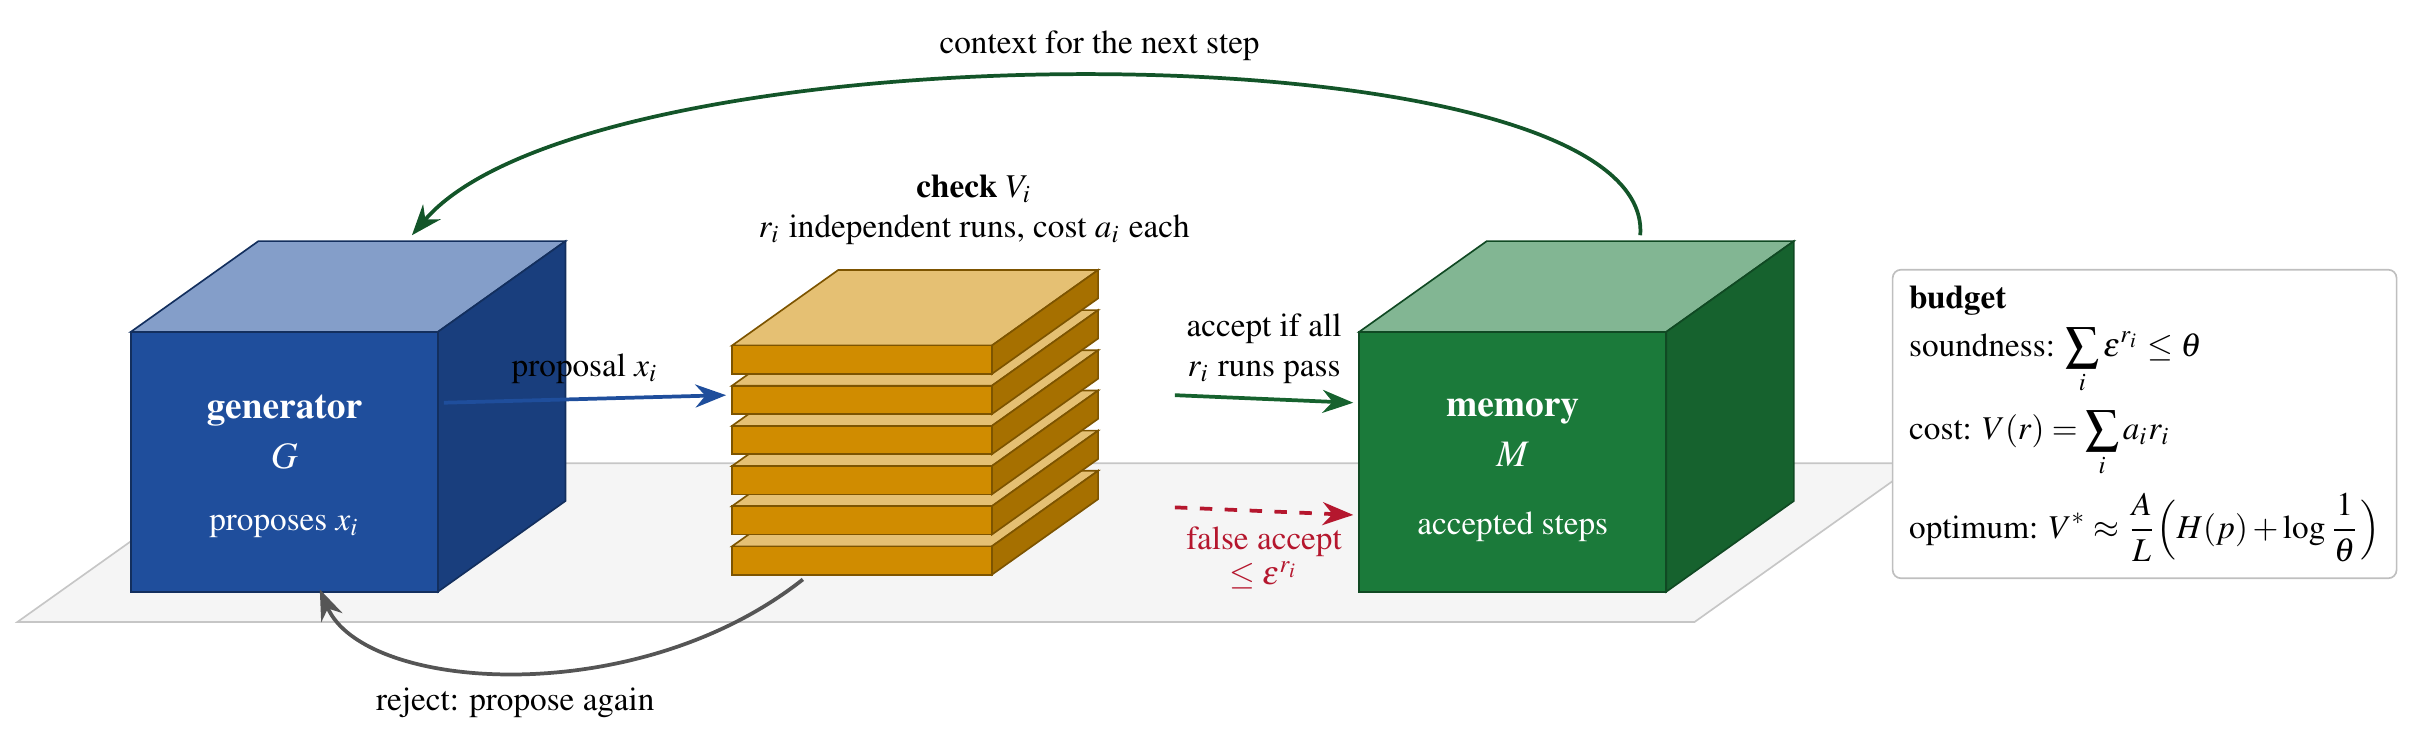
\includegraphics[width=0.94\textwidth]{figures/fig_architecture}
\caption{A BLLM. The generator proposes candidate modifications; the $i$-th candidate is tested by $r_{i}$ independent runs of a check $V_{i}$ of cost $a_{i}$ per run; an incorrect candidate survives all runs with probability at most $\eps^{r_{i}}$ and a correct one always survives; the memory keeps what survives and feeds it back as context. The budget box states the two quantities the paper controls, the expected number of false acceptances $\sum_{i}\eps^{r_{i}}\le\theta$ and the cost $V(r)=\sum_{i}a_{i}r_{i}$, and the value of the optimum (Theorem~\ref{thm:A}).}
\label{fig:architecture}
\end{figure*}

\subsection{The entropy law}

Write $A=\sum_{i}a_{i}$ for the total cost of one run of every check, $p_{i}=a_{i}/A$ for the cost profile, $H(p)=\sum_{i}p_{i}\log(1/p_{i})$ for its entropy, and $L=\log(1/\eps)$. The schedule $r$ is \emph{$\theta$-sound} when the expected number of incorrect candidates kept is at most $\theta$ in every assignment of correct and incorrect candidates, which for checks whose soundness $\eps$ is attained is the inequality $\sum_{i}\eps^{r_{i}}\le\theta$ (Section~\ref{sec:model}). Its cost is $V(r)=\sum_{i}a_{i}r_{i}$, the cost of certifying a run in which every candidate is correct, and $\Vs(\theta)$ is the least cost of a $\theta$-sound schedule.

\begin{mainthm}[Entropy law]\label{thm:A}
For $0<\theta\le1$,
\begin{equation}\label{eq:entropylaw}
\frac{A}{L}\Bigl(H(p)+\log\frac1\theta\Bigr)\ \le\ \Vs(\theta)\ \le\ \frac{A}{L}\Bigl(H(p)+\log\frac1\theta\Bigr)+A .
\end{equation}
The lower bound is attained when every $\theta p_{i}$ is an integer power of $\eps$, and the additive constant $A$ cannot be replaced by $cA$ with $c<1$. The same bounds hold for infinitely many candidates with $A<\infty$, and for schedules drawn at random independently of the checks.
\end{mainthm}

The law says that the price of soundness is an entropy. Certifying $n$ candidates of equal cost costs $(n/L)\log(n/\theta)$ up to $n$, so the tax per candidate grows like $\log n$ and not like a constant: a system that keeps more modifications must test each one harder. A skewed profile is cheaper than a flat one with the same total, because the expensive checks may be run fewer times and the cheap ones more, and the saving is measured exactly by $\log n-H(p)$. The schedule that attains the bound runs the $i$-th check $\lceil\log(A/(\theta a_{i}))/L\rceil$ times, so it spends $\log(1/p_{i})$ nats of soundness on a candidate of relative cost $p_{i}$: this is Shannon's code length \cite{Sha48}, and the analogy is exact.

\begin{mainthm}[Huffman schedules]\label{thm:C}
If $\eps=1/D$ for an integer $D\ge2$ and $\theta=D^{-k}$ for an integer $k\ge0$, then the $\theta$-sound schedules are exactly $r_{i}=\ell_{i}+k$ with $(\ell_{i})$ the lengths of a $D$-ary prefix code, and $\Vs(\theta)=A\bigl(k+L_{D}(p)\bigr)$, where $L_{D}(p)$ is the expected length of a Huffman code for $p$.
\end{mainthm}

So the optimal schedule is computed by Huffman's algorithm \cite{Huf52}, and Kraft's inequality \cite{Kra49,McM56} is the soundness condition in disguise. The additive constant of Theorem~\ref{thm:A} is the redundancy of the Huffman code, which lies in $[0,1)$ in units of $\log D$ \cite{CT06,Gal78}.

Not every check is repeated. A statistical check that averages $m$ samples and accepts when the average is close to its target has false acceptance probability of order $1/m$ by Chebyshev's inequality, not $\eps^{m}$. For a check whose cost to reach false acceptance probability $\delta$ is $a\delta^{-s}$ the entropy is replaced by a R\'enyi entropy \cite{Ren61}.

\begin{mainthm}[R\'enyi law]\label{thm:D}
For checks of polynomial order $s>0$ and $0<\theta\le1$, the least cost of a $\theta$-sound allocation is
\begin{equation}\label{eq:renyilaw}
\Vs_{s}(\theta)=\theta^{-s}\Bigl(\sum_{i}a_{i}^{1/(1+s)}\Bigr)^{1+s}=A\,\theta^{-s}e^{sH_{\alpha}(p)},
\end{equation}
where $\alpha=1/(1+s)$ and $H_{\alpha}$ is the R\'enyi entropy of order $\alpha$; and $\Vs_{s}(\theta)=A\bigl(1+s(H(p)+\log\frac1\theta)\bigr)+O(s^{2})$ as $s\to0$.
\end{mainthm}

The first-order term at $s=0$ is the entropy law, so the R\'enyi law is a one-parameter deformation of it, as Campbell's coding theorem is a deformation of Shannon's \cite{Cam65}. Section~\ref{sec:renyi} also gives a criterion, valid for every cost function, for an infinite sequence of candidates to admit a sound schedule of finite cost.

\subsection{Chains, gates and singularities}

Section~\ref{sec:chains} puts the checks into a self-improvement chain in which the generator retries a step until a candidate is kept. When each step is wrong with probability between $\rho_{\ast}>0$ and $\bar\rho<1$, the least expected cost of the chain with at most $\theta$ expected false acceptances is pinched between the entropy law at budget $\theta/\rho_{\ast}$ and the entropy law at budget $\theta(1-\bar\rho)/\bar\rho$, divided by $1-\bar\rho$ (Theorem~\ref{thm:B}). The same section proves an exponential separation between checking every step and checking only the outcome: with perfect checks the ratio of expected costs is $(1-\rho)^{-(n-1)}\ge e^{(n-1)\rho}$, and with imperfect checks the step check may accept an incorrect step with probability of order $1/n$ while the outcome check must do so with probability exponentially small in $n$ (Theorem~\ref{thm:gating}).

An infinite chain whose total expected cost is finite completes infinitely many improvements in finite cost, and we call it \emph{singular}, after the vertical asymptote of the explosion literature. It is \emph{sound} when the number $F$ of incorrect modifications it keeps is finite.

\begin{mainthm}[Sound singularities]\label{thm:E}
Let the $n$-th step cost $g_{n}$ to generate and $a_{n}\le1$ per run to check, with error probabilities in $[\rho_{\ast},\bar\rho]\subset(0,1)$, independent steps and checks of exact soundness $\eps$. Then
\begin{enumerate}[label=\textup{(\roman*)},leftmargin=2.2em,itemsep=1pt]
\item $F<\infty$ almost surely, or $\PR(F=0)>0$, if and only if $\sum_{n}\eps^{r_{n}}<\infty$, and otherwise $F=\infty$ almost surely;
\item a singular chain in which every step is checked exists if and only if $\sum_{n}g_{n}<\infty$ and $\sum_{n}a_{n}<\infty$;
\item a sound singular chain exists if and only if in addition $\sum_{n}a_{n}\log(1/a_{n})<\infty$.
\end{enumerate}
\end{mainthm}

So there is a soundness gap. For $a_{n}=1/(n\log^{\beta}n)$ a singular chain exists for every $\beta>1$, and a sound one only for $\beta>2$; between the two, every schedule fast enough to reach the asymptote keeps infinitely many errors almost surely (Corollary~\ref{cor:gap}). For a power law $a_{n}=n^{-p}$ the price of soundness, the ratio of the cheapest sound cost to the cost of one run per step, is $1/((p-1)L)+O(\log\frac1{p-1})$, and with polynomial checks of order $s$ a sound singularity exists exactly when $p>1+s$ (Fig.~\ref{fig:regimes}).

When the improvements branch, each kept improvement spawning a random number of candidates, the process is a Galton--Watson tree \cite{WG75,AN72}.

\begin{mainthm}[Branching takeoff]\label{thm:F}
Let $m$ be the mean number of correct offspring kept per kept improvement, and let the check of generation $k$ accept an incorrect candidate with probability $\delta_{k}$. Then the takeoff survives with positive probability if and only if $m>1$; the expected number of kept errors is $\mu(1-\gamma)\sum_{k\ge1}m^{k-1}\delta_{k}$; and if this series diverges then, under $\EE\,\xi\log\xi<\infty$, infinitely many errors are kept almost surely on survival. With exponential checks, soundness forces $r_{k}\ge k\log m/L$ for all large $k$, and $r_{k}=\lceil k\log(2m)/L\rceil$ suffices.
\end{mainthm}

Here $\mu$ is the mean number of candidates per kept improvement, $\gamma$ the probability that a candidate is correct and $\xi$ the number of candidates. A fixed false acceptance rate, however small, is fatal to an explosive takeoff, and the number of runs per check must grow linearly in the generation, that is, logarithmically in the size of the population: the entropy tax again.

\subsection{What the paper proves}

Table~\ref{tab:results} lists the results. The proofs are complete and elementary: the entropy law rests on the inequality $\log x\le x-1$, the R\'enyi law on H\"older's inequality, the singularity theorem on the Borel--Cantelli lemmas, and the branching theorem on the Kesten--Stigum theorem \cite{KS66} and L\'evy's conditional form of the Borel--Cantelli lemma \cite{Dur19}. Every finite inequality, the Kraft--schedule correspondence, the R\'enyi optimum, the convergence criteria for sound schedules and both Borel--Cantelli statements are proved in Lean~4 with Mathlib, in thirty-nine theorems that depend only on the three standard axioms (Appendix~\ref{app:checks}); the probabilistic limit theorems and the asymptotics of the zeta function are proved in the text and are not formalised.

The paper does not prove that any existing system is sound, and it does not predict whether an intelligence explosion will happen. Its theorems are conditional on a model, stated in Section~\ref{sec:model}: independent runs, perfect completeness, and schedules fixed in advance. Remark~\ref{rem:adaptive} shows that the last assumption matters, since a schedule allowed to stop at the first detected error escapes the entropy term at the price of discarding good work. What the paper does establish is that, inside the model, the cost of soundness is computable in closed form, that it is an entropy, and that it separates the singular processes into sound and unsound ones by a single convergent series.

\begin{table*}[t]
\caption{The main results. $A=\sum a_{i}$, $p=a/A$, $L=\log(1/\eps)$; ``Lean'' names the formalised statements of Appendix~\ref{app:checks}.}
\label{tab:results}
\centering
\footnotesize
\setlength{\tabcolsep}{4pt}
\begin{tabular}{@{}l l l >{\raggedright\arraybackslash}p{0.27\textwidth}@{}}
\toprule
Result & Statement & Proof & Lean \\
\midrule
Theorem~\ref{thm:A} & $\frac AL(H+\log\frac1\theta)\le \Vs(\theta)\le \frac AL(H+\log\frac1\theta)+A$ & Gibbs, ceilings & \lean{verification\_lower}, \lean{ceilSchedule\_cost} \\
Proposition~\ref{prop:clean} & clean runs: budgets $\theta$ and $\log\frac1{1-\theta}$ & $1-\sum q\le\prod(1-q)\le e^{-\sum q}$ & \lean{clean\_ge}, \lean{clean\_budget} \\
Proposition~\ref{prop:random} & random oblivious schedules obey Theorem~\ref{thm:A} & Jensen & \lean{randomised\_budget} \\
Proposition~\ref{prop:twosided} & two-sided checks, rate $\frac12\log\frac1{4q(1-q)}$ & Chernoff & --- \\
Theorem~\ref{thm:C} & $\Vs(D^{-k})=A(k+L_{D}(p))$ & Kraft, Huffman & \lean{kraft\_of\_schedule}, \lean{schedule\_of\_kraft} \\
Theorem~\ref{thm:D} & $\Vs_{s}(\theta)=A\theta^{-s}e^{sH_{1/(1+s)}(p)}$ & H\"older & \lean{renyi\_lower}, \lean{renyi\_attain} \\
Theorem~\ref{thm:dual} & sound schedule $\iff\sum a_{n}\psi(\lambda/a_{n})<\infty$ & Legendre duality & \lean{schedule\_of\_dual\_summable} \\
Theorem~\ref{thm:B} & chain cost between two entropy laws & Wald & \lean{entropy\_lower}, \lean{ceilSchedule\_sound} \\
Theorem~\ref{thm:gating} & step versus outcome checks: $(1-\rho)^{-(n-1)}$ & products & \lean{separation}, \lean{precision\_bounds} \\
Theorem~\ref{thm:E} & sound singularity $\iff\sum g,\sum a,\sum a\log\frac1a<\infty$ & Borel--Cantelli & \lean{sound\_schedule\_iff}, \lean{false\_accepts\_infinite} \\
Corollary~\ref{cor:gap} & soundness gap $1<\beta\le2$ & condensation & --- \\
Proposition~\ref{prop:powerlaw} & price $\sim1/((p-1)L)$ for $a_{n}=n^{-p}$ & integral comparison & --- \\
Proposition~\ref{prop:osgood} & Osgood takeoff: check time $\asymp\kappa/(c(\alpha-1)^{2}L)$ & entropy of $\zeta$ & --- \\
Theorem~\ref{thm:F} & branching takeoff and $r_{k}\ge k\log m/L$ & Kesten--Stigum, L\'evy & \lean{amplified\_summable}, \lean{contamination\_diverges} \\
\bottomrule
\end{tabular}
\end{table*}

\subsection{Organisation}

Section~\ref{sec:history} traces the three lines that meet here: self-reference and the intelligence explosion, coding and testing, and branching processes, together with the recent work on verifiers for language models. Section~\ref{sec:model} defines the model. Sections~\ref{sec:entropy} to~\ref{sec:renyi} prove the entropy law, its Huffman form and its R\'enyi deformation, with the duality criterion for infinite sequences. Section~\ref{sec:chains} treats chains and the comparison of step and outcome checks, Section~\ref{sec:singularity} the singular chains, Section~\ref{sec:branching} the branching takeoff, and Section~\ref{sec:scaling} relates the cost sequences to growth laws and to the empirical scaling laws of language models. Section~\ref{sec:status} states what is proved and what remains open. Appendix~\ref{app:derivations} collects the classical facts used, with proofs, and Appendix~\ref{app:checks} the Lean statements and the numerical checks.

Logarithms are natural unless a base is shown; $\NN=\{0,1,2,\dots\}$.

\section{History}\label{sec:history}

Three lines of work meet in this paper, and a fourth, recent one supplies its motivation. Figure~\ref{fig:history} places them on one time axis and Table~\ref{tab:history} lists what each contributes to the argument.

\begin{figure*}[t]
\centering
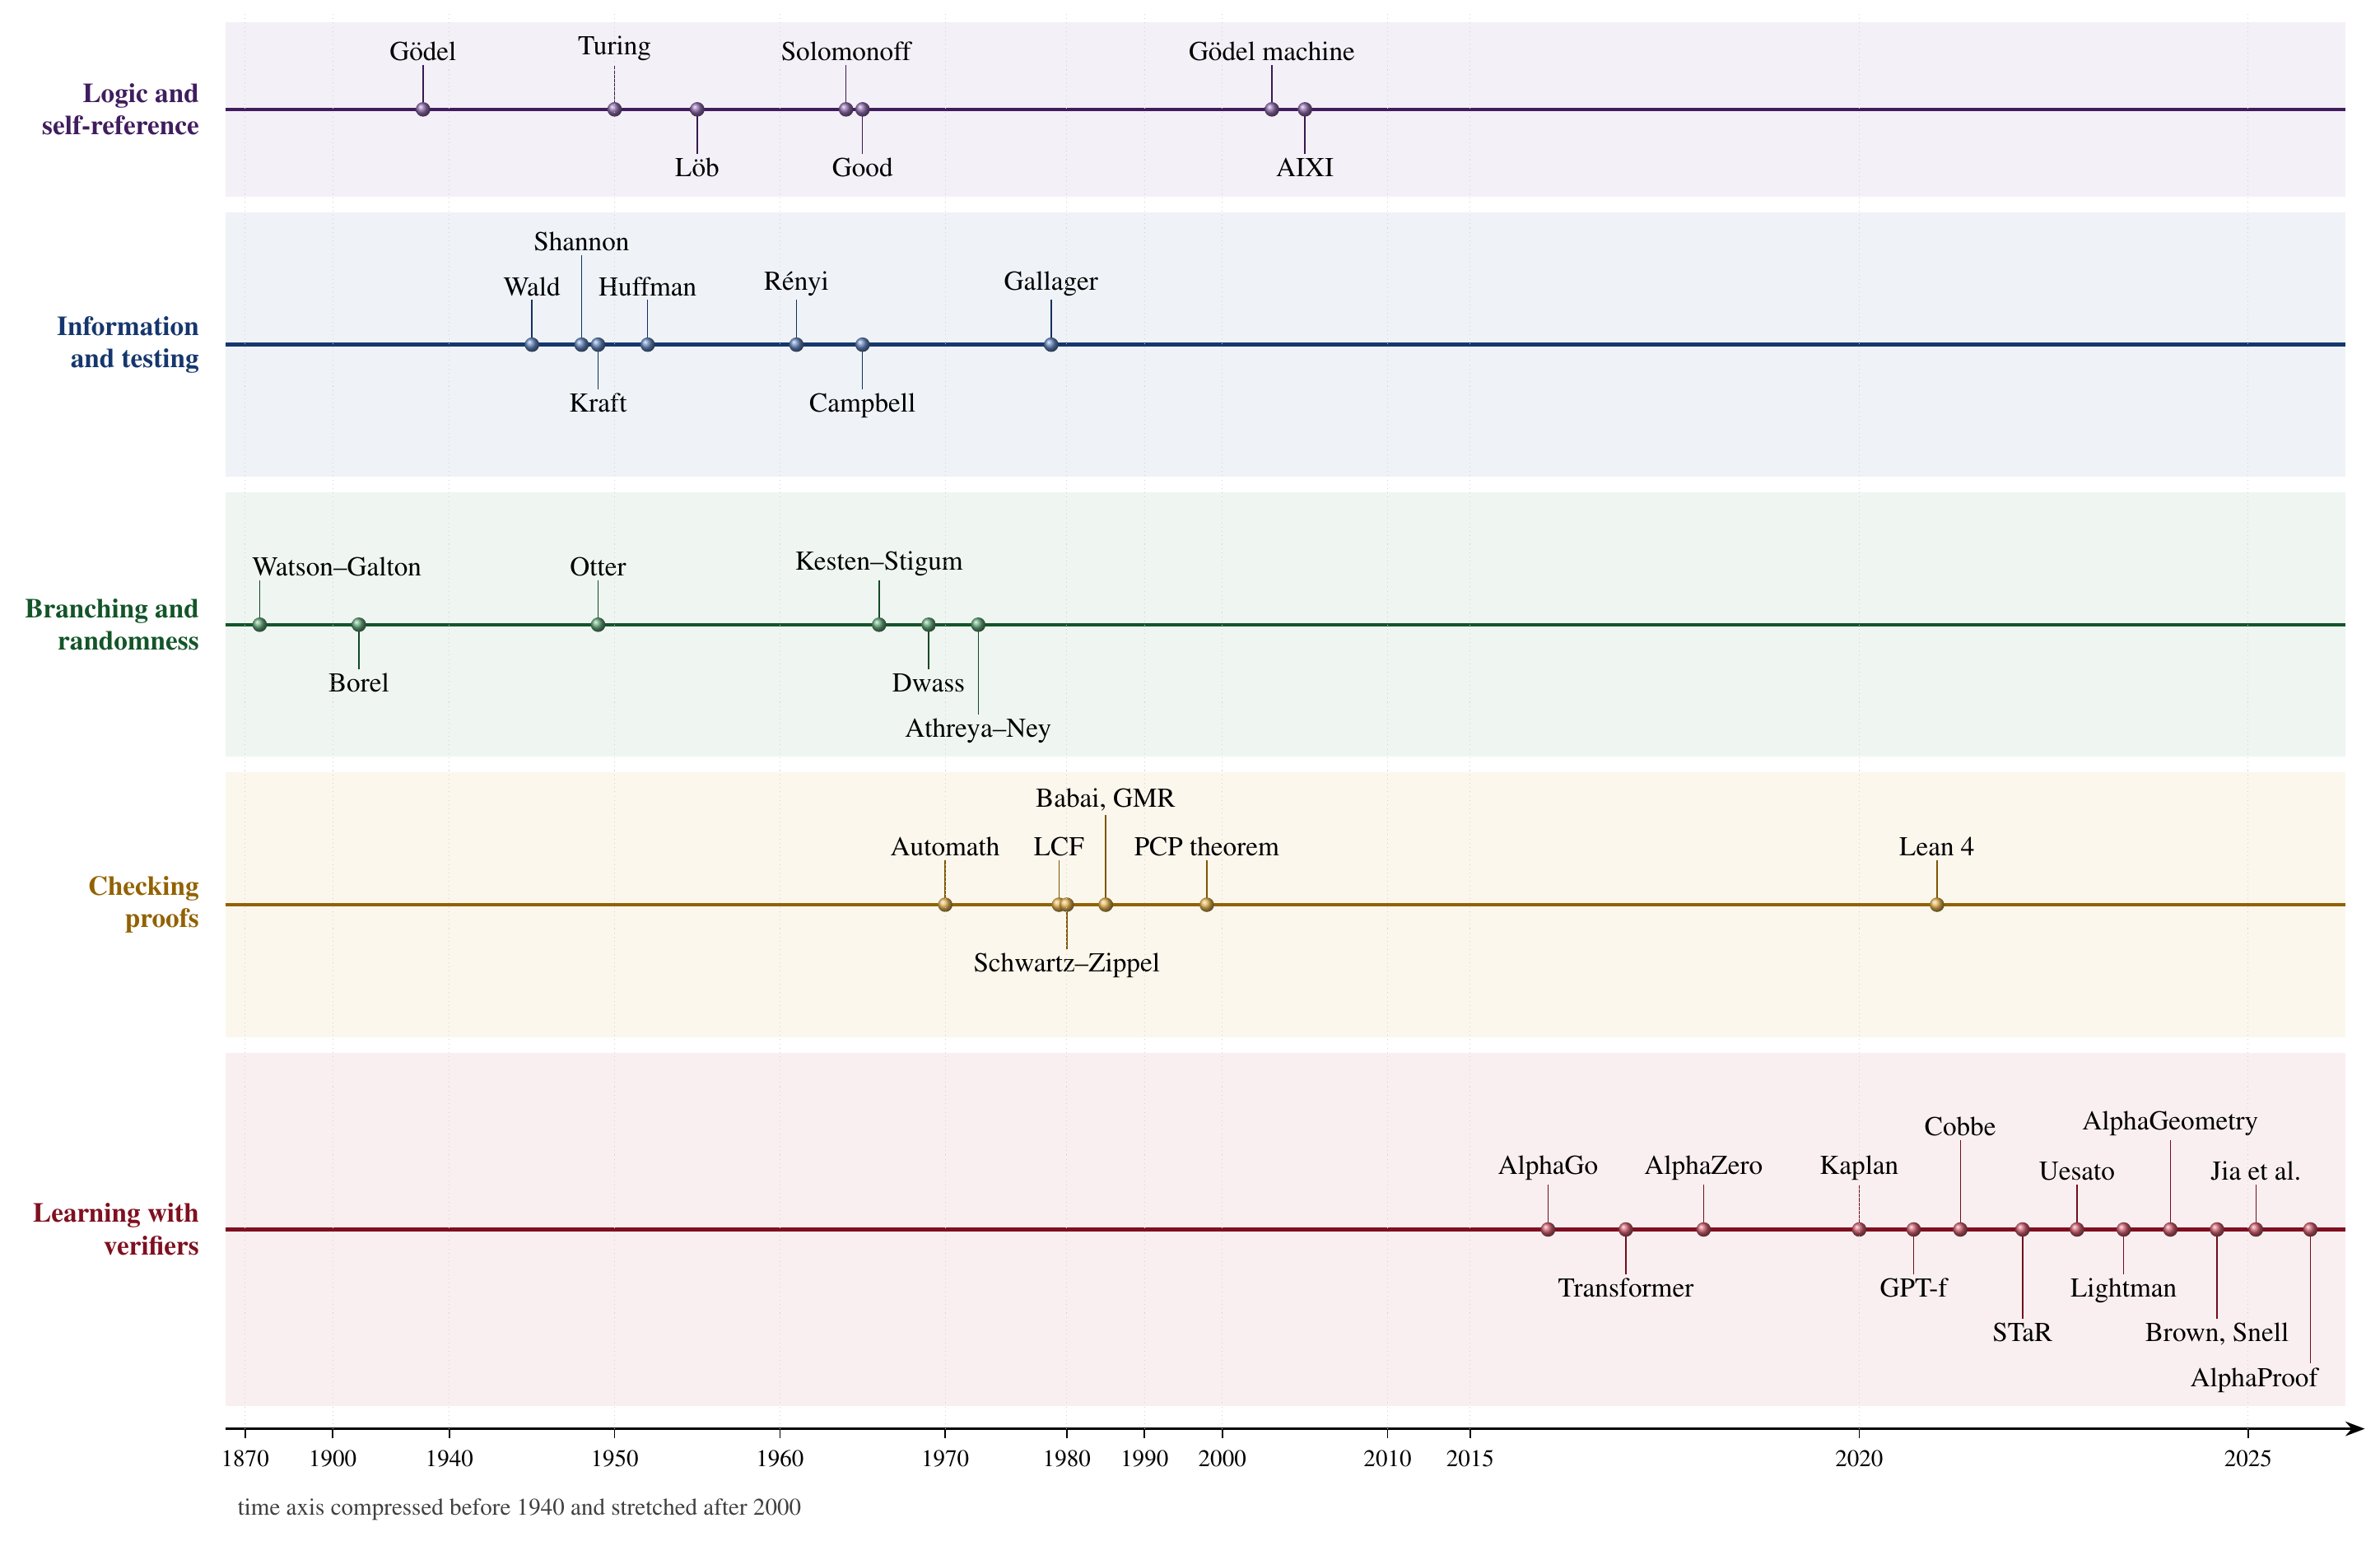
\includegraphics[width=\textwidth]{figures/fig_history}
\caption{Five lines of work on one time axis, with the scale stretched after 2015. Logic and self-reference: G\"odel's incompleteness theorems, Turing's learning machine, L\"ob's theorem, Solomonoff's induction, Good's intelligence explosion, the G\"odel machine and AIXI. Information and testing: Wald's sequential tests, Shannon's source coding, Kraft's inequality, Huffman's codes, R\'enyi's entropies, Campbell's coding theorem and Gallager's redundancy bound. Branching and randomness: the Watson--Galton problem, Borel's denumerable probabilities, Otter's multiplicative process, the Kesten--Stigum theorem, Dwass's total progeny and the monograph of Athreya and Ney. Checking proofs: Automath, LCF, the polynomial identity test of Schwartz and Zippel, interactive proofs, the PCP theorem and Lean~4. Learning with verifiers: from AlphaGo and the transformer to trained verifiers, process supervision, repeated sampling and AlphaProof.}
\label{fig:history}
\end{figure*}

\subsection{Self-reference and the intelligence explosion}

Turing's paper of 1950 already contains the idea of a machine that improves itself: rather than program an adult mind, one should program a child machine and educate it, and he expected the educated machine to be modified by its own experience \cite{Tur50}. Fifteen years later Good drew the consequence for machines better than their designers \cite{Goo66}. The formal theory of such machines met an obstacle at once, and the obstacle is logical. G\"odel's second incompleteness theorem shows that a consistent system containing arithmetic does not prove its own consistency \cite{God31}, and L\"ob's theorem sharpens it: if such a system proves that provability of a sentence implies the sentence, then it proves the sentence \cite{Lob55}.\footnote{L\"ob's theorem answers a question of Henkin. Let $T$ be a consistent recursively axiomatised extension of Peano arithmetic and $\mathrm{Prov}_{T}$ its provability predicate. If $T\vdash\mathrm{Prov}_{T}(\ulcorner\varphi\urcorner)\to\varphi$ then $T\vdash\varphi$. Applied to a self-modifying agent that keeps a successor only when it proves the successor sound, the theorem forbids the agent from accepting, in general, a successor that uses the same proof system with the same trust, since that acceptance would require the agent to prove a reflection principle for its own system. The present paper avoids the obstacle by replacing proofs of soundness with randomized checks of bounded error, whose reliability is a probability, not a theorem of the system.} An agent that rewrites itself only after proving that the rewrite is sound cannot in general accept a successor as strong as itself. Schmidhuber's G\"odel machine makes this precise in the other direction: it rewrites any part of its own code once it has found a proof that the rewrite increases expected utility, and is optimal among such strategies relative to its axioms \cite{Sch03}. Solomonoff's theory of inductive inference \cite{Sol64} and Hutter's AIXI \cite{Hut05} give the ideal, uncomputable agents against which the practical ones are measured.

The present paper does not ask for proofs. It asks for checks with a stated probability of error and counts what they cost. That shift, from certainty to bounded error, is the one complexity theory made between the 1970s and the 1990s.

\subsection{Coding and testing}

Shannon's theorem of 1948 says that a source with distribution $p$ cannot be encoded by a uniquely decodable code in fewer than $H(p)$ symbols on average, and that $H(p)+1$ can be reached \cite{Sha48}. Kraft's inequality, from his master's thesis of 1949, characterises the lengths of prefix codes \cite{Kra49}; McMillan extended it to all uniquely decodable codes \cite{McM56}; Huffman's algorithm of 1952 finds an optimal code \cite{Huf52}; Gallager bounded its redundancy \cite{Gal78}. R\'enyi introduced in 1961 a family of entropies $H_{\alpha}$ that share the additivity of Shannon's \cite{Ren61}, and Campbell showed in 1965 that $H_{\alpha}$ is the optimal mean length when long codewords are penalised exponentially \cite{Cam65}. The standard account is \cite{CT06}.

The connection with checking is older than it looks. Wald's sequential tests of 1945 already treat the trade-off between the number of observations and the two probabilities of error \cite{Wal45}, and Chernoff's exponent of 1952 \cite{Che52} and Hoeffding's inequality of 1963 \cite{Hoe63} give the rates at which repeated observations drive the error down. What seems not to have been noticed is that the optimal allocation of repetitions among many checks of unequal cost under a common error budget is a coding problem, with costs in the role of probabilities and repetitions in the role of codeword lengths. Theorems~\ref{thm:A} and~\ref{thm:C} make the identification exact.

\subsection{Branching and randomness}

The Watson--Galton paper of 1875 asked for the probability that a surname dies out, and reduced the question to the iteration of a generating function \cite{WG75}; the conclusion drawn there, that every family dies out, was wrong, and the correct criterion, extinction with probability one exactly when the mean number of sons is at most one, became standard only in the twentieth century. Otter's multiplicative process of 1949 put the theory in its modern form \cite{Ott49}, Kesten and Stigum proved in 1966 that the normalised population converges to a limit that is positive on survival exactly when $\EE\,\xi\log\xi<\infty$ \cite{KS66}, and Dwass related the total progeny to a random walk \cite{Dwa69}; the monograph of Athreya and Ney is the reference \cite{AN72}. Borel's paper of 1909 on denumerable probabilities contains the first form of the Borel--Cantelli lemma \cite{Bor09}, which decides here whether a sound singular chain keeps finitely many errors. Osgood's criterion of 1898 for blow-up of the equation $y'=f(y)$ \cite{Osg98} is the continuous form of the condition $\sum a_{n}<\infty$ for a singularity.

\subsection{Checking proofs}

De Bruijn's Automath \cite{dB70} and Milner's LCF \cite{GMW79} began the mechanical checking of proofs, and Lean~4 \cite{MU21} is the system used here. In parallel, complexity theory replaced certainty by bounded error. Schwartz and Zippel showed that a polynomial identity can be tested by evaluating at random points, with error at most the degree divided by the size of the field per run \cite{Sch80,Zip79}; Babai \cite{Bab85} and Goldwasser, Micali and Rackoff \cite{GMR89} introduced interactive proofs, in which a verifier is convinced with error probability that halves with each round; the PCP theorem showed that every proof can be written so that a verifier reads a constant number of its bits and errs with probability at most one half \cite{AS98,ALM98}. These are exactly the checks of the present paper: perfect completeness, soundness $\eps<1$ per run, and independent repetition.

\subsection{Learning with verifiers}

The fourth line is recent. AlphaGo \cite{SHM16} and AlphaZero \cite{SHS18} learned games by self-play against an exact referee, the rules of the game. Transformers \cite{VSP17} and the scaling of language models \cite{BMR20,KMH20,HBM22} produced generators of proofs and programs, and verifiers were added to them: Polu and Sutskever coupled a language model to the Metamath checker \cite{PS20}, Cobbe and coauthors trained verifiers to rank solutions of arithmetic problems \cite{CKB21}, Uesato and coauthors and Lightman and coauthors compared rewards for the final answer with rewards for every step \cite{UKK22,LKB23}, and chains of thought made the steps explicit \cite{WWS22}. Self-improvement loops followed: a model trained on its own checked rationales \cite{ZWM22}, on its own consistent answers \cite{HGH22}, on its own feedback \cite{MTG23} or on a constitution \cite{BKK22}. Spending computation at inference time, by sampling many candidates and keeping the checked ones, became a lever of its own \cite{BJE24,SLX24}. AlphaGeometry \cite{TWL24} and AlphaProof \cite{HMS25} reached olympiad level by searching against exact checkers. Errors of transformers on compositional tasks grow with the number of steps \cite{DLS23}, which is one reason to check every step.

The theory has followed. Jia, Rakhlin and Xie showed that learning from outcome supervision is statistically no harder than learning from process supervision, up to polynomial factors in the horizon \cite{JRX25}; Botta and coauthors showed that a process verifier can turn an intractable generation problem into a tractable one \cite{BLM25}; Rohatgi and coauthors showed that small errors of a learned verifier are amplified along a generation and designed a backtracking sampler that resists them \cite{RSS25}; Balcan and coauthors studied learned verifiers of chains of thought and the asymmetric role of their soundness errors \cite{BBF26}; Scrivens reported that classifier-based safety gates fail over many rounds of self-improvement while a verifier with analytic bounds does not \cite{Scr26}; Guo turned impossibility results into design rules \cite{Guo26}; Lu compared improvements of agentic systems through bounded verification and showed that independent majority amplification preserves the languages it defines \cite{Lu26}. On the growth side, Ord showed that singular growth requires the time around the feedback loop to tend to zero \cite{Ord26}, Anbar Jafari, Ozcinar and Anbarjafari gave testable conditions for runaway growth \cite{AOA25}, and the first author with Singha Roy and Samal studied phase transitions and predictability limits of general intelligence \cite{BSS26}. The verifier-gated engine of \cite{Bha26a} and the earlier analysis of the expulsion of a superintelligence from human control \cite{Bha21} are the two works of the first author on which the present architecture is built.

None of these works prices soundness. They bound sample complexity, query complexity, error amplification or growth rates, and they treat the verifier as given. The question here is how a fixed budget of false acceptances should be distributed over many checks of different costs, and what that distribution costs; the answer is an entropy, and it decides which singular takeoffs are sound.

\begin{table*}[t]
\caption{Milestones used in the paper. The last column says where each enters the argument.}
\label{tab:history}
\centering
\small
\begin{tabular}{@{}l l p{0.42\textwidth} l@{}}
\toprule
Year & Work & Contribution & Used in \\
\midrule
1875 & Watson, Galton \cite{WG75} & extinction of families by iterating a generating function & Theorem~\ref{thm:F} \\
1898 & Osgood \cite{Osg98} & blow-up of $y'=f(y)$ in finite time & Section~\ref{sec:scaling} \\
1909 & Borel \cite{Bor09} & denumerable probabilities, Borel--Cantelli & Theorem~\ref{thm:E} \\
1931, 1955 & G\"odel, L\"ob \cite{God31,Lob55} & limits of self-trust in formal systems & Section~\ref{sec:history} \\
1945 & Wald \cite{Wal45} & sequential tests and two probabilities of error & Section~\ref{ssec:twosided} \\
1948 & Shannon \cite{Sha48} & entropy as the optimal mean code length & Theorem~\ref{thm:A} \\
1949, 1956 & Kraft, McMillan \cite{Kra49,McM56} & lengths of prefix and decodable codes & Theorem~\ref{thm:C} \\
1949 & Otter \cite{Ott49} & multiplicative processes & Theorem~\ref{thm:F} \\
1952 & Huffman \cite{Huf52} & optimal prefix codes & Theorem~\ref{thm:C} \\
1952 & Chernoff \cite{Che52} & exponential rate of tests on sums & Proposition~\ref{prop:twosided} \\
1961, 1965 & R\'enyi, Campbell \cite{Ren61,Cam65} & entropies of order $\alpha$ and exponential code costs & Theorem~\ref{thm:D} \\
1965 & Good \cite{Goo66} & the intelligence explosion & Section~\ref{sec:intro} \\
1966 & Kesten, Stigum \cite{KS66} & the limit $Z_{k}/m^{k}$ on survival & Theorem~\ref{thm:F} \\
1979--1980 & Schwartz, Zippel \cite{Sch80,Zip79} & randomized identity tests with one-sided error & Section~\ref{sec:model} \\
1985--1998 & Babai; GMR; PCP \cite{Bab85,GMR89,AS98,ALM98} & bounded-error verification of proofs & Section~\ref{sec:model} \\
2003 & Schmidhuber \cite{Sch03} & self-rewriting after a proof of improvement & Section~\ref{sec:history} \\
2021--2023 & Cobbe; Uesato; Lightman \cite{CKB21,UKK22,LKB23} & trained verifiers, process and outcome rewards & Theorem~\ref{thm:gating} \\
2024--2025 & AlphaGeometry, AlphaProof \cite{TWL24,HMS25} & search against exact checkers & Section~\ref{sec:model} \\
2025--2026 & Jia et al.; Rohatgi et al.; Ord \cite{JRX25,RSS25,Ord26} & outcome supervision, verifier errors, singular growth & Sections~\ref{sec:chains}, \ref{sec:scaling} \\
\bottomrule
\end{tabular}
\end{table*}

\section{The model}\label{sec:model}

\subsection{Checks}

A \emph{candidate} is a proposed modification of the system: an edit of its weights, a patch of its code, a new lemma in its library, a step of a proof. It is either correct or incorrect, and nothing in the model depends on what the two words mean, only on the fact that the check can tell them apart with one-sided error.

\begin{definition}[Check]\label{def:check}
A \emph{check} for a candidate is a randomized procedure that outputs \emph{accept} or \emph{reject}. A \emph{run} of the check uses fresh randomness, so that runs on the same candidate are independent. The check has \emph{perfect completeness} if it accepts a correct candidate with probability one, and \emph{soundness} $\eps\in(0,1)$ if it accepts an incorrect candidate with probability at most $\eps$ in each run. It is \emph{sharp} if the probability is exactly $\eps$ for every incorrect candidate. A run of the check of candidate $i$ costs $a_{i}>0$.
\end{definition}

The Schwartz--Zippel test of a polynomial identity of degree $d$ over a field with $q$ elements is a check of soundness $d/q$ \cite{Sch80,Zip79}; a round of an interactive proof with soundness one half is a check of soundness $1/2$ \cite{Bab85,GMR89}; a PCP verifier is a check of soundness $1/2$ that reads a constant number of bits \cite{AS98,ALM98}; a search for a counterexample that succeeds with probability at least $1-\eps$ on every incorrect candidate is a check of soundness $\eps$. A proof checker such as Lean \cite{MU21} is a check of soundness zero, and the model applies to it with $\eps$ replaced by the probability that the randomized search that produces the certificate misses an error the checker would detect. Checks need not be classical: the only property used is the independence of runs, which holds as well for repeated preparation and measurement in the quantum procedures of \cite{Bha26b,SBS26}.\footnote{Independence is the one structural assumption. If the $r$ runs of a check on an incorrect candidate pass together with probability $\kappa^{-1}(r)$ for some decreasing function, the analysis of Section~\ref{sec:renyi} applies with the cost function $\kappa$ in place of the exponential one, and Theorem~\ref{thm:dual} gives the criterion for an infinite sequence of candidates. Correlated runs of a learned verifier, for example several samples of a reward model on the same input, are of this kind.}

\subsection{Schedules, soundness and cost}

There are $n$ candidates, indexed by $i$, or infinitely many, indexed by $n\ge1$. A \emph{world} $w$ is an assignment of the labels correct and incorrect to the candidates; it is arbitrary and unknown. A \emph{schedule} is a vector $r=(r_{i})$ of nonnegative integers fixed before any check runs. The protocol runs the check of candidate $i$ at most $r_{i}$ times, stops at the first rejection, and keeps the candidate if all $r_{i}$ runs accept; a candidate with $r_{i}=0$ is kept unchecked. The decisions on different candidates use independent randomness.

\begin{definition}[Soundness and cost of a schedule]\label{def:sound}
Let $F$ be the number of incorrect candidates kept. The schedule is \emph{$\theta$-sound} if $\EE_{w}F\le\theta$ in every world $w$. Its \emph{cost} is $V(r)=\sum_{i}a_{i}r_{i}$, and
\[
\Vs(\theta)=\inf\Bigl\{V(r)\colon r\in\NN^{n},\ \sum_{i}\eps^{r_{i}}\le\theta\Bigr\}.
\]
\end{definition}

\begin{lemma}\label{lem:sound}
Let every check have perfect completeness and soundness $\eps$.
\begin{enumerate}[label=\textup{(\roman*)},leftmargin=2.2em,itemsep=1pt]
\item If $\sum_{i}\eps^{r_{i}}\le\theta$, then $r$ is $\theta$-sound, and $\PR_{w}(F\ge1)\le\theta$ in every world.
\item If the checks are sharp and $r$ is $\theta$-sound, then $\sum_{i}\eps^{r_{i}}\le\theta$.
\item In every world and for every outcome of the checks, the cost of the protocol is at most $V(r)$, with equality in the world in which every candidate is correct.
\end{enumerate}
\end{lemma}

\begin{proof}
An incorrect candidate $i$ is kept when its $r_{i}$ independent runs all accept, which has probability at most $\eps^{r_{i}}$, with equality for a sharp check. By linearity of expectation $\EE_{w}F\le\sum_{i\text{ incorrect in }w}\eps^{r_{i}}\le\sum_{i}\eps^{r_{i}}$, and $\PR_{w}(F\ge1)\le\EE_{w}F$. In the world in which every candidate is incorrect and the checks are sharp, $\EE_{w}F=\sum_{i}\eps^{r_{i}}$, which proves (ii). The protocol spends at most $r_{i}$ runs on candidate $i$, and exactly $r_{i}$ when the candidate is correct, since a correct candidate is never rejected.
\end{proof}

So for sharp checks $\Vs(\theta)$ is the least cost of a $\theta$-sound schedule, and for checks whose soundness is only bounded it is the least cost of a schedule that is $\theta$-sound by the union bound. The cost $V(r)$ is the cost of the run the system exists to produce, one in which every candidate it keeps is correct, and it is also the largest cost the protocol can incur. The set of schedules of cost at most any given value is finite, because $a_{i}>0$, so the infimum is a minimum when $n$ is finite.

\begin{definition}[Profile]\label{def:profile}
For finitely many candidates, or for infinitely many with $A=\sum a_{i}<\infty$, the \emph{cost profile} is $p_{i}=a_{i}/A$ and its \emph{entropy} is $H(p)=\sum_{i}p_{i}\log(1/p_{i})\in[0,\infty]$. Write $L=\log(1/\eps)>0$.
\end{definition}

For $n$ candidates $0\le H(p)\le\log n$, with $H(p)=\log n$ exactly for equal costs; for infinitely many, $H(p)$ may be infinite even when $A$ is finite, and Section~\ref{sec:singularity} turns on this possibility. The identity
\begin{equation}\label{eq:AH}
A\,H(p)=\sum_{i}a_{i}\log\frac{A}{a_{i}}=\sum_{i}a_{i}\log\frac1{a_{i}}+A\log A
\end{equation}
is used throughout.

\subsection{Three assumptions}

The model makes three assumptions, and each is tested in the paper. Independence of runs is relaxed in Section~\ref{sec:renyi}, where the cost of reaching false acceptance probability $\delta$ is an arbitrary function. Perfect completeness is relaxed in Section~\ref{ssec:twosided}, where both kinds of error occur and the decision is a majority vote. The schedule fixed in advance is the assumption that cannot be removed without changing the answer: Remark~\ref{rem:adaptive} shows that a protocol allowed to stop the whole run at the first rejection escapes the entropy term. Fixed schedules are natural for a BLLM, which allots a verification budget to each modification before it sees the outcome, and they are the only ones under which the decision on a candidate depends on that candidate alone.

\section{The entropy law}\label{sec:entropy}

\subsection{Two inequalities}

Everything in this section rests on $\log x\le x-1$ for $x>0$, with equality only at $x=1$.

\begin{lemma}[Gibbs term]\label{lem:gibbs}
For $x,y>0$, $x\log(1/x)\le x\log(1/y)+y-x$, with equality if and only if $x=y$.
\end{lemma}

\begin{proof}
Apply $\log t\le t-1$ to $t=y/x$ and multiply by $x$: $x\log y-x\log x\le y-x$.
\end{proof}

\begin{lemma}[Entropy term]\label{lem:entropyterm}
For $a,b,A,\theta>0$,
\[
a\log\frac Aa+a\log\frac1\theta\ \le\ a\log\frac1b+\frac{Ab}{\theta}-a,
\]
with equality if and only if $b=\theta a/A$.
\end{lemma}

\begin{proof}
Apply $\log t\le t-1$ to $t=Ab/(\theta a)$, so that $\log A+\log b-\log\theta-\log a\le Ab/(\theta a)-1$, and multiply by $a$.
\end{proof}

\begin{proposition}[Entropy inequality]\label{prop:entropyineq}
Let $a_{1},\dots,a_{n}>0$ with sum $A$, let $\beta_{1},\dots,\beta_{n}>0$ and $\theta>0$ with $\sum_{i}\beta_{i}\le\theta$. Then
\begin{equation}\label{eq:entropyineq}
A\,H(p)+A\log\frac1\theta\ \le\ \sum_{i}a_{i}\log\frac1{\beta_{i}},
\end{equation}
with equality if and only if $\beta_{i}=\theta p_{i}$ for every $i$.
\end{proposition}

\begin{proof}
Sum Lemma~\ref{lem:entropyterm} with $(a,b)=(a_{i},\beta_{i})$. By \eqref{eq:AH} the left side is $AH(p)+A\log(1/\theta)$, and the right side is $\sum_{i}a_{i}\log(1/\beta_{i})+(A/\theta)\sum_{i}\beta_{i}-A\le\sum_{i}a_{i}\log(1/\beta_{i})$. Equality forces equality in every term and $\sum_{i}\beta_{i}=\theta$, that is $\beta_{i}=\theta a_{i}/A$.
\end{proof}

The inequality says that among all ways of spending a budget $\theta$ of false acceptances on $n$ items, the weighted sum of the ``surprisals'' $\log(1/\beta_{i})$ is least when the budget is shared in proportion to the costs. It is Gibbs' inequality for the probability vectors $p$ and $\beta/\theta$, with a slack $\theta-\sum\beta_{i}$ that only helps.

\subsection{Proof of the entropy law}

\begin{proof}[Proof of Theorem~\ref{thm:A}]
We treat finitely many candidates; the infinite case is Proposition~\ref{prop:infinite}.

\emph{Lower bound.} Let $r$ satisfy $\sum_{i}\eps^{r_{i}}\le\theta$ and put $\beta_{i}=\eps^{r_{i}}>0$. Then $\log(1/\beta_{i})=r_{i}L$, and Proposition~\ref{prop:entropyineq} gives
\[
AH(p)+A\log\frac1\theta\ \le\ L\sum_{i}a_{i}r_{i}=L\,V(r).
\]
Dividing by $L$ and taking the minimum over $r$ gives the left inequality of \eqref{eq:entropylaw}.

\emph{Upper bound.} Let $r_{i}=\lceil x_{i}\rceil$ with $x_{i}=\log(A/(\theta a_{i}))/L$. Since $\theta\le1$ and $a_{i}\le A$, $x_{i}\ge0$, so $x_{i}\le r_{i}<x_{i}+1$. The first inequality gives $\eps^{r_{i}}\le\eps^{x_{i}}=\theta a_{i}/A$, hence $\sum_{i}\eps^{r_{i}}\le\theta$. The second gives
\[
V(r)<\sum_{i}a_{i}\Bigl(\frac1L\log\frac{A}{\theta a_{i}}+1\Bigr)=\frac AL\Bigl(H(p)+\log\frac1\theta\Bigr)+A .
\]

\emph{Equality.} If $\theta p_{i}=\eps^{k_{i}}$ with $k_{i}\in\NN$, the schedule $r_{i}=k_{i}$ has $\sum\eps^{r_{i}}=\theta\sum p_{i}=\theta$ and $V(r)=\sum_{i}a_{i}\log(1/(\theta p_{i}))/L=(A/L)(H(p)+\log(1/\theta))$.

\emph{The constant $A$.} Take $\eps=\frac12$, $\theta=1$, $n=2$ and $a=(1-t,t)$ with $0<t<\frac12$. A schedule with $r_{1}=0$ or $r_{2}=0$ has $\sum2^{-r_{i}}>1$, so every feasible schedule has $r_{1},r_{2}\ge1$, and $r=(1,1)$ is feasible; hence $\Vs(1)=A=1$. The lower bound is $H(p)/\log2$, which tends to $0$ as $t\to0$. So the gap $\Vs-(A/L)(H+\log\frac1\theta)$ approaches $A$, and no constant $cA$ with $c<1$ bounds it.
\end{proof}

Figure~\ref{fig:schedule} shows the ceiling schedule for a power-law profile and compares its cost with the lower bound over twelve decades of $\theta$.

\begin{figure*}[t]
\centering
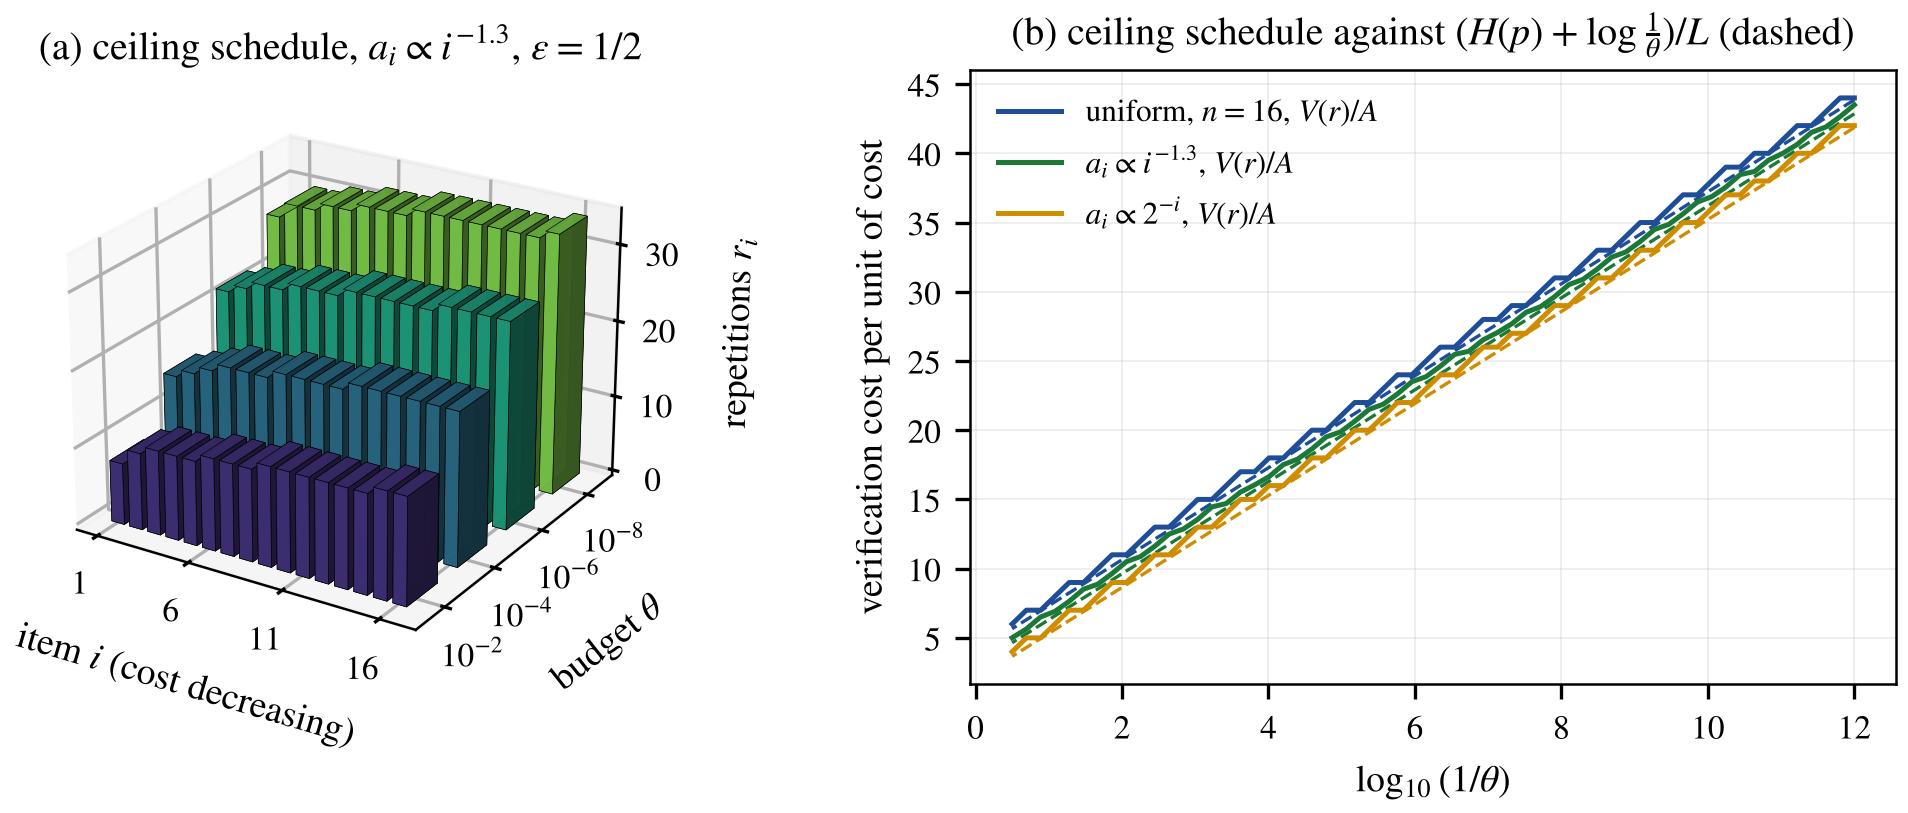
\includegraphics[width=0.98\textwidth]{figures/fig_schedule3d}
\caption{The entropy law. (a) The ceiling schedule $r_{i}=\lceil\log_{2}(A/(\theta a_{i}))\rceil$ for sixteen candidates with costs $a_{i}\propto i^{-1.3}$ and $\eps=\frac12$, at the budgets $\theta=10^{-2}$, $10^{-4}$, $10^{-6}$, $10^{-8}$: the expensive candidates receive the fewest runs, and each factor $100$ of $\theta$ adds six or seven runs to every check. (b) The cost of the ceiling schedule divided by $A$, for the uniform profile on sixteen candidates and the profiles $a_{i}\propto i^{-1.3}$ and $a_{i}\propto2^{-i}$ on sixteen, against the lower bound $(H(p)+\log\frac1\theta)/L$ (dashed). The curves stay in the band of width one above the bound, as Theorem~\ref{thm:A} asserts, and the more skewed the profile the lower the line.}
\label{fig:schedule}
\end{figure*}

\begin{corollary}[Equal costs]\label{cor:uniform}
For $n$ candidates of cost $a$ each, $\frac{na}{L}\log\frac n\theta\le\Vs(\theta)\le\frac{na}{L}\log\frac n\theta+na$. In particular the number of runs per candidate in an optimal schedule is $\log(n/\theta)/L+O(1)$.
\end{corollary}

\begin{proof}
Here $A=na$ and $H(p)=\log n$.
\end{proof}

\begin{proposition}[Shape of the optimum]\label{prop:shape}
Every optimal schedule is antitone in the costs: if $a_{i}>a_{j}$ then $r_{i}\le r_{j}$. The real relaxation, the minimum of $\sum a_{i}x_{i}$ over $x\in[0,\infty)^{n}$ with $\sum\eps^{x_{i}}\le\theta$, is attained only at $x_{i}=\log(A/(\theta a_{i}))/L$ and equals the lower bound of \eqref{eq:entropylaw}.
\end{proposition}

\begin{proof}
If $a_{i}>a_{j}$ and $r_{i}>r_{j}$, exchanging $r_{i}$ and $r_{j}$ keeps $\sum\eps^{r}$ and lowers the cost by $(a_{i}-a_{j})(r_{i}-r_{j})>0$, so $r$ was not optimal. For the relaxation, Proposition~\ref{prop:entropyineq} with $\beta_{i}=\eps^{x_{i}}$ gives $\sum a_{i}x_{i}\ge(A/L)(H+\log\frac1\theta)$, with equality exactly when $\eps^{x_{i}}=\theta p_{i}$.
\end{proof}

The marginal price of soundness is constant: lowering $\theta$ by a factor $e$ raises the lower bound by $A/L$, one nat of soundness bought on every check.

\begin{corollary}[Checks of different soundness]\label{cor:hetero}
If the check of candidate $i$ has soundness $\eps_{i}$, put $L_{i}=\log(1/\eps_{i})$, $b_{i}=a_{i}/L_{i}$, $B=\sum b_{i}$ and $q=b/B$. Then the least cost of a schedule with $\sum\eps_{i}^{r_{i}}\le\theta$, for $0<\theta\le1$, lies between $B(H(q)+\log\frac1\theta)$ and $B(H(q)+\log\frac1\theta)+A$.
\end{corollary}

\begin{proof}
The cost is $\sum a_{i}r_{i}=\sum b_{i}(r_{i}L_{i})$ and $\eps_{i}^{r_{i}}=e^{-r_{i}L_{i}}$. Proposition~\ref{prop:entropyineq} with weights $b_{i}$ and $\beta_{i}=e^{-r_{i}L_{i}}$ gives the lower bound, and $r_{i}=\lceil\log(B/(\theta b_{i}))/L_{i}\rceil$ gives $\sum\eps_{i}^{r_{i}}\le\theta\sum b_{i}/B=\theta$ and cost below $\sum b_{i}\log(B/(\theta b_{i}))+\sum a_{i}$.
\end{proof}

So the right unit of cost is the cost of one nat of soundness, $a_{i}/L_{i}$, and the entropy is that of the profile measured in this unit.

\subsection{Infinitely many candidates}

\begin{proposition}\label{prop:infinite}
Let $(a_{n})_{n\ge1}$ be positive with $A=\sum a_{n}<\infty$, and let $\Vs(\theta)$ be the infimum of $\sum a_{n}r_{n}$ over $r\in\NN^{\NN}$ with $\sum\eps^{r_{n}}\le\theta$. Then \eqref{eq:entropylaw} holds for $0<\theta\le1$, with both sides infinite when $H(p)=\infty$.
\end{proposition}

\begin{proof}
Let $r$ be feasible and $N\ge1$. The first $N$ terms satisfy $\sum_{n\le N}\eps^{r_{n}}\le\theta$, so the finite lower bound gives, with $A_{N}=\sum_{n\le N}a_{n}$ and by \eqref{eq:AH},
\[
\sum_{n\le N}a_{n}\log\frac1{a_{n}}+A_{N}\log A_{N}+A_{N}\log\frac1\theta\le L\sum_{n\le N}a_{n}r_{n}\le L\,V(r).
\]
The terms $a_{n}\log(1/a_{n})$ are positive once $a_{n}<1$, which holds for all large $n$, so as $N\to\infty$ the left side tends to $\sum_{n}a_{n}\log(1/a_{n})+A\log A+A\log(1/\theta)=A(H(p)+\log\frac1\theta)$, finite or infinite. This is the lower bound. The ceiling schedule $r_{n}=\lceil\log(A/(\theta a_{n}))/L\rceil$ satisfies $\sum\eps^{r_{n}}\le\theta\sum p_{n}=\theta$ and $V(r)\le(A/L)(H(p)+\log\frac1\theta)+A$ term by term.
\end{proof}

\subsection{Clean runs}

A stronger requirement than $\EE F\le\theta$ is that the whole run be clean with probability at least $1-\theta$: $\PR_{w}(F=0)\ge1-\theta$ in every world.

\begin{proposition}[Clean runs]\label{prop:clean}
Let $q_{i}=\eps^{r_{i}}$ and $0<\theta<1$. If $\sum q_{i}\le\theta$ then every world has $\PR_{w}(F=0)\ge1-\theta$. If the checks are sharp and every world has $\PR_{w}(F=0)\ge1-\theta$, then $\sum q_{i}\le\log\frac1{1-\theta}\le\frac{\theta}{1-\theta}$. Hence the least cost of a clean schedule lies between $\Vs(\log\frac1{1-\theta})$ and $\Vs(\theta)$, and Theorem~\ref{thm:A} holds for it with $\log\frac1\theta$ in the lower bound replaced by $\log\frac1\theta-\log\frac1{1-\theta}$.
\end{proposition}

\begin{proof}
In world $w$ the candidates are decided independently, so $\PR_{w}(F=0)=\prod_{i\text{ incorrect}}(1-q_{i}')$ with $q_{i}'\le q_{i}$, and this is at least $\prod_{i}(1-q_{i})$. By induction on $n$, $\prod_{i}(1-q_{i})\ge1-\sum_{i}q_{i}$ for $q_{i}\in[0,1]$: the step is $(1-s)(1-q)=1-s-q+sq\ge1-s-q$. This proves the first claim. In the world in which every candidate is incorrect, sharpness gives $1-\theta\le\prod_{i}(1-q_{i})\le\prod_{i}e^{-q_{i}}=e^{-\sum q_{i}}$, so $\sum q_{i}\le\log\frac1{1-\theta}$, and $\log\frac1{1-\theta}=\sum_{k\ge1}\theta^{k}/k\le\theta/(1-\theta)$.
\end{proof}

\subsection{Random schedules}

A schedule may be drawn at random, provided the draw is independent of the checks: the system may toss coins to decide how hard to test, but not look at the results to decide.

\begin{proposition}[Random oblivious schedules]\label{prop:random}
Let $R$ be a random schedule taking finitely many values $r^{(1)},\dots,r^{(m)}$ with probabilities $w_{1},\dots,w_{m}$, independent of the checks, with $\EE\sum_{i}\eps^{R_{i}}\le\theta$. Then $\EE\,V(R)\ge(A/L)(H(p)+\log\frac1\theta)$.
\end{proposition}

\begin{proof}
Let $\bar r=\sum_{j}w_{j}r^{(j)}\in[0,\infty)^{n}$. By the weighted inequality of arithmetic and geometric means, which is Jensen's inequality for the exponential \cite{Jen06}, $\eps^{\bar r_{i}}=\prod_{j}(\eps^{r^{(j)}_{i}})^{w_{j}}\le\sum_{j}w_{j}\eps^{r^{(j)}_{i}}$, so $\sum_{i}\eps^{\bar r_{i}}\le\EE\sum_{i}\eps^{R_{i}}\le\theta$. Proposition~\ref{prop:entropyineq} with $\beta_{i}=\eps^{\bar r_{i}}$ gives $L\sum_{i}a_{i}\bar r_{i}\ge A(H+\log\frac1\theta)$, and $\sum a_{i}\bar r_{i}=\EE\,V(R)$.
\end{proof}

\begin{remark}[Adaptive protocols]\label{rem:adaptive}
The hypothesis that the schedule ignores the outcomes cannot be dropped. Consider the protocol that gives every check $r=\lceil\log(1/\theta)/L\rceil$ runs and halts the whole process, rejecting every later candidate, at the first rejection. In a world with incorrect candidates $i_{1}<i_{2}<\cdots$, the $j$-th of them is kept only if it and the $j-1$ before it are all falsely accepted, which has probability at most $\theta^{j}$, so $\EE_{w}F\le\sum_{j\ge1}\theta^{j}=\theta/(1-\theta)$. Its cost in the world in which every candidate is correct is $Ar<(A/L)\log\frac1\theta+A$, without the entropy term. The saving is paid for elsewhere: a single incorrect candidate stops the process and every correct candidate after it is lost. Theorem~\ref{thm:A} is therefore a theorem about protocols that decide each candidate on its own evidence, which is what a system that must keep its correct work has to do; whether an entropy term returns for adaptive protocols that keep every correct candidate and are charged their worst-case cost is a question we leave open.
\end{remark}

\subsection{Two-sided checks}\label{ssec:twosided}

Learned verifiers err in both directions. Suppose a run of the check of candidate $i$ returns the correct verdict with probability $1-q$ and the wrong one with probability $q<\frac12$, for correct and incorrect candidates alike, and the protocol keeps the candidate when a majority of $r_{i}$ runs, $r_{i}$ odd, accept. Then there are false acceptances and false rejections, and we ask that the expected number of each be at most $\theta$. Write
\[
D=\tfrac12\log\frac1{4q(1-q)}=\mathrm{KL}\bigl(\mathrm{Ber}(\tfrac12)\,\big\|\,\mathrm{Ber}(q)\bigr),
\]
the Chernoff exponent of the majority test \cite{Che52,CT06}.

\begin{proposition}[Two-sided checks]\label{prop:twosided}
\begin{enumerate}[label=\textup{(\roman*)},leftmargin=2.2em,itemsep=1pt]
\item A majority of $r$ runs errs with probability at most $(4q(1-q))^{r/2}=e^{-Dr}$.
\item For $0<\theta\le1$ the schedule $r_{i}$ equal to the least odd integer at least $\log(A/(\theta a_{i}))/D$ has at most $\theta$ expected false acceptances and at most $\theta$ expected false rejections, and costs at most $(A/D)(H(p)+\log\frac1\theta)+2A$.
\item Every decision rule that keeps a candidate whose runs all accept, used with any schedule with at most $\theta$ expected false acceptances in every world, costs at least $(A/\log(1/q))(H(p)+\log\frac1\theta)$.
\end{enumerate}
\end{proposition}

\begin{proof}
(i) Let $S$ be the number of wrong verdicts among $r$ runs, a binomial variable with parameters $r$ and $q$; the majority errs when $S\ge r/2$. For $t>0$, Markov's inequality applied to $e^{tS}$ gives $\PR(S\ge r/2)\le e^{-tr/2}(1-q+qe^{t})^{r}$. With $e^{t}=(1-q)/q>1$ the bracket is $2(1-q)$ and $e^{-tr/2}=(q/(1-q))^{r/2}$, so the bound is $2^{r}(1-q)^{r/2}q^{r/2}=(4q(1-q))^{r/2}$.
(ii) By (i) each candidate is misjudged with probability at most $e^{-Dr_{i}}\le\theta a_{i}/A$, whichever its label, so the expected numbers of both errors are at most $\theta$; and $r_{i}<\log(A/(\theta a_{i}))/D+2$.
(iii) An incorrect candidate whose $r_{i}$ runs all return the wrong verdict is kept, which has probability $q^{r_{i}}$; in the world in which every candidate is incorrect the expected number of false acceptances is at least $\sum q^{r_{i}}$, so $\sum q^{r_{i}}\le\theta$, and Proposition~\ref{prop:entropyineq} with $\beta_{i}=q^{r_{i}}$ gives the bound.
\end{proof}

The rate $D$ is the exact exponent of the majority vote: by the method of types, $\PR(S\ge r/2)\ge(r+1)^{-1}e^{-r\,\mathrm{KL}(\lceil r/2\rceil/r\,\|\,q)}$ \cite{CT06}, and $\mathrm{KL}(\lceil r/2\rceil/r\,\|\,q)\to D$. So for two-sided checks the entropy law holds with $L$ replaced by $D$, and the price of a check that can err in both directions, compared with a one-sided check of the same per-run error $q$, is the ratio $\log(1/q)/D$, which tends to $2$ as $q\to0$ and to infinity as $q\to\frac12$.

\section{Huffman schedules}\label{sec:huffman}

When the soundness of a run is the reciprocal of an integer and the budget is a power of it, the optimal schedule is not only close to the entropy bound but computable exactly, and it is a code.

\subsection{Schedules are codes}

A $D$-ary \emph{prefix code} for $n$ symbols is a set of $n$ words over an alphabet of $D$ letters, none a prefix of another. Kraft's inequality says that lengths $\ell_{1},\dots,\ell_{n}\in\NN$ are the lengths of a prefix code if and only if $\sum_{i}D^{-\ell_{i}}\le1$ \cite{Kra49}, and McMillan's theorem extends the necessity to all uniquely decodable codes \cite{McM56}; Appendix~\ref{app:kraft} recalls the proofs. For a probability vector $p$ write $L_{D}(p)$ for the least value of $\sum_{i}p_{i}\ell_{i}$ over lengths satisfying Kraft's inequality, and $H_{D}(p)=H(p)/\log D$.

\begin{lemma}[Kraft form of soundness]\label{lem:kraftsound}
Let $D>1$ and $k\in\NN$, and let $r\in\NN^{n}$.
\begin{enumerate}[label=\textup{(\roman*)},leftmargin=2.2em,itemsep=1pt]
\item If $\sum_{i}D^{-r_{i}}\le D^{-k}$, then $r_{i}\ge k$ for every $i$ and $\ell_{i}=r_{i}-k$ satisfies $\sum_{i}D^{-\ell_{i}}\le1$.
\item If $\sum_{i}D^{-\ell_{i}}\le1$, then $r_{i}=\ell_{i}+k$ satisfies $\sum_{i}D^{-r_{i}}\le D^{-k}$.
\item $\sum_{i}a_{i}(\ell_{i}+k)=kA+\sum_{i}a_{i}\ell_{i}$.
\end{enumerate}
\end{lemma}

\begin{proof}
(i) Each term satisfies $D^{-r_{i}}\le\sum_{j}D^{-r_{j}}\le D^{-k}$, and $x\mapsto D^{-x}$ is decreasing, so $r_{i}\ge k$; then $\sum D^{-(r_{i}-k)}=D^{k}\sum D^{-r_{i}}\le1$. (ii) $\sum D^{-(\ell_{i}+k)}=D^{-k}\sum D^{-\ell_{i}}\le D^{-k}$. (iii) is linearity.
\end{proof}

\begin{proof}[Proof of Theorem~\ref{thm:C}]
With $\eps=1/D$ and $\theta=D^{-k}$, the $\theta$-sound schedules are the $r$ with $\sum D^{-r_{i}}\le D^{-k}$. By Lemma~\ref{lem:kraftsound} they are exactly the vectors $\ell+k$ with $\ell$ satisfying Kraft's inequality, which by Kraft's theorem are the length vectors of prefix codes. The cost is $kA+\sum a_{i}\ell_{i}=A(k+\sum p_{i}\ell_{i})$, and its minimum is $A(k+L_{D}(p))$. Huffman's algorithm produces a prefix code of expected length $L_{D}(p)$ (Appendix~\ref{app:huffman}).
\end{proof}

So the optimal schedule is obtained by building the Huffman tree of the cost profile and adding $k$ runs to every check (Fig.~\ref{fig:kraft}). Each run of a check is a letter of the codeword of its candidate; the first $k$ letters buy the budget $D^{-k}$, the remaining $\ell_{i}$ letters distinguish the candidate from the others, and a candidate of high cost gets a short word, as a frequent symbol does.

\begin{figure*}[t]
\centering
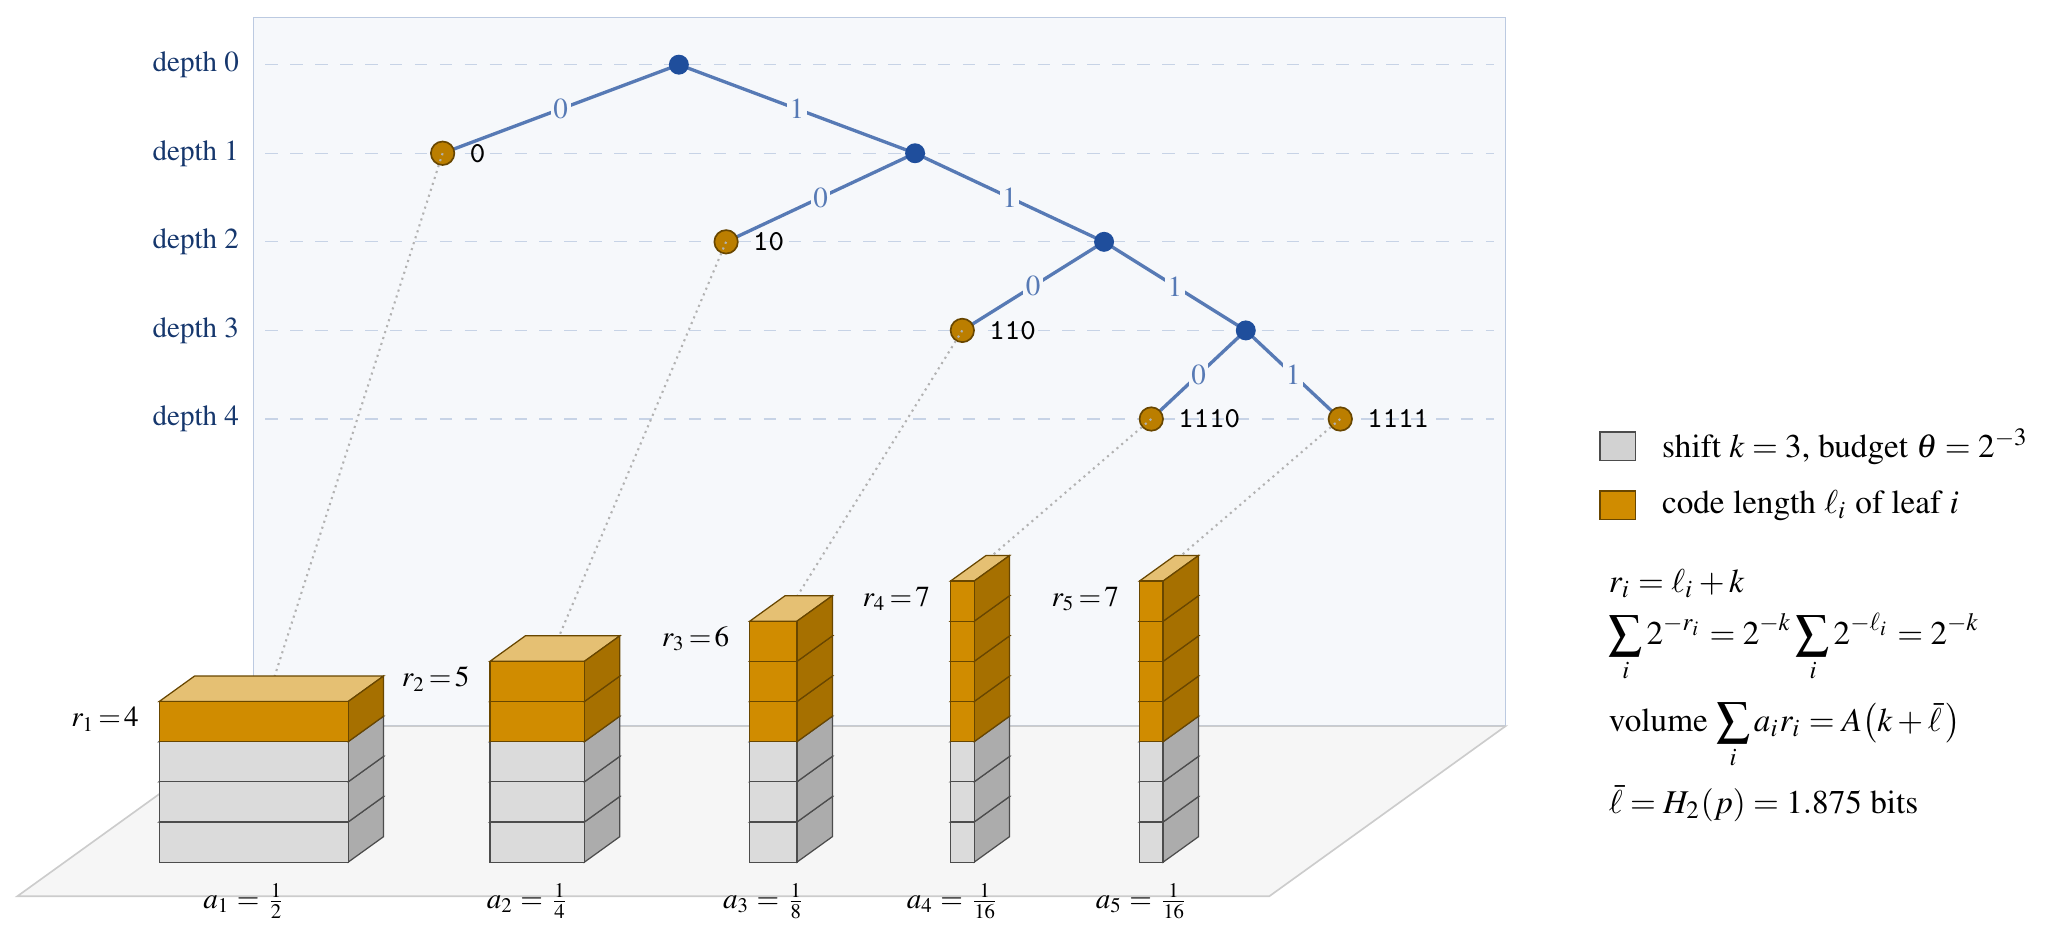
\includegraphics[width=0.92\textwidth]{figures/fig_kraft3d}
\caption{Theorem~\ref{thm:C} for the profile $p=(\frac12,\frac14,\frac18,\frac1{16},\frac1{16})$, $\eps=\frac12$ and $\theta=2^{-3}$. Back wall: the binary Huffman tree, with codewords $0$, $10$, $110$, $1110$, $1111$. Floor: a column for each candidate, of width proportional to its cost $a_{i}$, built from $k=3$ grey blocks, which buy the budget $2^{-3}$, and $\ell_{i}$ gold blocks, one per letter of its codeword. The heights are the optimal numbers of runs $r_{i}=4,5,6,7,7$, the budget is exactly spent, $\sum2^{-r_{i}}=2^{-3}$, and the volume of the columns is the optimal cost $A(k+\bar\ell)$ with $\bar\ell=H_{2}(p)=1.875$.}
\label{fig:kraft}
\end{figure*}

\begin{corollary}\label{cor:huffbounds}
Under the hypotheses of Theorem~\ref{thm:C}, $A(k+H_{D}(p))\le\Vs(D^{-k})<A(k+H_{D}(p)+1)$, with equality on the left if and only if every $p_{i}$ is an integer power of $1/D$.
\end{corollary}

\begin{proof}
Shannon's bounds $H_{D}(p)\le L_{D}(p)<H_{D}(p)+1$ \cite{Sha48,CT06} are the case $\theta=1$ of Theorem~\ref{thm:A}, since $L=\log D$ and $(A/L)H(p)=AH_{D}(p)$; the equality case is that of Proposition~\ref{prop:entropyineq}.
\end{proof}

The strict inequality on the right is slightly better than Theorem~\ref{thm:A}, and Gallager's bound improves it further when the largest cost share is small \cite{Gal78}: the redundancy $L_{2}(p)-H_{2}(p)$ is at most $p_{\max}+0.086$ when the largest share $p_{\max}$ is below one half. So the additive constant $A$ of the entropy law is, in this case, the redundancy of an optimal code.

\subsection{Examples}

Table~\ref{tab:huffman} compares three schedules on two profiles: the Huffman schedule, the ceiling schedule of Theorem~\ref{thm:A}, and the lower bound. On a dyadic profile the three agree. On a profile that is not dyadic the ceiling schedule overspends, because the Shannon lengths $\lceil\log_{2}(1/p_{i})\rceil$ are not optimal, and the Huffman schedule lies between it and the bound.

\begin{table}[b]
\caption{Schedules for $\eps=\frac12$, $\theta=2^{-3}$. Costs are $V/A$.}
\label{tab:huffman}
\centering
\small
\begin{tabular}{@{}l l l@{}}
\toprule
 & $p=(\frac12,\frac14,\frac18,\frac1{16},\frac1{16})$ & $p=(0.4,0.3,0.2,0.1)$ \\
\midrule
Huffman lengths $\ell$ & $(1,2,3,4,4)$ & $(1,2,3,3)$ \\
Huffman schedule $r$ & $(4,5,6,7,7)$ & $(4,5,6,6)$ \\
$\sum2^{-r_{i}}$ & $2^{-3}$ & $2^{-3}$ \\
cost, Huffman & $4.875$ & $4.900$ \\
ceiling schedule $r$ & $(4,5,6,7,7)$ & $(5,5,6,7)$ \\
cost, ceiling & $4.875$ & $5.400$ \\
bound $3+H_{2}(p)$ & $4.875$ & $4.846$ \\
\bottomrule
\end{tabular}
\end{table}

Figure~\ref{fig:huffman} runs the comparison over twelve profiles: uniform, Zipf, geometric and random. The Huffman cost minus $k$ is the Huffman length, which lies in $[H_{2}(p),H_{2}(p)+1)$ and equals $H_{2}(p)$ only for the dyadic profiles.

\begin{figure*}[t]
\centering
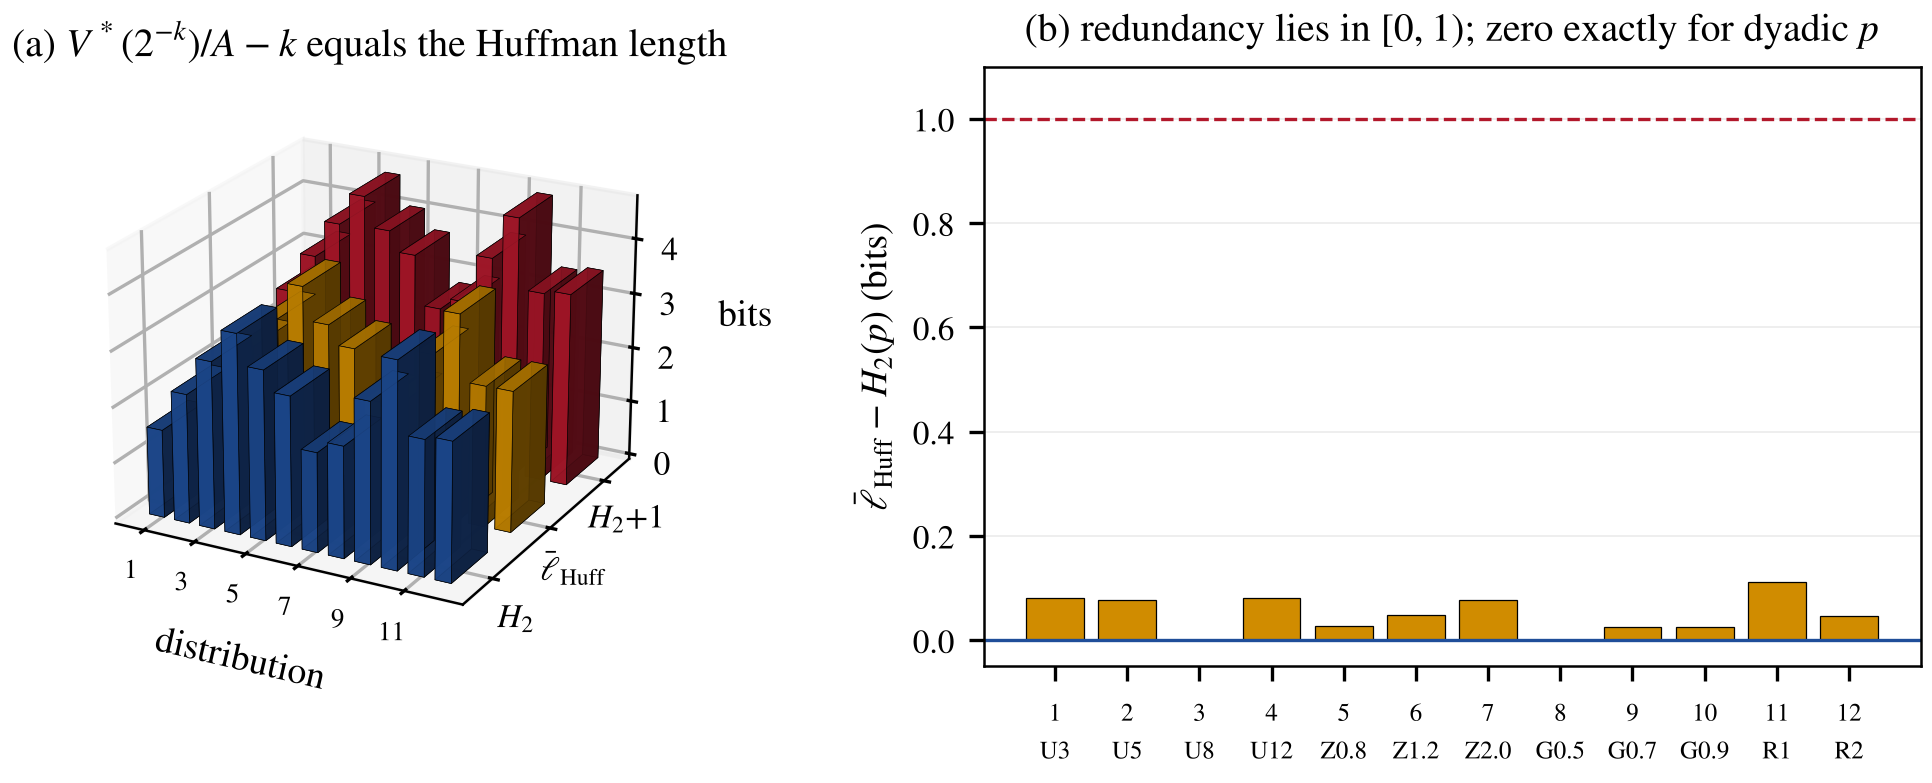
\includegraphics[width=0.98\textwidth]{figures/fig_huffman3d}
\caption{Theorem~\ref{thm:C} on twelve profiles: uniform on $3$, $5$, $8$ and $12$ candidates (U), Zipf with exponents $0.8$, $1.2$ and $2$ on ten (Z), geometric with ratios $0.5$, $0.7$ and $0.9$ on fourteen (G), and two random profiles on nine (R). (a) For each profile, the entropy $H_{2}(p)$, the optimal schedule cost $\Vs(2^{-k})/A-k$, which is the Huffman length, and $H_{2}(p)+1$. (b) The redundancy $\Vs/A-k-H_{2}(p)$, which lies in $[0,1)$; it vanishes on the dyadic profile, the uniform one on eight candidates (green), and is $2.7\times10^{-5}$ for the geometric profile of ratio one half, whose normalised weights differ from powers of two by the factor $2/(2-2^{-13})$. The largest redundancy, $0.112$, is that of the first random profile.}
\label{fig:huffman}
\end{figure*}

\begin{remark}[Larger alphabets]
For $D\ge3$ Huffman's algorithm merges the $D$ smallest weights at each step, after adding zero weights until $n\equiv1\pmod{D-1}$; the dummy candidates receive the longest codewords and cost nothing (Appendix~\ref{app:huffman}). A check of soundness $1/3$ run $r$ times is a ternary codeword of length $r$.
\end{remark}

\section{The R\'enyi law and the duality criterion}\label{sec:renyi}

\subsection{Polynomial checks}

A check is \emph{exponential} when $r$ runs drive its false acceptance probability to $\eps^{r}$, so that the cost of reaching $\delta$ is $a\log(1/\delta)/L$. Many checks are slower. A statistical check that averages $m$ independent samples of a statistic and accepts when the average is close to its target is the basic example.

\begin{example}[Chebyshev checks]\label{ex:chebyshev}
Let a candidate determine a random variable $X$ with variance at most $\sigma^{2}$, with mean $0$ if the candidate is correct and mean at least $2t>0$ if it is incorrect, and let the check accept when the mean of $m$ independent samples is below $t$. By Chebyshev's inequality an incorrect candidate is accepted, and a correct one rejected, with probability at most $\sigma^{2}/(mt^{2})$. So false acceptance probability $\delta$ costs $m=\sigma^{2}/(t^{2}\delta)$ samples: the cost is $a\,\delta^{-1}$ with $a$ proportional to $\sigma^{2}/t^{2}$.
\end{example}

We say a family of checks has \emph{polynomial order} $s>0$ if the check of candidate $i$ reaches false acceptance probability $\delta_{i}\in(0,1]$ at cost $a_{i}\delta_{i}^{-s}$, and that an allocation $\delta$ is $\theta$-sound if $\sum_{i}\delta_{i}\le\theta$. Chebyshev checks have order $1$. Let $\Vs_{s}(\theta)$ be the infimum of $\sum_{i}a_{i}\delta_{i}^{-s}$ over $\theta$-sound allocations. For $0<\alpha<1$ the R\'enyi entropy of order $\alpha$ is
\[
H_{\alpha}(p)=\frac1{1-\alpha}\log\sum_{i}p_{i}^{\alpha},
\]
which decreases from $\log n$ at $\alpha\to0$ to $H(p)$ at $\alpha\to1$ \cite{Ren61,CT06}.

\begin{proof}[Proof of Theorem~\ref{thm:D}]
\emph{Lower bound.} Put $\alpha=1/(1+s)$, so that $1/\alpha=1+s$ and $1/(1-\alpha)=(1+s)/s$ are conjugate exponents. Write $a_{i}^{\alpha}=(a_{i}\delta_{i}^{-s})^{\alpha}\,\delta_{i}^{s\alpha}$ and apply H\"older's inequality:
\[
\begin{aligned}
\sum_{i}a_{i}^{\alpha}&\le\Bigl(\sum_{i}a_{i}\delta_{i}^{-s}\Bigr)^{\alpha}\Bigl(\sum_{i}\delta_{i}^{s\alpha/(1-\alpha)}\Bigr)^{1-\alpha}\\
&=\Bigl(\sum_{i}a_{i}\delta_{i}^{-s}\Bigr)^{\frac1{1+s}}\Bigl(\sum_{i}\delta_{i}\Bigr)^{\frac s{1+s}},
\end{aligned}
\]
since $s\alpha/(1-\alpha)=1$. With $\sum\delta_{i}\le\theta$ and raising to the power $1+s$, $(\sum_{i}a_{i}^{\alpha})^{1+s}\le\theta^{s}\sum_{i}a_{i}\delta_{i}^{-s}$.

\emph{Attainment.} Let $S=\sum_{j}a_{j}^{\alpha}$ and $\delta_{i}=\theta a_{i}^{\alpha}/S$. Then $\sum\delta_{i}=\theta$, $\delta_{i}\le\theta\le1$ because $a_{i}^{\alpha}\le S$, and $\sum_{i}a_{i}\delta_{i}^{-s}=\theta^{-s}S^{s}\sum_{i}a_{i}^{1-s\alpha}=\theta^{-s}S^{s}\sum_{i}a_{i}^{\alpha}=\theta^{-s}S^{1+s}$, because $1-s\alpha=\alpha$.

\emph{Entropy form.} $S=A^{\alpha}\sum_{i}p_{i}^{\alpha}$, so $S^{1+s}=A\,(\sum_{i}p_{i}^{\alpha})^{1+s}$, and $(1+s)\log\sum p_{i}^{\alpha}=\frac{1+s}{s}\,s\log\sum p_{i}^{\alpha}=s\,H_{\alpha}(p)$, since $1-\alpha=s/(1+s)$.

\emph{The limit $s\to0$.} For finitely many candidates $\alpha\mapsto\log\sum p_{i}^{\alpha}$ is smooth and vanishes at $\alpha=1$ with derivative $\sum p_{i}\log p_{i}=-H(p)$ there, so $H_{\alpha}(p)=H(p)+O(1-\alpha)=H(p)+O(s)$. Hence $\Vs_{s}(\theta)/A=\exp\bigl(s(H_{\alpha}(p)+\log\frac1\theta)\bigr)=1+s\bigl(H(p)+\log\frac1\theta\bigr)+O(s^{2})$.
\end{proof}

The optimal allocation gives the $i$-th check the share $a_{i}^{\alpha}/S$ of the budget, a flattened version of the share $a_{i}/A$ of the exponential case: when checks are slow, expensive checks must still be made quite reliable, because buying reliability anywhere is costly. The two laws are related by a limit. Since $\frac1L\log\frac1\delta=\lim_{s\to0}\frac{\delta^{-s}-1}{sL}$, the cost of an exponential check is the derivative at $s=0$ of the cost of a polynomial one, and
\[
\lim_{s\to0}\frac{\Vs_{s}(\theta)-A}{sL}=\frac AL\Bigl(H(p)+\log\frac1\theta\Bigr),
\]
which is the real relaxation of the entropy law (Proposition~\ref{prop:shape}). Campbell's coding theorem has the same structure, with exponentially weighted codeword lengths and the R\'enyi entropy of order $1/(1+t)$ \cite{Cam65}.

\begin{corollary}[Equal costs]\label{cor:polyuniform}
For $n$ candidates of cost $a$ and checks of order $s$, $\Vs_{s}(\theta)=a\,n^{1+s}\theta^{-s}$. Chebyshev checks cost $an^{2}/\theta$, against $(an/L)\log(n/\theta)+O(an)$ for exponential checks.
\end{corollary}

So the tax per candidate is $(n/\theta)^{s}$ for polynomial checks and $\log(n/\theta)/L$ for exponential ones: a statistical check that is not amplified exponentially makes the certification of a long run of modifications quadratically expensive. Figure~\ref{fig:renyi} shows the law and its tangent at $s=0$.

\begin{figure*}[t]
\centering
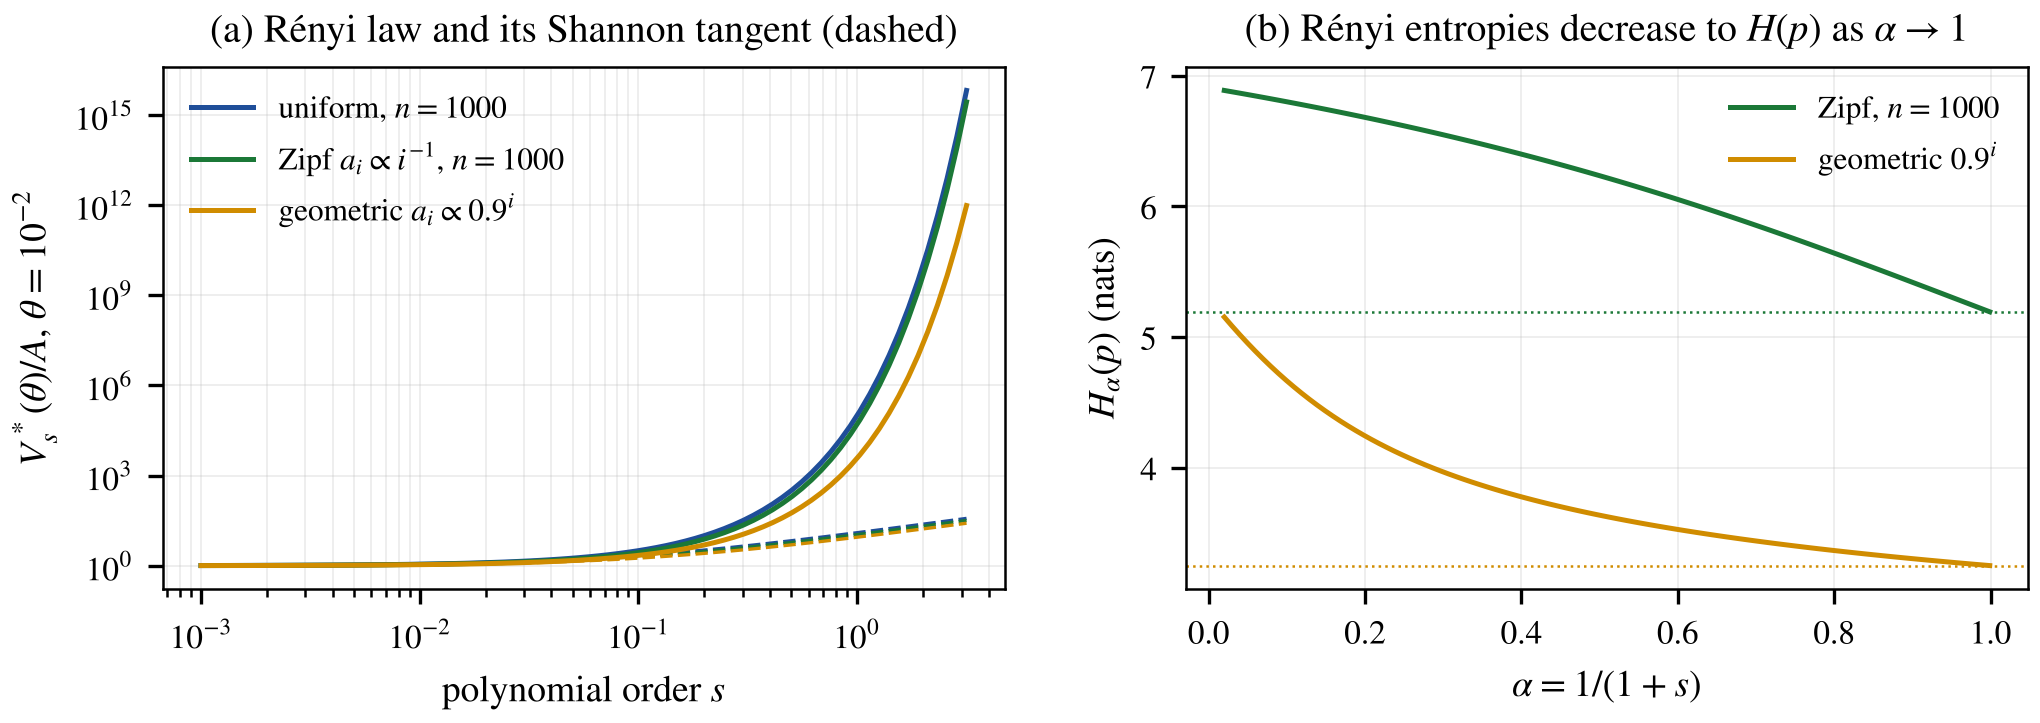
\includegraphics[width=0.98\textwidth]{figures/fig_renyi}
\caption{The R\'enyi law, Theorem~\ref{thm:D}. (a) $\Vs_{s}(\theta)/A=\theta^{-s}e^{sH_{1/(1+s)}(p)}$ at $\theta=10^{-2}$ for a uniform profile and a Zipf profile on a thousand candidates and a geometric profile of ratio $0.9$, with the Shannon tangents $1+s(H(p)+\log\frac1\theta)$ (dashed). The tangents are exact as $s\to0$ and the flat profile is the most expensive at every order. (b) The R\'enyi entropies $H_{\alpha}(p)$ of the Zipf and geometric profiles as functions of $\alpha=1/(1+s)$, decreasing to the Shannon entropy (dotted) as $\alpha\to1$.}
\label{fig:renyi}
\end{figure*}

\subsection{The duality criterion}

For infinitely many candidates the question is not the value of the optimum but whether a sound allocation of finite cost exists. The answer, for every cost function, is a single series.

Let $\kappa\colon(0,1]\to[0,\infty)$ be the cost, per unit of $a$, of making a check accept an incorrect candidate with probability at most $\delta$; so $\kappa(\delta)=\log(1/\delta)/L$ for exponential checks with a real number of runs and $\kappa(\delta)=\delta^{-s}$ for checks of order $s$. Define the \emph{dual cost}
\[
\psi(u)=\inf_{0<\delta\le1}\bigl(\kappa(\delta)+u\delta\bigr),\qquad u\ge0,
\]
the least cost of a check when each unit of false acceptance probability is charged $u$. It is the concave conjugate of $\kappa$ restricted to $(0,1]$.

\begin{theorem}[Duality criterion]\label{thm:dual}
Let $a_{n}>0$. The following are equivalent.
\begin{enumerate}[label=\textup{(\alph*)},leftmargin=2.2em,itemsep=1pt]
\item There are $\delta_{n}\in(0,1]$ with $\sum_{n}\delta_{n}<\infty$ and $\sum_{n}a_{n}\kappa(\delta_{n})<\infty$.
\item $\sum_{n}a_{n}\psi(\lambda/a_{n})<\infty$ for some $\lambda>0$.
\item $\sum_{n}a_{n}\psi(\lambda/a_{n})<\infty$ for every $\lambda>0$.
\end{enumerate}
When they hold, for every $\theta>0$ there are $\delta_{n}\in(0,1]$ with $\sum\delta_{n}\le\theta$ and $\sum a_{n}\kappa(\delta_{n})<\infty$.
\end{theorem}

\begin{proof}
(a)$\Rightarrow$(c). For every $\lambda>0$ and $n$, $0\le a_{n}\psi(\lambda/a_{n})\le a_{n}\kappa(\delta_{n})+\lambda\delta_{n}$, and the right side is summable.
(c)$\Rightarrow$(b) is trivial.
(b)$\Rightarrow$(a). By the definition of the infimum choose $\delta_{n}\in(0,1]$ with $\kappa(\delta_{n})+(\lambda/a_{n})\delta_{n}\le\psi(\lambda/a_{n})+2^{-n}/a_{n}$. Then $a_{n}\kappa(\delta_{n})+\lambda\delta_{n}\le a_{n}\psi(\lambda/a_{n})+2^{-n}$, a summable bound for two nonnegative terms, so both $\sum a_{n}\kappa(\delta_{n})$ and $\sum\delta_{n}$ converge.
For the last claim choose $N$ with $\sum_{n>N}\delta_{n}\le\theta/2$ and replace $\delta_{n}$ by $\theta/(2N)$ for $n\le N$; this changes finitely many finite terms of the cost.
\end{proof}

\begin{proposition}[The two dual costs]\label{prop:dualcosts}
\begin{enumerate}[label=\textup{(\roman*)},leftmargin=2.2em,itemsep=1pt]
\item For exponential checks, $\kappa(\delta)=\log(1/\delta)/L$, the dual is
\[
\psi(u)=\begin{cases}(1+\log(uL))/L,&uL\ge1,\\ u,&uL<1.\end{cases}
\]
\item For checks of order $s$, $\kappa(\delta)=\delta^{-s}$, the dual is
\[
\psi(u)=\begin{cases}(1+s)\,s^{-s/(1+s)}u^{s/(1+s)},&u\ge s,\\ 1+u,&u<s.\end{cases}
\]
\end{enumerate}
\end{proposition}

\begin{proof}
Both functions $\delta\mapsto\kappa(\delta)+u\delta$ are convex on $(0,1]$. In (i) the derivative $-1/(L\delta)+u$ vanishes at $\delta=1/(uL)$, which lies in $(0,1]$ exactly when $uL\ge1$, with value $\log(uL)/L+1/L$; otherwise the derivative is negative on $(0,1]$ and the minimum is at $\delta=1$. In (ii) the derivative $-s\delta^{-s-1}+u$ vanishes at $\delta=(s/u)^{1/(1+s)}$, which lies in $(0,1]$ exactly when $u\ge s$, with value $(s/u)^{-s/(1+s)}+u(s/u)^{1/(1+s)}=(1+s)s^{-s/(1+s)}u^{s/(1+s)}$; otherwise the minimum is at $\delta=1$.
\end{proof}

\begin{corollary}\label{cor:dualcases}
Let $a_{n}\to0$.
\begin{enumerate}[label=\textup{(\roman*)},leftmargin=2.2em,itemsep=1pt]
\item Exponential checks with real numbers of runs admit a sound allocation of finite cost if and only if $\sum a_{n}<\infty$ and $\sum a_{n}\log(1/a_{n})<\infty$.
\item Checks of order $s$ admit one if and only if $\sum a_{n}^{1/(1+s)}<\infty$.
\end{enumerate}
\end{corollary}

\begin{proof}
For large $n$, $u=\lambda/a_{n}$ is large, and by Proposition~\ref{prop:dualcosts} $a_{n}\psi(\lambda/a_{n})$ equals $\frac{a_{n}}L\bigl(1+\log(\lambda L)+\log\frac1{a_{n}}\bigr)$ in case (i) and a constant multiple of $a_{n}^{1/(1+s)}$ in case (ii). In case (i) the sum converges if and only if $\sum a_{n}(1+\log\frac1{a_{n}})$ does, and both terms are eventually positive. Theorem~\ref{thm:dual} concludes.
\end{proof}

The integer version needs no duality.

\begin{proposition}[Integer schedules]\label{prop:integer}
Let $0<a_{n}\le1$ with $\sum a_{n}<\infty$. There is $r\in\NN^{\NN}$ with $\sum\eps^{r_{n}}<\infty$ and $\sum a_{n}r_{n}<\infty$ if and only if $\sum a_{n}\log(1/a_{n})<\infty$; the schedule $r_{n}=\lceil\log(1/a_{n})/L\rceil$ then works, and adding $k$ runs to every check multiplies $\sum\eps^{r_{n}}$ by $\eps^{k}$.
\end{proposition}

\begin{proof}
If $r$ is such a schedule, Lemma~\ref{lem:gibbs} with $x=a_{n}$ and $y=\eps^{r_{n}}$ gives $a_{n}\log(1/a_{n})\le a_{n}r_{n}L+\eps^{r_{n}}-a_{n}\le L\,a_{n}r_{n}+\eps^{r_{n}}$, a summable bound for a nonnegative sequence. Conversely $r_{n}=\lceil\log(1/a_{n})/L\rceil$ gives $\eps^{r_{n}}\le a_{n}$ and $a_{n}r_{n}\le a_{n}\log(1/a_{n})/L+a_{n}$. The last claim is $\eps^{r_{n}+k}=\eps^{k}\eps^{r_{n}}$.
\end{proof}

Theorem~\ref{thm:dual} is the infinite form of the entropy and R\'enyi laws: it says which cost profiles can be certified at all, and Section~\ref{sec:singularity} applies it to self-improving chains.

\section{Self-improvement chains}\label{sec:chains}

\subsection{The chain}

A BLLM improves itself in steps. At step $i$ the generator proposes candidates for the $i$-th modification until one is kept, then moves to step $i+1$. A candidate for step $i$ costs $g_{i}\ge0$ to generate, is incorrect with probability $\rho_{i}$, independently of everything else, and is checked by $r_{i}$ runs of a sharp check of soundness $\eps$ and cost $a_{i}$ per run, stopping at the first rejection. Let $T_{i}$ be the total cost of step $i$, $F$ the number of steps whose kept candidate is incorrect, $G=\sum g_{i}$, and write $\beta_{i}=\eps^{r_{i}}$.

\begin{lemma}[One step]\label{lem:onestep}
Let $s_{i}=1-\rho_{i}+\rho_{i}\beta_{i}$ be the probability that a candidate is kept and $\pi_{i}=\rho_{i}\beta_{i}/s_{i}$ the probability that the kept candidate is incorrect. Then
\[
g_{i}+a_{i}r_{i}\ \le\ \EE\,T_{i}\ \le\ \frac{g_{i}+a_{i}r_{i}}{1-\rho_{i}},\qquad \rho_{i}\beta_{i}\ \le\ \pi_{i}\ \le\ \frac{\rho_{i}\beta_{i}}{1-\rho_{i}} .
\]
\end{lemma}

\begin{proof}
The number of candidates proposed at step $i$ is geometric with success probability $s_{i}$, so its mean is $1/s_{i}$, and by Wald's identity $\EE\,T_{i}$ is $1/s_{i}$ times the expected cost $c_{i}$ of one candidate. A candidate costs $g_{i}$ plus at most $r_{i}$ runs, so $c_{i}\le g_{i}+a_{i}r_{i}$, and $s_{i}\ge1-\rho_{i}$; this is the upper bound. The kept candidate passed all its $r_{i}$ runs, so it alone costs $g_{i}+a_{i}r_{i}$; this is the lower bound. The bounds on $\pi_{i}$ follow from $1-\rho_{i}\le s_{i}\le1$.
\end{proof}

\begin{mainthm}[Chain law]\label{thm:B}
Let $0<\rho_{\ast}\le\rho_{i}\le\bar\rho<1$ for every $i$, and let $C^{*}(\theta)$ be the least value of $\sum_{i}\EE\,T_{i}$ over schedules with $\EE F\le\theta$. Then
\[
\begin{aligned}
C^{*}(\theta)&\ \ge\ G+\frac AL\Bigl(H(p)+\log\frac{\rho_{\ast}}{\theta}\Bigr),\\
C^{*}(\theta)&\ \le\ \frac1{1-\bar\rho}\Bigl[G+\frac AL\Bigl(H(p)+\log\frac{\bar\rho}{(1-\bar\rho)\theta}\Bigr)+A\Bigr],
\end{aligned}
\]
the upper bound for $0<\theta\le\bar\rho/(1-\bar\rho)$.
\end{mainthm}

\begin{proof}
$\EE F=\sum_{i}\pi_{i}$. If $\EE F\le\theta$, then $\rho_{\ast}\sum\beta_{i}\le\sum\pi_{i}\le\theta$ by Lemma~\ref{lem:onestep}, so $r$ is feasible for the budget $\theta/\rho_{\ast}$, and Proposition~\ref{prop:entropyineq} gives $V(r)\ge(A/L)(H+\log(\rho_{\ast}/\theta))$; also $\sum\EE\,T_{i}\ge G+V(r)$. Conversely let $\theta'=\theta(1-\bar\rho)/\bar\rho\le1$ and let $r$ be the ceiling schedule for $\theta'$. Then $\EE F\le\frac{\bar\rho}{1-\bar\rho}\sum\beta_{i}\le\theta$, and $\sum\EE\,T_{i}\le(G+V(r))/(1-\bar\rho)$ with $V(r)\le(A/L)(H+\log\frac1{\theta'})+A$ by Theorem~\ref{thm:A}.
\end{proof}

So the cost of a sound chain is the entropy law with the budget rescaled by the error rate of the generator, plus the cost of generation, inflated at most by the factor $1/(1-\bar\rho)$ for the retries. A better generator, one with smaller $\bar\rho$, moves the two bounds together.

\subsection{Checking steps or checking outcomes}

A chain of $n$ steps can be checked step by step, or run to the end and checked once. Process supervision and outcome supervision are the two names of this choice for language models \cite{UKK22,LKB23}, and the following theorem compares their costs when the checks are given.

Consider $n$ steps, each correct with probability $1-\rho_{i}$, each costing one unit to generate. \emph{Step gating} checks step $i$ with a check that accepts a correct step with probability $1-\eta$ and an incorrect one with probability $\delta$, and regenerates the step until it is accepted. \emph{Outcome gating} generates all $n$ steps, checks the outcome with a check that accepts a correct chain with probability $1-\eta_{o}$ and an incorrect one with probability $\delta_{o}$, and regenerates the whole chain until it is accepted. A chain is correct when all its steps are. The \emph{precision} of a protocol is the probability that the chain it returns is correct.

\begin{theorem}[Step and outcome gating]\label{thm:gating}
Let $c=\prod_{i}(1-\rho_{i})$ and $x_{i}=\rho_{i}\delta/((1-\rho_{i})(1-\eta))$.
\begin{enumerate}[label=\textup{(\roman*)},leftmargin=2.2em,itemsep=1pt]
\item Step gating has expected cost $\sum_{i}1/s_{i}$ with $s_{i}=(1-\rho_{i})(1-\eta)+\rho_{i}\delta$, and precision $\prod_{i}(1+x_{i})^{-1}$, which lies between $e^{-\sum x_{i}}$ and $e^{-\sum x_{i}/(1+x_{i})}$.
\item Outcome gating has expected cost $n/s_{o}$ with $s_{o}=c(1-\eta_{o})+(1-c)\delta_{o}$, and precision $\bigl(1+(1-c)\delta_{o}/(c(1-\eta_{o}))\bigr)^{-1}$.
\item With perfect checks and $\rho_{i}=\rho$, the ratio of the expected cost of outcome gating to that of step gating is $(1-\rho)^{-(n-1)}\ge\max\bigl(1+(n-1)\rho,\ e^{(n-1)\rho}\bigr)$.
\item Let $\rho_{i}=\rho$, $0<\zeta<1$ and $\ell=\log\frac1{1-\zeta}$. Step gating reaches precision $1-\zeta$ if $\delta\le(1-\rho)(1-\eta)\ell/(\rho n)$, and only if $\delta\le(1-\rho)(1-\eta)\ell/(\rho(n-\ell))$ when $n>\ell$. Outcome gating reaches precision $1-\zeta$ if and only if
\[
\delta_{o}\le\frac{\zeta}{1-\zeta}\cdot\frac{c(1-\eta_{o})}{1-c},\qquad c=(1-\rho)^{n}.
\]
\end{enumerate}
\end{theorem}

\begin{proof}
(i) Step $i$ is accepted at each attempt with probability $s_{i}$, so it takes $1/s_{i}$ attempts on average, and the accepted step is correct with probability $(1-\rho_{i})(1-\eta)/s_{i}=1/(1+x_{i})$. The steps are independent, so the precision is the product. For $x\ge0$, $x/(1+x)\le\log(1+x)\le x$, which gives the two exponential bounds.
(ii) The same argument with one step of cost $n$, acceptance probability $s_{o}$ and probability $c(1-\eta_{o})/s_{o}$ that the accepted chain is correct.
(iii) With $\eta=\delta=0$ step gating costs $n/(1-\rho)$ and outcome gating $n/(1-\rho)^{n}$. Bernoulli's inequality gives $(1+\rho)^{n-1}\ge1+(n-1)\rho$, and $(1-\rho)^{-1}\ge1+\rho$, so $(1-\rho)^{-(n-1)}\ge1+(n-1)\rho$; and $1-\rho\le e^{-\rho}$ gives the exponential bound.
(iv) By (i) the precision is $(1+x)^{-n}$ with $x=\rho\delta/((1-\rho)(1-\eta))$, and it is at least $1-\zeta$ exactly when $n\log(1+x)\le\ell$. If $x\le\ell/n$ this holds because $\log(1+x)\le x$. If it holds, then $nx/(1+x)\le\ell$, that is $x\le\ell/(n-\ell)$. For outcome gating, (ii) gives precision at least $1-\zeta$ exactly when $(1-c)\delta_{o}/(c(1-\eta_{o}))\le\zeta/(1-\zeta)$.
\end{proof}

The theorem separates the two protocols by an exponential. A step check needs false acceptance rate of order $1/n$, which an exponential check reaches with $\log n/L$ runs, so step gating with exponential checks costs order $n\log n$, as Corollary~\ref{cor:uniform} predicts. An outcome check needs false acceptance rate of order $\zeta(1-\rho)^{n}$, which costs $n\log\frac1{1-\rho}/L$ runs on every attempt, and even a perfect outcome check leaves the factor $(1-\rho)^{-(n-1)}$ of retries. Figure~\ref{fig:gating} draws both effects, and Fig.~\ref{fig:gatingflow} the two protocols.

\begin{figure*}[t]
\centering
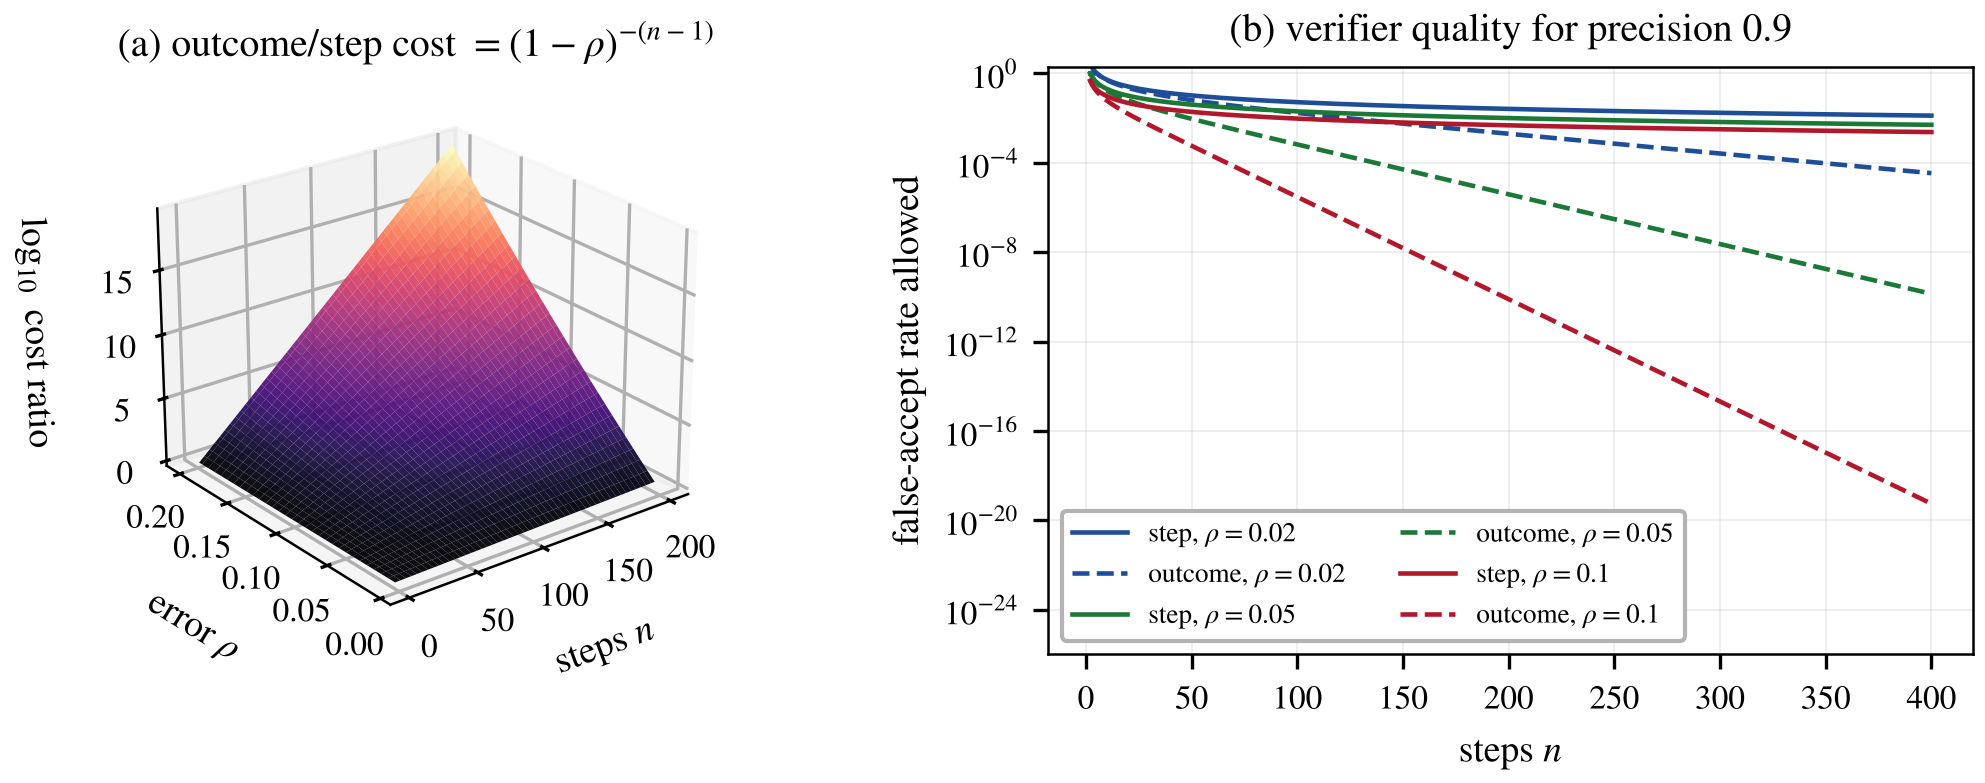
\includegraphics[width=0.98\textwidth]{figures/fig_gating}
\caption{Theorem~\ref{thm:gating}. (a) The ratio $(1-\rho)^{-(n-1)}$ of the expected costs of outcome and step gating with perfect checks, on a logarithmic scale, for up to two hundred steps and error rates $\rho\le0.2$. (b) The false acceptance rate a check may have to reach precision $0.9$ with $\eta=0$: for step gating (solid lines and shaded bands between the sufficient and the necessary rate of part (iv)) it decreases like $1/n$, for outcome gating (dashed) like $(1-\rho)^{n}$.}
\label{fig:gating}
\end{figure*}

\begin{figure*}[t]
\centering
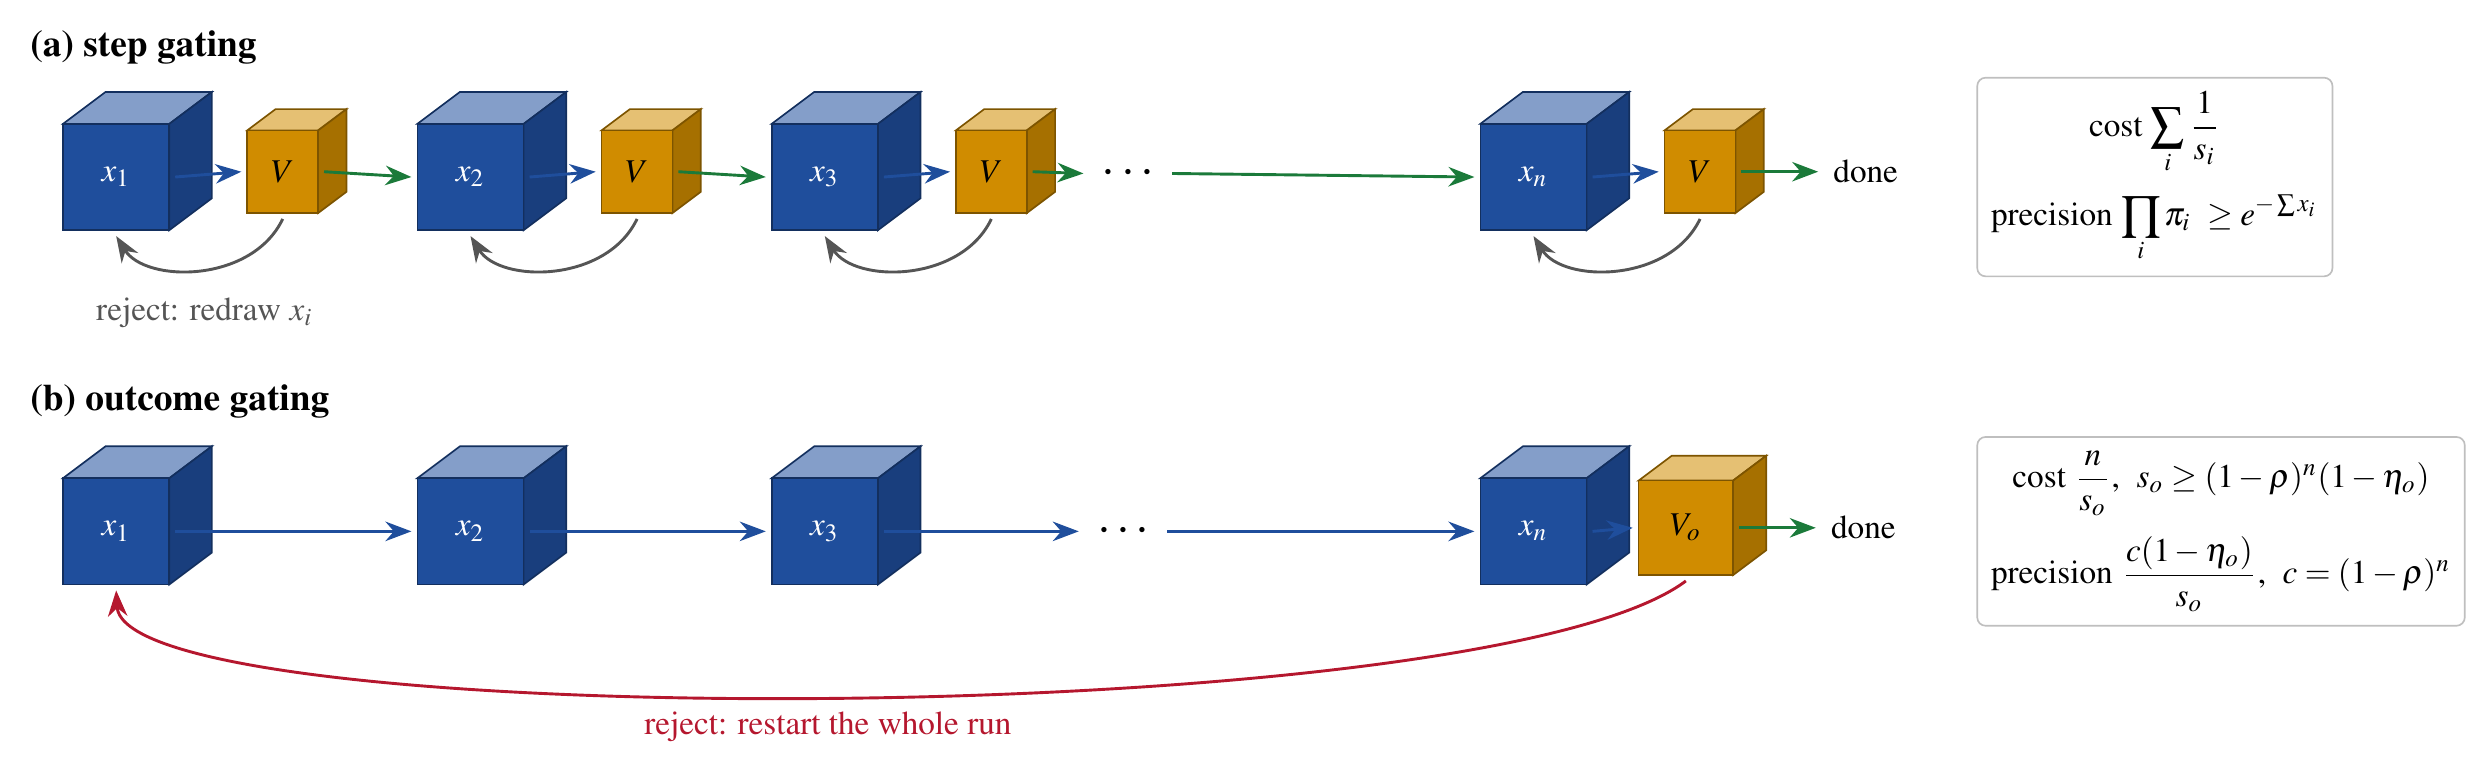
\includegraphics[width=0.94\textwidth]{figures/fig_gatingflow}
\caption{The two protocols of Theorem~\ref{thm:gating}. (a) Step gating: each step is generated and checked, and regenerated until accepted; the cost is $\sum1/s_{i}$ and the precision $\prod\pi_{i}\ge e^{-\sum x_{i}}$. (b) Outcome gating: the chain is generated to the end and checked once, and regenerated until accepted; the acceptance probability is at least $(1-\rho)^{n}(1-\eta_{o})$, the cost is $n/s_{o}$ and the precision $c(1-\eta_{o})/s_{o}$.}
\label{fig:gatingflow}
\end{figure*}

\begin{remark}[Relation to learning from outcomes]
Jia, Rakhlin and Xie proved that learning a policy from outcome rewards is statistically no harder than learning it from step rewards, up to polynomial factors in the horizon \cite{JRX25}. Theorem~\ref{thm:gating} is about a different cost, that of certifying a chain with checks that are already given, and the two results are compatible: a learner may extract as much from outcomes as from steps, while a certifier that sees only outcomes pays exponentially in retries and in the reliability its check must have. Rohatgi and coauthors observe the same amplification of verifier error along a generation from the side of sampling \cite{RSS25}.
\end{remark}

\section{Sound singularities}\label{sec:singularity}

\subsection{Singular chains}

Let the chain of Section~\ref{sec:chains} run forever: step $n\ge1$ costs $g_{n}$ per candidate to generate and $a_{n}$ per run to check, is incorrect with probability $\rho_{n}$, and is checked by $r_{n}$ runs of a sharp check of soundness $\eps$, all steps independent. The total cost is $T_{\infty}=\sum_{n}T_{n}$ and $F$ counts the steps whose kept candidate is incorrect.

\begin{definition}\label{def:singular}
The chain is \emph{singular} if $\EE\,T_{\infty}<\infty$, and \emph{sound} if $F<\infty$ almost surely.
\end{definition}

If cost is time, a singular chain completes infinitely many improvements in finite expected time, which is the vertical asymptote of the explosion literature \cite{Goo66,Ord26}; if cost is compute or energy, it completes them on a finite budget. Soundness asks that only finitely many of the improvements be wrong, so that from some step on the system is correct.

\begin{proof}[Proof of Theorem~\ref{thm:E}]
Put $\gamma=1-\bar\rho$. By Lemma~\ref{lem:onestep}, $g_{n}+a_{n}r_{n}\le\EE\,T_{n}\le(g_{n}+a_{n}r_{n})/\gamma$ and $\rho_{\ast}\eps^{r_{n}}\le\pi_{n}\le\eps^{r_{n}}/\gamma$. So $\EE\,T_{\infty}<\infty$ if and only if $\sum(g_{n}+a_{n}r_{n})<\infty$, and $\sum\pi_{n}<\infty$ if and only if $\sum\eps^{r_{n}}<\infty$.

(i) Let $E_{n}$ be the event that the candidate kept at step $n$ is incorrect, so $F=\sum\ind_{E_{n}}$ and the $E_{n}$ are independent with $\PR(E_{n})=\pi_{n}<1$. If $\sum\pi_{n}<\infty$, then $\EE F<\infty$, so $F<\infty$ almost surely (this is the first Borel--Cantelli lemma \cite{Bor09,Dur19}), and $\PR(F=0)=\prod_{n}(1-\pi_{n})>0$, because a product of factors in $(0,1]$ converges to a positive limit when the sum of the complements converges. If $\sum\pi_{n}=\infty$, the second Borel--Cantelli lemma for independent events gives $\PR(E_{n}\text{ infinitely often})=1$, so $F=\infty$ almost surely and $\PR(F=0)=0$.

(ii) If every $r_{n}\ge1$, then $\sum a_{n}r_{n}\ge\sum a_{n}$, so a singular chain needs $\sum g_{n}<\infty$ and $\sum a_{n}<\infty$; conversely $r_{n}=1$ gives $\EE\,T_{\infty}\le\sum(g_{n}+a_{n})/\gamma<\infty$.

(iii) A sound singular chain needs $\sum g_{n}<\infty$, $\sum a_{n}r_{n}<\infty$ and $\sum\eps^{r_{n}}<\infty$. The last forces $r_{n}\ge1$ for all large $n$, so $\sum a_{n}<\infty$, and Proposition~\ref{prop:integer} (applied to the tail on which $a_{n}\le1$) gives $\sum a_{n}\log(1/a_{n})<\infty$. Conversely, under the three conditions, the schedule $r_{n}=\lceil\log(1/a_{n})/L\rceil$ of Proposition~\ref{prop:integer}, raised to at least one run, has $\sum a_{n}r_{n}<\infty$ and $\sum\eps^{r_{n}}<\infty$.
\end{proof}

The theorem has a simple form: the chain can reach the asymptote if the steps get cheap fast enough, and it can reach it soundly if they get cheap fast enough to pay for the entropy. Since $a\log(1/a)\ge a$ for $a\le1/e$, the second condition is strictly stronger, and the next corollary shows that the gap between them is not empty.

\begin{corollary}[The soundness gap]\label{cor:gap}
Let $a_{n}=1/(n\log^{\beta}n)$ for $n\ge3$, with $\sum g_{n}<\infty$. A singular chain with every step checked exists if and only if $\beta>1$, and a sound singular chain exists if and only if $\beta>2$. For $1<\beta\le2$ every singular chain keeps infinitely many incorrect modifications almost surely.
\end{corollary}

\begin{proof}
The series $\sum1/(n\log^{c}n)$ converges if and only if $c>1$, by Cauchy's condensation test: its terms decrease, and $2^{k}$ times the term at $n=2^{k}$ is $(k\log2)^{-c}$ (Appendix~\ref{app:condensation}). So $\sum a_{n}<\infty$ if and only if $\beta>1$. For the entropy, $\log(1/a_{n})=\log n+\beta\log\log n$, which lies between $\log n$ and $2\log n$ for all large $n$, so $a_{n}\log(1/a_{n})$ lies between $1/(n\log^{\beta-1}n)$ and twice it, and $\sum a_{n}\log(1/a_{n})<\infty$ if and only if $\beta-1>1$. Theorem~\ref{thm:E} concludes; the last claim is part (i), since a singular chain with $1<\beta\le2$ cannot have $\sum\eps^{r_{n}}<\infty$.
\end{proof}

Figure~\ref{fig:price}(b) shows the condensed partial sums of the two series for three values of $\beta$.

\subsection{Power laws}

The case that matters for growth models is a power law, $a_{n}=n^{-p}$ with $p>1$. Then $A=\zeta(p)$, the profile has entropy
\[
H(p)=\log\zeta(p)+p\,\frac{-\zeta'(p)}{\zeta(p)},
\]
by \eqref{eq:AH}, and $\sum a_{n}\log(1/a_{n})=p\sum n^{-p}\log n<\infty$ for every $p>1$. So every power law admits a sound singularity, and the question is its price.

\begin{proposition}[Price of a power-law takeoff]\label{prop:powerlaw}
As $p\to1^{+}$,
\[
\begin{aligned}
H(p)&=\frac1{p-1}+\log\frac1{p-1}+O(1),\\
\frac{\Vs(\theta)}{A}&=\frac1{(p-1)L}+O\Bigl(\log\frac1{p-1}\Bigr),
\end{aligned}
\]
for fixed $\theta\in(0,1]$ and $\eps$, so that $\Vs(\theta)=\frac{1}{(p-1)^{2}L}\bigl(1+O((p-1)\log\frac1{p-1})\bigr)$.
\end{proposition}

\begin{proof}
Put $t=p-1$. Comparing the decreasing function $x^{-p}$ with its integral, $1/t=\int_{1}^{\infty}x^{-p}\,dx\le\zeta(p)\le1+1/t$. The function $f(x)=x^{-p}\log x$ vanishes at $1$, increases on $[1,e^{1/p}]$ and decreases afterwards, with maximum $1/(pe)$, so $\bigl|\sum_{n\ge1}f(n)-\int_{1}^{\infty}f\bigr|\le1/(pe)$ (Appendix~\ref{app:zeta}); and $\int_{1}^{\infty}x^{-p}\log x\,dx=1/t^{2}$. Hence $-\zeta'(p)=1/t^{2}+O(1)$ and
\[
\frac{-p\zeta'(p)}{\zeta(p)}=\frac{(1+t)(t^{-2}+O(1))}{t^{-1}(1+O(t))}=\frac1t+O(1)
\]
and $\log\zeta(p)=\log\frac1t+O(t)$.
This is the first formula. The second follows from Theorem~\ref{thm:A}, Proposition~\ref{prop:infinite} and $A=1/t+O(1)$.
\end{proof}

The constant term is $1-\gamma_{E}$, where $\gamma_{E}$ is Euler's constant, as the Laurent expansion $\zeta(p)=1/t+\gamma_{E}+O(t)$ shows; at $p=1.1$ the three terms give $12.725$ against the exact $H=12.745$. So the cheapest sound takeoff along a power law near the critical exponent costs, per unit of the cost of one run per step, about $1/((p-1)L)$, and in total about $1/((p-1)^{2}L)$: the soundness of the takeoff is paid for with one extra factor $1/(p-1)$ (Fig.~\ref{fig:price}(a)).

\begin{figure*}[t]
\centering
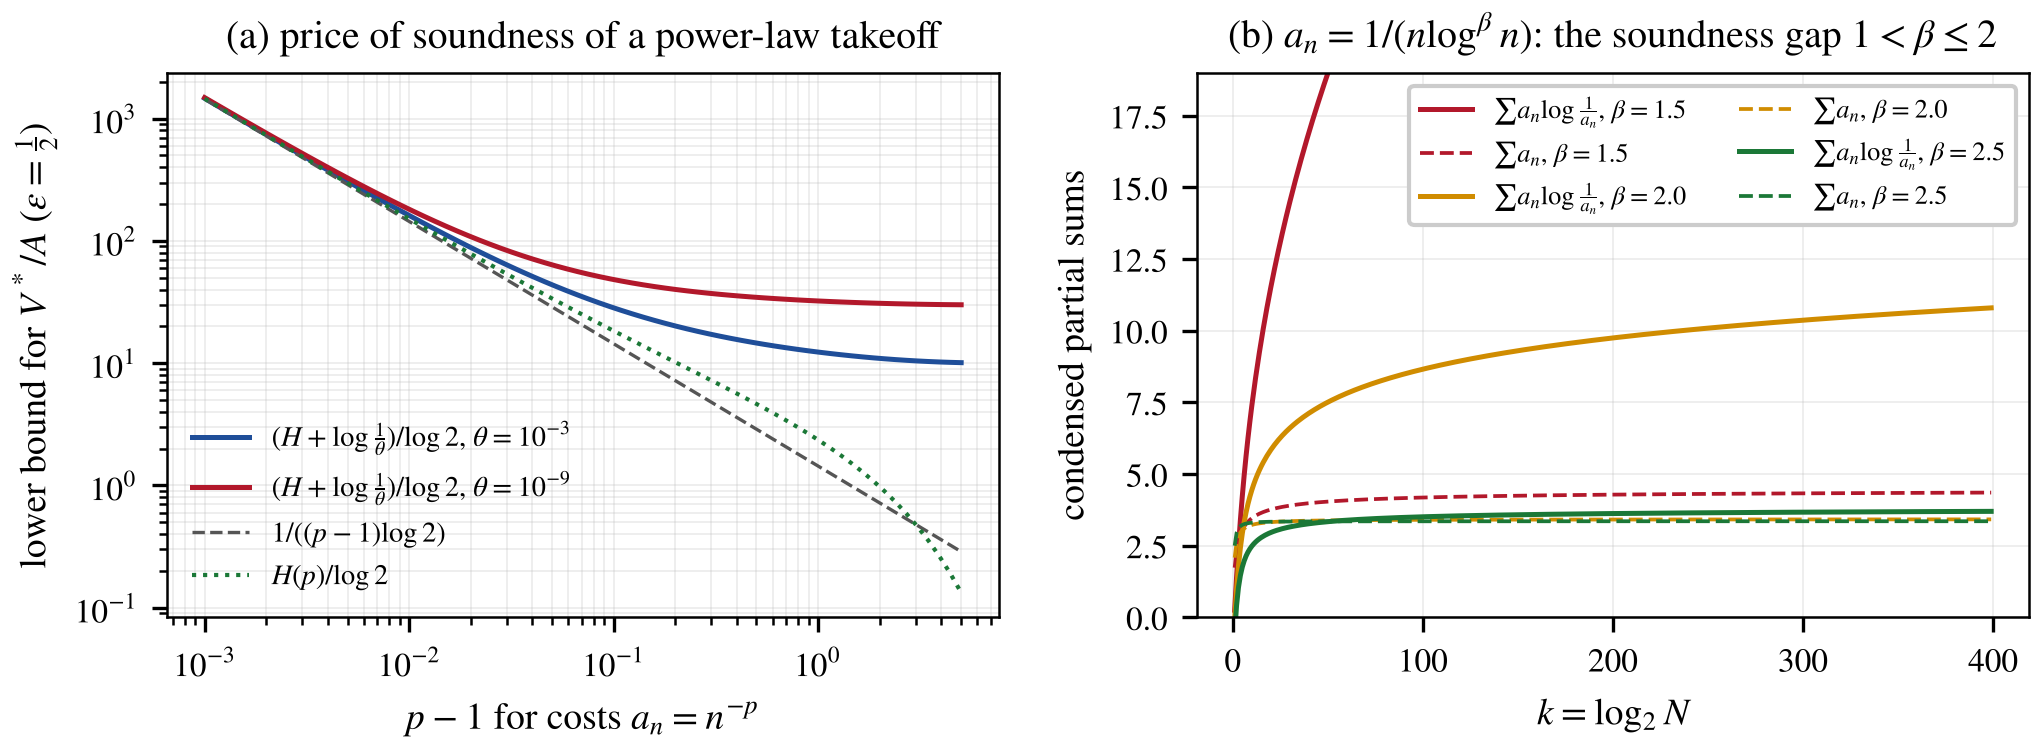
\includegraphics[width=0.98\textwidth]{figures/fig_price}
\caption{(a) The lower bound $(H(p)+\log\frac1\theta)/\log2$ for $\Vs/A$ along the power laws $a_{n}=n^{-p}$, with $\eps=\frac12$ and $\theta=10^{-3}$, $10^{-9}$; as $p\to1$ it approaches $1/((p-1)\log2)$ (dashed), the term that dominates the entropy (dotted). (b) The soundness gap of Corollary~\ref{cor:gap}: condensed partial sums of $\sum a_{n}$ (dashed) and $\sum a_{n}\log\frac1{a_{n}}$ (solid) for $a_{n}=1/(n\log^{\beta}n)$. At $\beta=1.5$ the cost converges and the entropy diverges; at $\beta=2$ the entropy still diverges, like $\log\log N$; at $\beta=2.5$ both converge.}
\label{fig:price}
\end{figure*}

\subsection{Polynomial checks and the phase diagram}

With checks of order $s$, Corollary~\ref{cor:dualcases}(ii) replaces the entropy condition by $\sum a_{n}^{1/(1+s)}<\infty$.

\begin{corollary}[Phase diagram]\label{cor:phase}
Let $a_{n}=n^{-p}$ and $\sum g_{n}<\infty$. A singular chain with every step checked exists if and only if $p>1$. With exponential checks a sound one exists for every $p>1$; with checks of order $s$ a sound one exists if and only if $p>1+s$. For geometric costs $a_{n}=c^{n}$, $0<c<1$, a sound singular chain exists for every $s$.
\end{corollary}

\begin{proof}
The series $\sum n^{-p/(1+s)}$ converges if and only if $p>1+s$, and the series $\sum c^{n/(1+s)}$ converges for every $s$. For the singular part, a check of order $s$ with $\delta_{n}=1$ costs $a_{n}$.
\end{proof}

Figure~\ref{fig:regimes} draws the phase diagram. Below the line $p=1$ there is no singularity at all; between $p=1$ and $p=1+s$ there are singular chains and all of them are unsound; above $p=1+s$ there are sound ones. Exponential checks are the edge $s=0$ of the diagram, and the logarithmic family of Corollary~\ref{cor:gap} sits on the line $p=1$, where the finer scale $\beta$ splits it again.

\begin{figure*}[t]
\centering
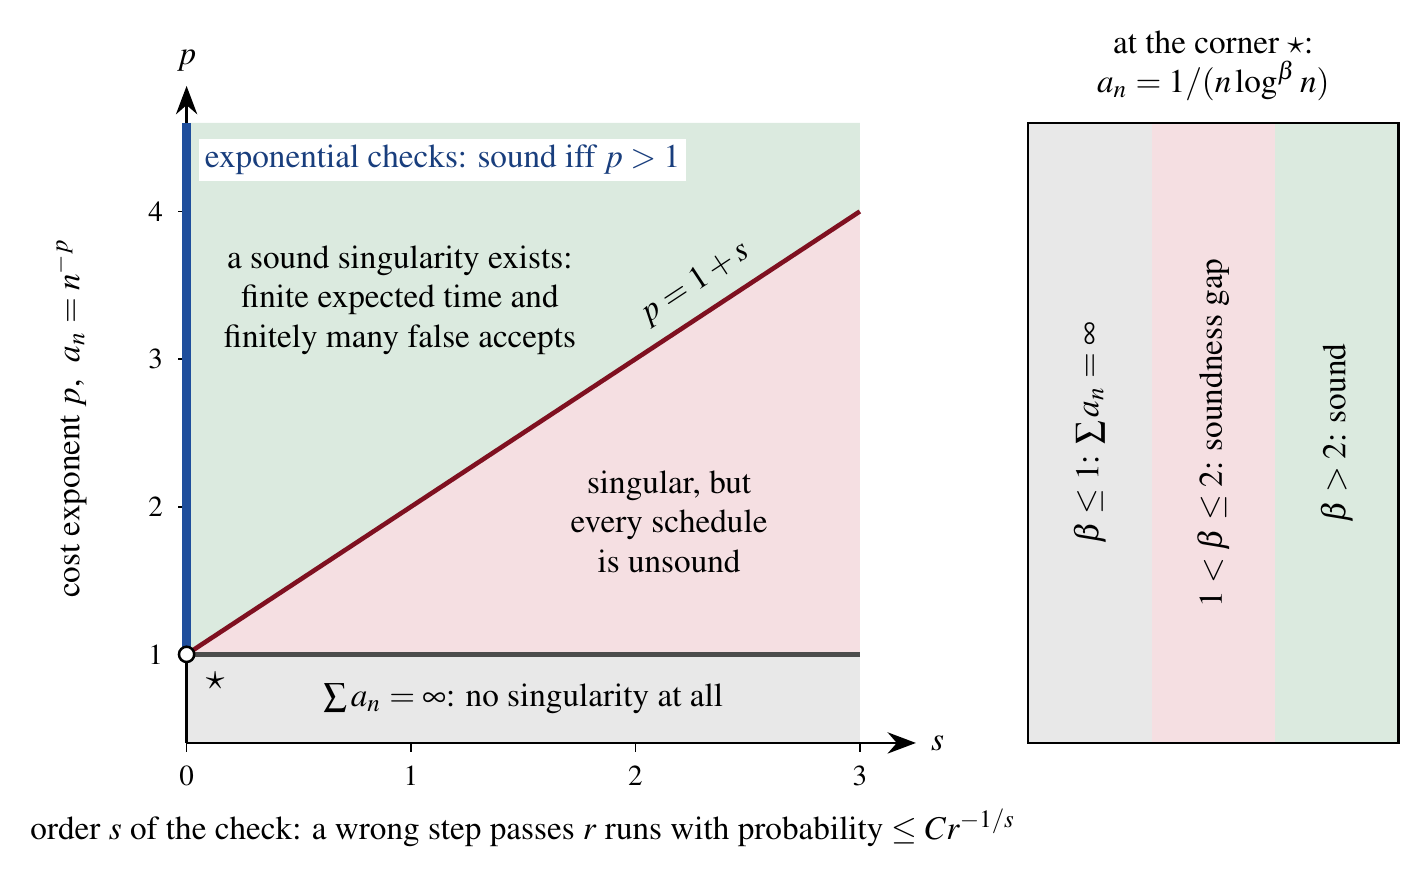
\includegraphics[width=0.86\textwidth]{figures/fig_regimes}
\caption{The phase diagram of Corollary~\ref{cor:phase} in the plane of the polynomial order $s$ of the checks and the exponent $p$ of the cost law $a_{n}=n^{-p}$. No singularity for $p\le1$; singular chains that are all unsound for $1<p\le1+s$; sound singular chains for $p>1+s$. The axis $s=0$ is the case of exponential checks, sound for every $p>1$. The panel at the corner refines the line $p=1$ by the logarithmic family $a_{n}=1/(n\log^{\beta}n)$ of Corollary~\ref{cor:gap}.}
\label{fig:regimes}
\end{figure*}

\section{Checking without knowing the future}\label{sec:online}

The schedules of Sections~\ref{sec:entropy} to~\ref{sec:singularity} are computed from the whole cost profile: the number of runs of the $i$-th check depends on $A$ and on every other cost. A self-improving system does not know its future modifications. When the $n$-th candidate arrives, only $a_{1},\dots,a_{n}$ are known, and the number of runs of its check must be fixed then. This section shows that such a system loses almost nothing: the entropy law survives with an additive term that grows like the logarithm of the logarithm of the dynamic range, and that term cannot be removed.

\subsection{Online schedules}

An \emph{online schedule} is a rule that assigns to each finite sequence $(a_{1},\dots,a_{n})$ of positive costs a number $r_{n}\in\NN$ of runs for the last candidate. Applied to a sequence $(a_{n})_{n\ge1}$, finite or infinite, it produces the schedule $(r_{n})$, and $r_{n}$ does not depend on $a_{n+1},a_{n+2},\dots$. The rule is \emph{$\theta$-sound} if $\sum_{n}\eps^{r_{n}}\le\theta$ for every sequence of positive costs. Write
\[
S_{n}=a_{1}+\dots+a_{n},\qquad u_{n}=\log\frac{S_{n}}{a_{1}},\qquad w_{n}=\frac{a_{n}/S_{n}}{2(1+u_{n})^{2}},
\]
so that $u_{1}=0$, $u_{n}$ is nondecreasing and $w_{1}=\frac12$. On the first $N$ candidates write $A_{N}=S_{N}$, $p^{(N)}=(a_{n}/A_{N})_{n\le N}$, $V_{N}=\sum_{n\le N}a_{n}r_{n}$ and $\Vs_{N}(\theta)$ for the offline optimum of Theorem~\ref{thm:A}.

\begin{mainthm}[Online entropy law]\label{thm:G}
Let $0<\eps<1$ and $0<\theta\le1$. The online schedule
\begin{equation}\label{eq:onlinerule}
r_{n}=\Bigl\lceil\frac1L\log\frac{1}{\theta w_{n}}\Bigr\rceil=\Bigl\lceil\frac1L\log\frac{2(1+u_{n})^{2}S_{n}}{\theta a_{n}}\Bigr\rceil
\end{equation}
is $\theta$-sound, and for every $N$
\begin{equation}\label{eq:onlineupper}
V_{N}\le\frac{A_{N}}{L}\Bigl(H(p^{(N)})+\log\frac1\theta+\log2+2\log\Bigl(1+\log\frac{A_{N}}{a_{1}}\Bigr)\Bigr)+A_{N}.
\end{equation}
Conversely, on the doubling costs $a_{n}=2^{n-1}$ every $\theta$-sound online schedule satisfies, for infinitely many $N$,
\begin{equation}\label{eq:onlinelower}
V_{N}-\Vs_{N}(\theta)\ \ge\ \frac{A_{N}}{2L}\log\log_{2}\Bigl(1+\frac{A_{N}}{a_{1}}\Bigr)-\Bigl(1+\frac{2\log2}{L}\Bigr)A_{N}.
\end{equation}
\end{mainthm}

Together with the lower bound of Theorem~\ref{thm:A}, \eqref{eq:onlineupper} says that the price of not knowing the future is at most $(A_{N}/L)(\log2+2\log(1+\log(A_{N}/a_{1})))+A_{N}$, and \eqref{eq:onlinelower} says that a term of order $(A_{N}/L)\log\log(A_{N}/a_{1})$ must be paid by every online rule on some sequences. The two bounds differ by a factor of four in the leading term. The dynamic range $A_{N}/a_{1}$ enters only through a double logarithm: a system whose total checking cost grows by a factor $10^{100}$ over its first candidate pays at most $2\log(1+100\log10)\approx10.9$ extra runs per unit of cost, measured in units of $L$.

\begin{corollary}[Sound singularities without foresight]\label{cor:onlinesing}
If $\sum_{n}a_{n}<\infty$ and $\sum_{n}a_{n}\log(1/a_{n})<\infty$, the online schedule \eqref{eq:onlinerule} is $\theta$-sound and has finite total cost
\[
V\le\frac{A}{L}\Bigl(H(p)+\log\frac1\theta+\log2+2\log\Bigl(1+\log\frac{A}{a_{1}}\Bigr)\Bigr)+A .
\]
\end{corollary}

So the criterion of Theorem~\ref{thm:E} does not need an oracle. A chain that only knows its past costs reaches a sound singularity whenever any chain does, and the rule that achieves it is the same for every sequence.

\subsection{Proofs}

The proof rests on two elementary facts, both proved in Lean (Appendix~\ref{app:checks}).

\begin{lemma}[Telescoping]\label{lem:telescope}
For $0\le x\le y$, $\dfrac{y-x}{(1+y)^{2}}\le\dfrac1{1+x}-\dfrac1{1+y}$. Hence for a nondecreasing sequence $0\le u_{1}\le u_{2}\le\cdots$,
\[
\sum_{n=2}^{N}\frac{u_{n}-u_{n-1}}{(1+u_{n})^{2}}\ \le\ \frac1{1+u_{1}}-\frac1{1+u_{N}}.
\]
\end{lemma}

\begin{proof}
The right side of the first inequality is $(y-x)/((1+x)(1+y))$, and $(1+x)\le(1+y)$. Summing gives a telescoping series.
\end{proof}

\begin{lemma}[Share of the newest cost]\label{lem:share}
For $0<s\le t$, $1-s/t\le\log(t/s)$. In particular $a_{n}/S_{n}=1-S_{n-1}/S_{n}\le u_{n}-u_{n-1}$ for $n\ge2$.
\end{lemma}

\begin{proof}
This is $1-1/x\le\log x$ at $x=t/s$, which is $\log y\le y-1$ at $y=1/x$. For the second statement take $s=S_{n-1}$, $t=S_{n}$ and note $\log(S_{n}/S_{n-1})=u_{n}-u_{n-1}$.
\end{proof}

\begin{proof}[Proof of Theorem~\ref{thm:G}]
\emph{Soundness.} By Lemma~\ref{lem:share} and Lemma~\ref{lem:telescope},
\[
\sum_{n=1}^{N}w_{n}=\frac12+\frac12\sum_{n=2}^{N}\frac{a_{n}/S_{n}}{(1+u_{n})^{2}}\le\frac12+\frac12\sum_{n=2}^{N}\frac{u_{n}-u_{n-1}}{(1+u_{n})^{2}}\le\frac12+\frac12\Bigl(1-\frac1{1+u_{N}}\Bigr)<1
\]
for every $N$ and every sequence of positive costs. Since $w_{n}\le\frac12<1$ and $\theta\le1$, the number inside the ceiling of \eqref{eq:onlinerule} is positive and $\eps^{r_{n}}\le\theta w_{n}$. Hence $\sum_{n}\eps^{r_{n}}\le\theta\sum_{n}w_{n}\le\theta$, and $r_{n}$ depends only on $a_{1},\dots,a_{n}$.

\emph{Cost.} From $r_{n}<\frac1L\log\frac1{\theta w_{n}}+1$,
\[
L\,V_{N}<\sum_{n\le N}a_{n}\Bigl(\log\frac1\theta+\log2+2\log(1+u_{n})+\log\frac{S_{n}}{a_{n}}\Bigr)+L\,A_{N}.
\]
For $n\le N$ we have $S_{n}\le A_{N}$, so $\log(S_{n}/a_{n})\le\log(A_{N}/a_{n})$ and $u_{n}\le\log(A_{N}/a_{1})$. Since $\sum_{n\le N}a_{n}\log(A_{N}/a_{n})=A_{N}H(p^{(N)})$, \eqref{eq:onlineupper} follows.

\emph{Lower bound.} Fix a $\theta$-sound online rule and apply it to the infinite sequence $a_{n}=2^{n-1}$. Its decisions on the first $N$ candidates are those it takes on the finite sequence $(a_{1},\dots,a_{N})$. Put $v_{n}=\eps^{r_{n}}/\theta$, so $\sum_{n}v_{n}\le1$. Then $v_{N}\le1/N$ for infinitely many $N$: otherwise $v_{N}>1/N$ for all large $N$ and $\sum v_{N}$ would diverge with the harmonic series. For such $N$, $r_{N}L\ge\log(N/\theta)$, and $r_{n}L\ge\log(1/\theta)$ for every $n$ because $\eps^{r_{n}}\le\theta$. Hence
\[
L\,V_{N}\ \ge\ A_{N}\log\frac1\theta+a_{N}\log N .
\]
On the other side, $p^{(N)}_{n}=2^{n-1}/(2^{N}-1)\ge2^{n-1-N}$, so
\[
H(p^{(N)})\le\log2\sum_{n=1}^{N}(N-n+1)\,p^{(N)}_{n}=\log2\cdot\frac{2^{N+1}-N-2}{2^{N}-1}\le2\log2,
\]
by the identity $\sum_{k=1}^{N}k2^{-k}=2-(N+2)2^{-N}$, and Theorem~\ref{thm:A} gives $L\,\Vs_{N}(\theta)\le A_{N}(2\log2+\log\frac1\theta)+LA_{N}$. Subtracting, and using $a_{N}=2^{N-1}\ge A_{N}/2$ and $N=\log_{2}(1+A_{N}/a_{1})$, gives \eqref{eq:onlinelower}.
\end{proof}

\begin{proof}[Proof of Corollary~\ref{cor:onlinesing}]
Soundness is that of Theorem~\ref{thm:G}. For the cost, the argument of the upper bound with $A$ in place of $A_{N}$ bounds every partial sum $V_{N}$ by the right side, since $S_{n}\le A$ for all $n$ and $\sum_{n\le N}a_{n}\log(A/a_{n})\le AH(p)$. The right side is finite because $AH(p)=A\log A+\sum_{n}a_{n}\log(1/a_{n})$.
\end{proof}

\subsection{Universal codes}

Theorem~\ref{thm:G} is the schedule counterpart of the universal codes for the integers. Elias constructed prefix codes whose length for the integer $m$ is $\log m+O(\log\log m)$ without knowledge of the distribution of $m$ \cite{Eli75}, and Rissanen derived from them a universal prior whose code length $\log^{\ast}m$ is optimal up to the iterated logarithms \cite{Ris83}. Here the role of the integer is played by the ratio $S_{n}/a_{1}$, the weight $w_{n}$ is a code length in disguise, and the double logarithm of \eqref{eq:onlineupper} is the price of the second level of the Elias code. The constant $2$ in front of it can be lowered to $1+\delta$ for every $\delta>0$ by replacing $(1+u_{n})^{2}$ with $c_{\delta}(1+u_{n})(1+\log(1+u_{n}))^{1+\delta}$, as in the Elias $\omega$ code; the lower bound \eqref{eq:onlinelower} shows that no rule removes the double logarithm.

Figure~\ref{fig:online} shows the rule at work. On random profiles its cost stays within the band of Theorem~\ref{thm:G}, and on the doubling sequence the excess over the offline optimum grows like $\log\log$ of the dynamic range, as the lower bound requires.

\begin{figure*}[t]
\centering
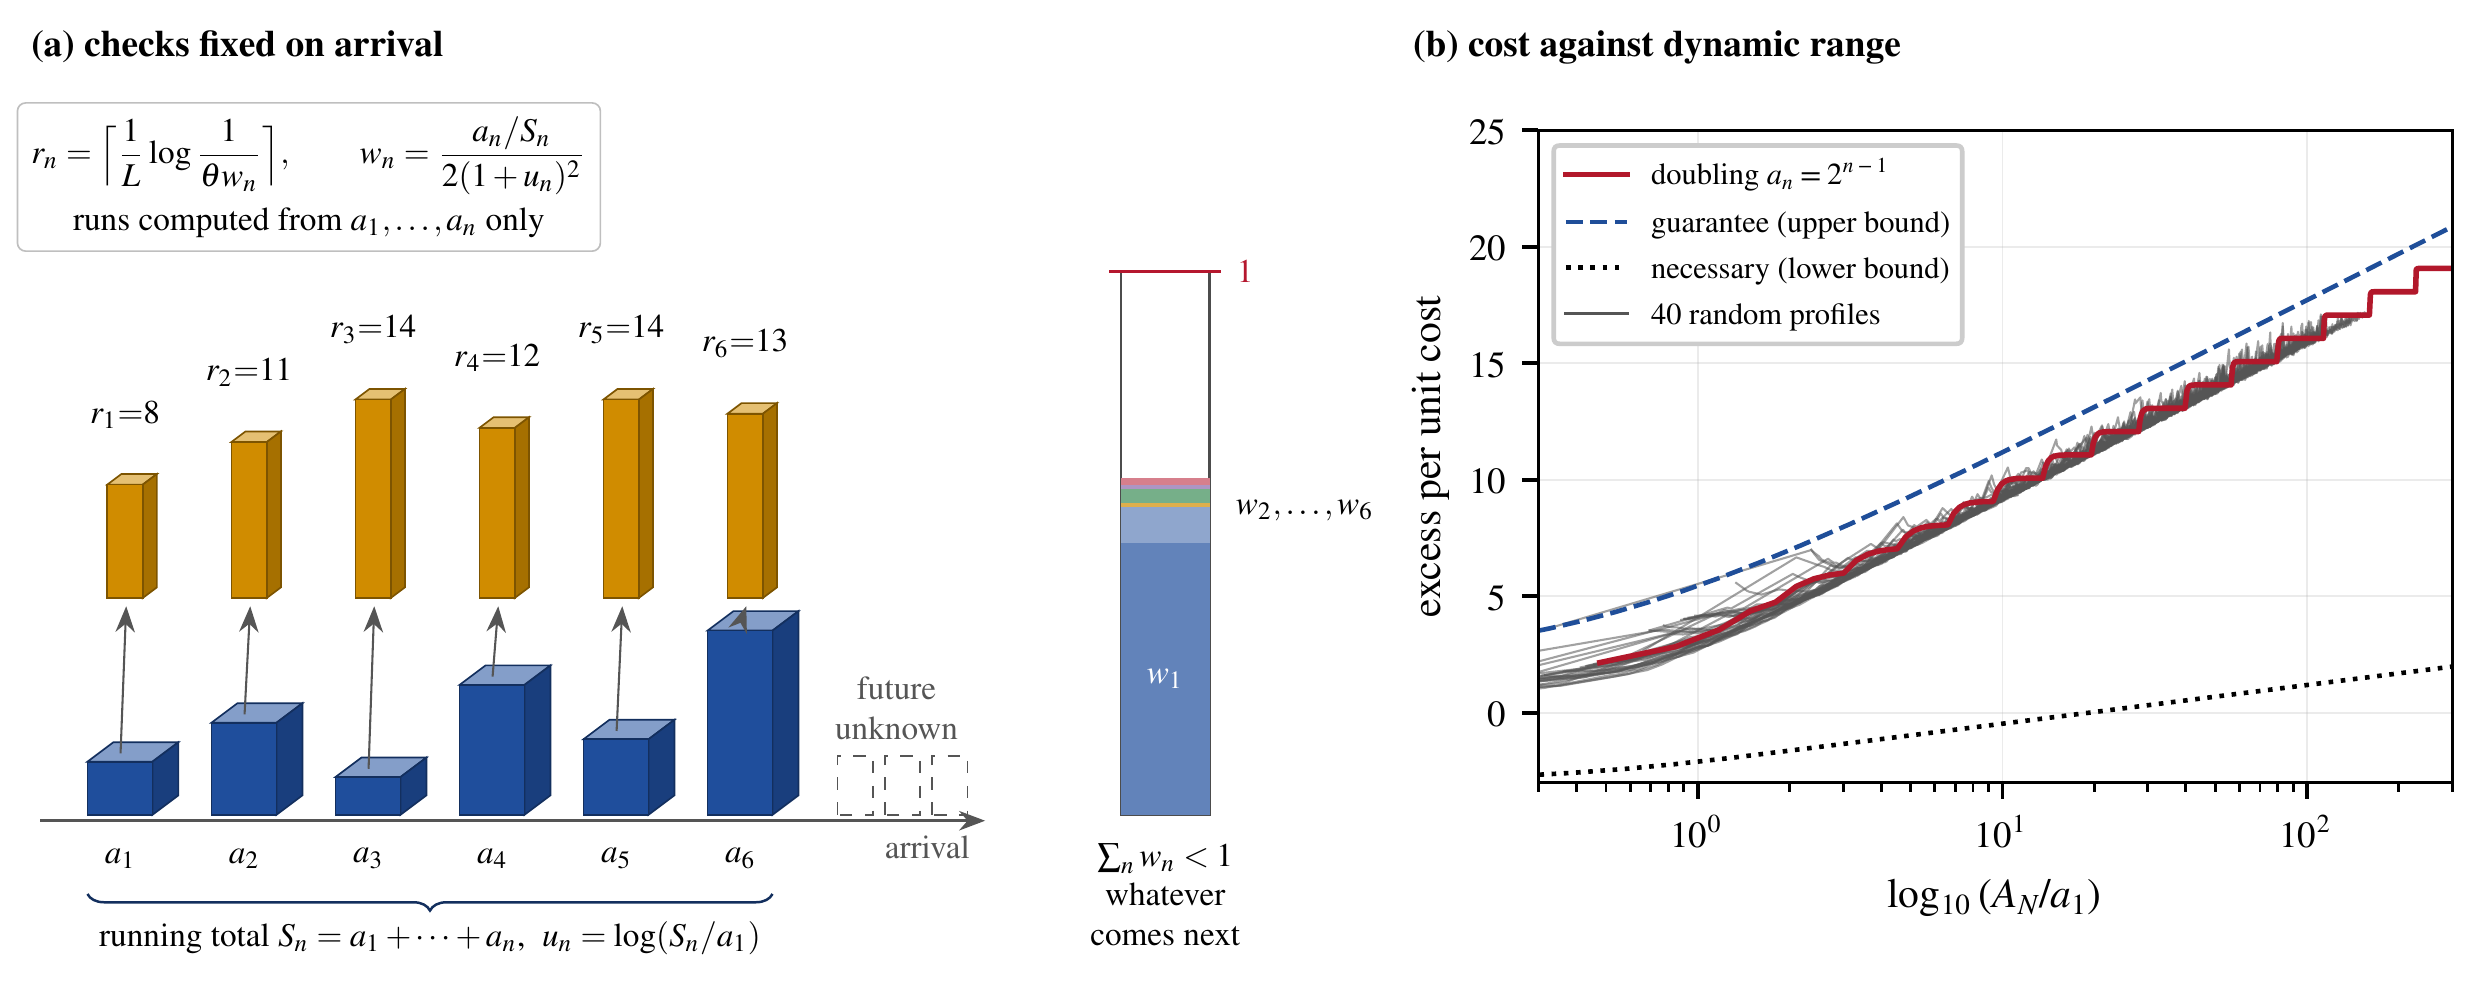
\includegraphics[width=0.98\textwidth]{figures/fig_online}
\caption{The online entropy law. (a) Candidates arrive one at a time; the $n$-th check is given $r_{n}$ runs computed from the running total $S_{n}$ alone, and the weights $w_{n}$ never sum to more than one, whatever comes next. (b) The excess $(V_{N}-\frac{A_{N}}{L}(H+\log\frac1\theta))/A_{N}$ of the online rule over the offline lower bound, for the doubling sequence $a_{n}=2^{n-1}$ (red) and for forty random profiles with log-normal costs (grey), against $\log_{10}(A_{N}/a_{1})$, with $\eps=\frac12$ and $\theta=10^{-6}$. The dashed curve is the guarantee $(\log2+2\log(1+\log(A_{N}/a_{1})))/L+1$ of \eqref{eq:onlineupper}, and the dotted curve is the necessary excess $\frac1{2L}\log\log_{2}(1+A_{N}/a_{1})-1-\frac{2\log2}{L}$ of \eqref{eq:onlinelower}.}
\label{fig:online}
\end{figure*}

\section{Subagents, cascades and the moves of a proof}\label{sec:agents}

A working BLLM is not one generator and one check. A coordinator hands parts of a problem to subagents, each subagent proposes candidates by its own method, and the candidates meet checks of very different cost: a test that runs in a millisecond, a randomized identity test, a full proof checker. This section proves the two laws that govern such a system. Splitting the work among subagents costs nothing, provided each receives a share of the budget proportional to its total cost, and a misallocated budget is charged exactly a Kullback--Leibler divergence (Theorem~\ref{thm:H}). Cheap unreliable checks placed before an exact one make the exact check paid, up to a logarithmic premium, only on the correct candidates (Theorem~\ref{thm:cascade}). The section ends with the six moves by which the subagents of Section~\ref{sec:cases} propose candidates.

\subsection{Subagents}

Partition the candidates into groups $G_{1},\dots,G_{m}$, one for each subagent. Write $A_{k}=\sum_{i\in G_{k}}a_{i}$, $P_{k}=A_{k}/A$ for the share of the $k$-th subagent and $p^{(k)}=(a_{i}/A_{k})_{i\in G_{k}}$ for its own cost profile. A coordinator gives the $k$-th subagent a budget $\theta_{k}>0$ with $\Theta=\sum_{k}\theta_{k}\le\theta$, and the subagent schedules its checks with any $\theta_{k}$-sound schedule. The union of the schedules is $\theta$-sound, since the expected numbers of false acceptances add.

\begin{mainthm}[Subagents]\label{thm:H}
\begin{enumerate}[label=\textup{(\roman*)},leftmargin=2.2em,itemsep=1pt]
\item \emph{Chain rule.} $H(p)=H(P)+\sum_{k}P_{k}H(p^{(k)})$.
\item \emph{Price of a split.} The sum over the subagents of the lower bounds of Theorem~\ref{thm:A} for their groups exceeds the lower bound for the whole profile by exactly
\begin{equation}\label{eq:splitprice}
\frac{A}{L}\Bigl(D(P\,\|\,q)+\log\frac{\theta}{\Theta}\Bigr),\qquad q_{k}=\frac{\theta_{k}}{\Theta},
\end{equation}
where $D$ is the Kullback--Leibler divergence. It vanishes if and only if $\theta_{k}=\theta P_{k}$ for every $k$.
\item \emph{Coordination by one number.} If $\theta_{k}=\theta P_{k}$, the optimal schedule of Theorem~\ref{thm:A} computed by the $k$-th subagent from its own costs and the single number $\theta P_{k}$ coincides on $G_{k}$ with the optimal schedule of the whole profile. The union is $\theta$-sound and costs at most $\frac AL(H(p)+\log\frac1\theta)+A$.
\item \emph{Hierarchies.} For a tree of subagents in which every node passes to each child the share of its own budget proportional to the child's total cost, the schedule at the leaves is the optimal flat schedule, and
\begin{equation}\label{eq:treeentropy}
A\,H(p)=\sum_{v}A_{v}\,H(P^{v}),
\end{equation}
the sum over the internal nodes $v$ of the tree, where $A_{v}$ is the total cost below $v$ and $P^{v}$ the distribution of $A_{v}$ among the children of $v$.
\end{enumerate}
\end{mainthm}

\begin{proof}
(i) For $i\in G_{k}$, $\log(A/a_{i})=\log(A/A_{k})+\log(A_{k}/a_{i})$; multiply by $a_{i}$, sum over $i\in G_{k}$ and then over $k$, and divide by $A$.

(ii) The lower bounds for the groups add up to $\frac1L\sum_{k}\bigl(A_{k}H(p^{(k)})+A_{k}\log\frac1{\theta_{k}}\bigr)$. By (i), subtracting $\frac AL(H(p)+\log\frac1\theta)$ leaves
\[
\frac1L\Bigl(\sum_{k}A_{k}\log\frac1{\theta_{k}}-A\,H(P)-A\log\frac1\theta\Bigr)=\frac AL\sum_{k}P_{k}\log\frac{\theta P_{k}}{\theta_{k}}=\frac AL\Bigl(\sum_{k}P_{k}\log\frac{P_{k}}{q_{k}}+\log\frac\theta\Theta\Bigr).
\]
Both terms are nonnegative, the first by Gibbs' inequality (Lemma~\ref{lem:gibbs}), and they vanish together exactly when $q=P$ and $\Theta=\theta$, that is, when $\theta_{k}=\theta P_{k}$.

(iii) The ceiling schedule of the $k$-th group at budget $\theta P_{k}$ gives $i\in G_{k}$ the number of runs $\lceil\frac1L\log\frac{A_{k}}{\theta P_{k}a_{i}}\rceil=\lceil\frac1L\log\frac{A}{\theta a_{i}}\rceil$, which is the flat ceiling schedule; its soundness and cost are those of Theorem~\ref{thm:A}.

(iv) By induction on the depth, applying (iii) at the root and the induction hypothesis to each subtree with its proportional budget. The identity \eqref{eq:treeentropy} follows by applying (i) at every internal node.
\end{proof}

The theorem has a practical reading. A coordinator need not know the costs of the individual checks of its subagents, and a subagent need not know anything about the others: one number per subagent, its share $\theta P_{k}$ of the budget, is enough to reach the global optimum, and the identity \eqref{eq:treeentropy} says that the entropy tax is paid node by node along the tree of delegation, each node paying for the uncertainty of its own split. A coordinator that splits the budget evenly among $m$ subagents instead pays the extra $\frac AL D(P\,\|\,u)=\frac AL(\log m-H(P))$, where $u$ is uniform, and this is unbounded when a few subagents carry almost all the cost.

\subsection{Weak checks before strong ones}

Let a fraction $\rho\in(0,1)$ of the candidates be incorrect. A \emph{strong check} costs $c$ and is exact: it accepts the correct candidates and rejects the others, as a proof checker does on a formal proof. A \emph{weak check} costs $b$ per run, has perfect completeness and soundness $\eps$: a language model asked to find a flaw, a numerical test at random points, a type check. A \emph{cascade} with $r$ weak runs runs the weak check $r$ times on every candidate and the strong check on the candidates that pass them. It keeps exactly the correct candidates, whatever $r$, so its soundness is that of the strong check alone.

\begin{theorem}[Weak before strong]\label{thm:cascade}
If the weak check attains its soundness, the expected cost of a cascade with $r$ weak runs per candidate is
\[
E(r)=br+c(1-\rho)+c\rho\,\eps^{r},
\]
and for $b\le c\rho L$,
\begin{equation}\label{eq:cascade}
c(1-\rho)+\frac bL\Bigl(1+\log\frac{c\rho L}{b}\Bigr)\ \le\ \min_{r\in\NN}E(r)\ \le\ c(1-\rho)+\frac bL\Bigl(1+\log\frac{c\rho L}{b}\Bigr)+b,
\end{equation}
the upper bound being attained up to $b$ by $r=\lceil\frac1L\log\frac{c\rho L}{b}\rceil$. Without weak checks the cost is $c$.
\end{theorem}

\begin{proof}
A correct candidate passes the $r$ weak runs and reaches the strong check; an incorrect one reaches it with probability $\eps^{r}$. This gives $E(r)$. Put $y=c\rho\eps^{r}$, so that $r=\frac1L\log\frac{c\rho}{y}$ and
\[
br+c\rho\eps^{r}-\frac bL\Bigl(1+\log\frac{c\rho L}{b}\Bigr)=\frac bL\Bigl(\frac{yL}{b}-1-\log\frac{yL}{b}\Bigr)\ge0
\]
by $\log x\le x-1$. This is the lower bound. For the upper bound let $x=\frac1L\log\frac{c\rho L}{b}\ge0$ and $r=\lceil x\rceil$. Then $br\le bx+b$ and $\eps^{r}\le\eps^{x}=b/(c\rho L)$, so $c\rho\eps^{r}\le b/L$.
\end{proof}

The strong check is thus paid on a fraction $1-\rho$ of the candidates, the correct ones, plus a premium logarithmic in $c/b$. When most proposals are wrong, as for a language model that guesses the next step of a hard proof, the saving is close to the factor $1/(1-\rho)$. With a proof checker of cost $c=1000$, a weak check of cost $b=1$ and soundness $\frac12$, and nine proposals in ten wrong, the best cascade runs nine weak checks per candidate and costs $110.8$ against $1000$; the lower bound is $110.7$.

The proof shows something more important than the saving. The soundness of the cascade does not depend on $\eps$: a weak check, however unreliable, can only remove candidates, never admit one. A learned critic may therefore be used freely as a filter, and only as a filter; the decision belongs to the exact check. The same holds with a randomized strong check of soundness $\eps_{s}$ given $r_{s}$ runs, whose false acceptances are bounded by $\rho\eps^{r}\eps_{s}^{r_{s}}\le\rho\eps_{s}^{r_{s}}$, so the weak runs may also be counted towards the budget of Theorem~\ref{thm:A} but are never needed for it.

\subsection{The moves of a proof}\label{ssec:moves}

The formal proofs of Section~\ref{sec:cases} are built from a small number of moves, used over and over. We name six, and the BLLM package of Section~\ref{sec:cases} has one subagent for each. A move is a way of generating candidates; it carries no authority of its own, and every candidate it produces meets the same checks, so Theorems~\ref{thm:A} to~\ref{thm:H} and~\ref{thm:cascade} apply to any mixture of moves.

\emph{Construction} produces an explicit object, a flow, a lattice, a cycle, a schedule, together with the statement that it has the required property, which is then checked. \emph{Strong then weak} proposes the strongest statement first and, when it is rejected, the next rung of a ladder of weakenings: a special case, a bounded range, a conditional form. Each rung is a candidate and enters the cost profile of Theorem~\ref{thm:A}. \emph{Residual} turns a partial success into a new goal, the part that remains unproved; it is the retry of Theorem~\ref{thm:B}, and when the corrections go on without end, as in a construction corrected to every order, whether the infinite sequence can be certified at finite cost is decided by Theorem~\ref{thm:E} and, without knowledge of the future corrections, by Corollary~\ref{cor:onlinesing}. \emph{Trivialization} specialises the parameters of a goal until it becomes a finite computation, which a kernel decides exactly, so that its check has soundness zero. \emph{Bypass} replaces a step by a result already kept in memory, whose check has been paid once. \emph{Blow-up} searches for a singular object or a counterexample.

\begin{remark}[Refutations carry no entropy tax]\label{rem:refutation}
A counterexample checked by exact evaluation needs one run, whatever the budget, because its check has soundness zero; so do the finite computations produced by trivialization and the results reused by bypass. In a mixed profile the entropy of Theorem~\ref{thm:A} is therefore the entropy of the candidates whose checks are randomized, with total cost $A_{\mathrm{rand}}$, and the exact checks add their cost once. A system that turns more of its work into exact checks lowers both $A_{\mathrm{rand}}$ and the entropy it pays on it.
\end{remark}

Figure~\ref{fig:agents} shows the arrangement: a coordinator, six subagents, a cascade of weak and strong checks, and a memory that stores every kept result as a note linked to the results it uses.

\begin{figure*}[t]
\centering
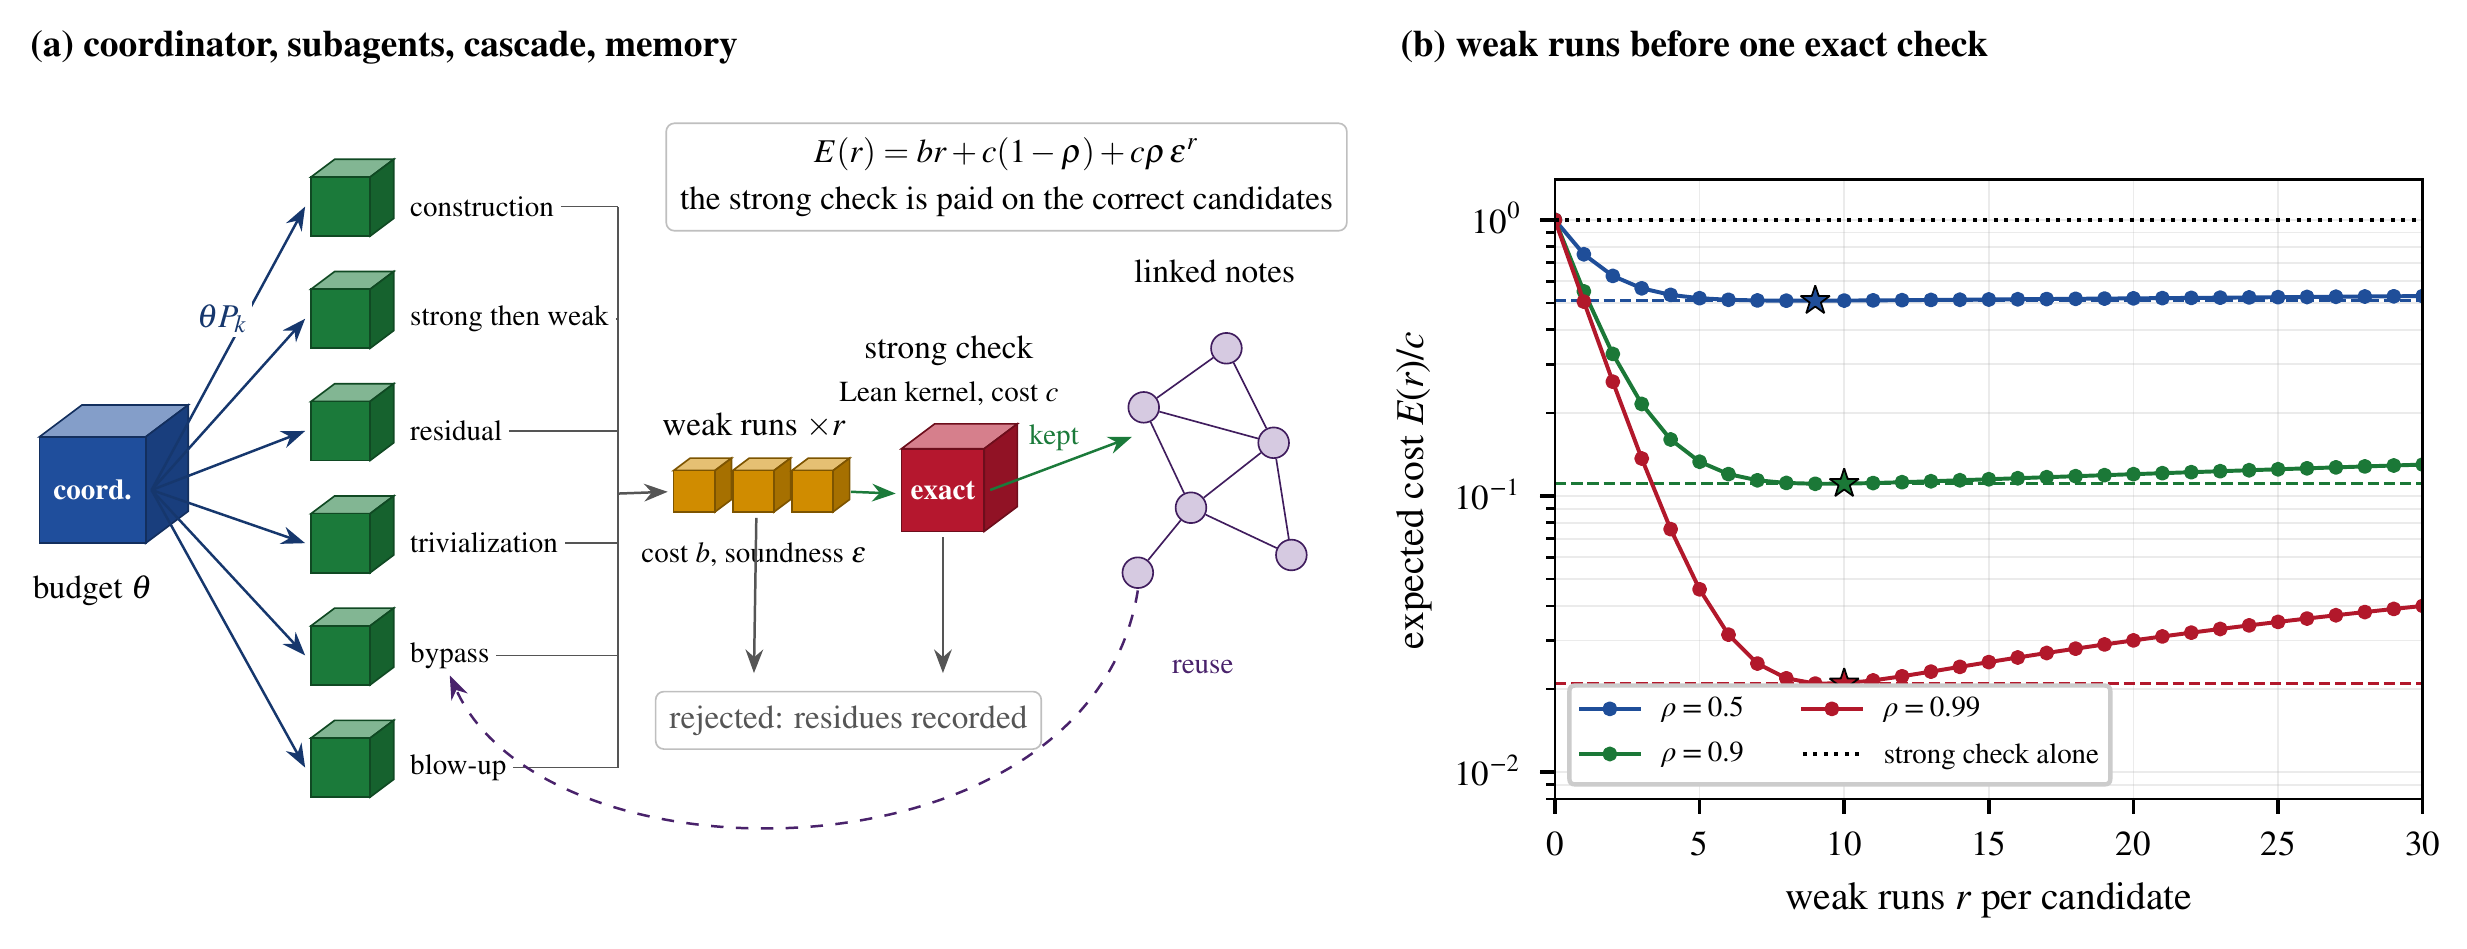
\includegraphics[width=0.98\textwidth]{figures/fig_agents}
\caption{Subagents and cascades. (a) A coordinator passes to each of six subagents, one for each move of Section~\ref{ssec:moves}, the share $\theta P_{k}$ of the budget proportional to its total cost (Theorem~\ref{thm:H}); every candidate meets a cascade of $r$ weak runs and one exact strong check (Theorem~\ref{thm:cascade}), and the kept results are stored as linked notes that the bypass move reuses. (b) The expected cost $E(r)/c$ of a cascade against the number $r$ of weak runs, for $b/c=10^{-3}$, $\eps=\frac12$ and $\rho\in\{0.5,0.9,0.99\}$; stars mark the number of runs of Theorem~\ref{thm:cascade}, the lower bound of \eqref{eq:cascade} is dashed and the cost $1$ of the strong check alone dotted.}
\label{fig:agents}
\end{figure*}

\section{Branching takeoff}\label{sec:branching}

\subsection{The tree of improvements}

A self-improving system need not move along a chain. Each kept improvement may spawn several candidates for the next, and the improvements form a tree (Fig.~\ref{fig:branchtree}). The model is a Galton--Watson process with checks.

\begin{definition}[Checked branching process]\label{def:branching}
Generation $0$ is one kept correct system. Each kept correct improvement of generation $k-1$ spawns an independent copy of a random number $\xi\ge0$ of candidates, with $\EE\,\xi=\mu$ and $\PR(\xi\ge1)>0$. Each candidate is correct with probability $\gamma\in(0,1)$, independently. The check of generation $k$ keeps a correct candidate with probability $1-\eta$ and an incorrect one with probability $\delta_{k}\in(0,1]$. Kept incorrect candidates are quarantined: they spawn nothing. Let $Z_{k}$ be the number of kept correct improvements of generation $k$, $F_{k}$ the number of kept incorrect ones, $F=\sum_{k\ge1}F_{k}$, and $m=\mu\gamma(1-\eta)$.
\end{definition}

The number $N$ of kept correct offspring of one kept correct improvement is obtained from $\xi$ by keeping each candidate independently with probability $\gamma(1-\eta)$, so $(Z_{k})$ is a Galton--Watson process with offspring law $N$ and mean $\EE N=m$. If $\xi$ is Poisson with mean $\mu$, then $N$ is Poisson with mean $m$. The quarantine assumption is needed only for the formula for $\EE F$; without it $F$ is larger, so the statements that force $F=\infty$ hold a fortiori.

\begin{figure*}[t]
\centering
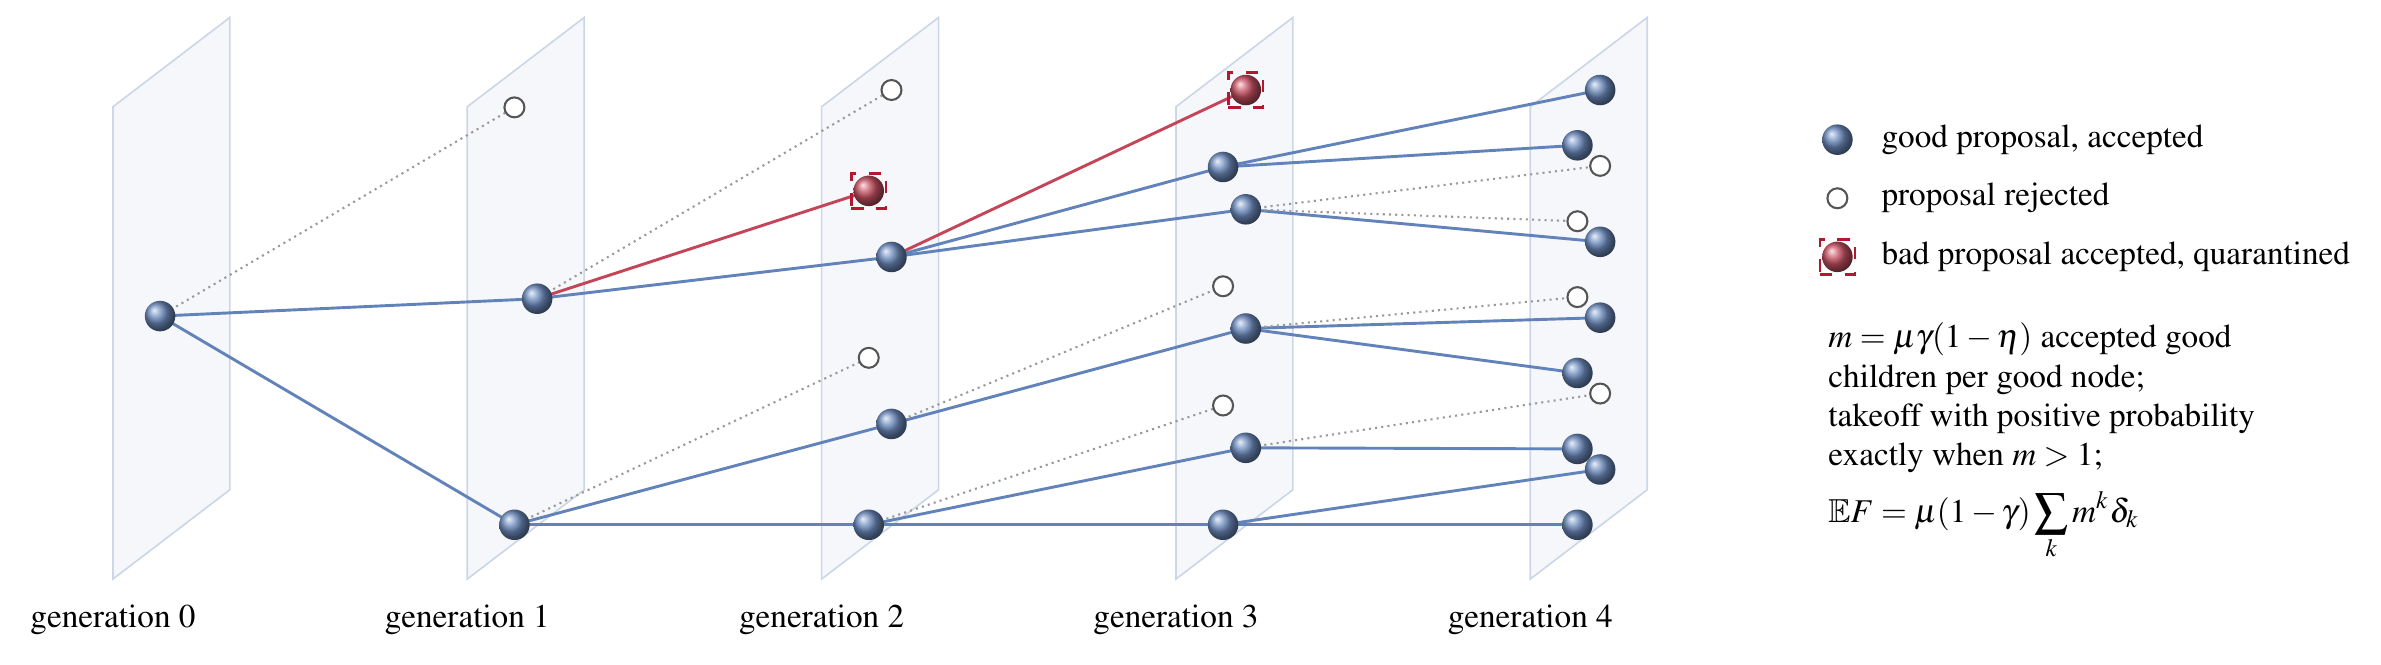
\includegraphics[width=0.92\textwidth]{figures/fig_branchtree}
\caption{A checked branching process, Definition~\ref{def:branching}, over four generations drawn as sheets. Blue nodes are kept correct improvements, which spawn the next generation; grey nodes are rejected candidates; red nodes are incorrect candidates that the check kept, which are quarantined. The kept correct improvements grow like $m^{k}$ in mean, and the expected number of kept errors is $\mu(1-\gamma)\sum_{k}m^{k-1}\delta_{k}$ (Theorem~\ref{thm:F}).}
\label{fig:branchtree}
\end{figure*}

\subsection{Takeoff}

The process \emph{takes off} if $Z_{k}>0$ for every $k$. Let $f(z)=\EE\,z^{N}$ and $q=\PR(\text{takeoff})$.

\begin{proposition}[Takeoff threshold]\label{prop:takeoff}
Assume $\PR(N=1)<1$. Then $q>0$ if and only if $m>1$, and $1-q$ is the least root of $f(z)=z$ in $[0,1]$. If moreover $\EE N^{2}<\infty$ and $m>1$, then
\[
\frac{2(m-1)}{f''(1)}\ \le\ q\ \le\ \frac{2(m-1)}{f''(1-q)} .
\]
For Poisson offspring, $f''(1)=m^{2}$, $f''(1-q)=m^{2}(1-q)$ and, for $1<m\le2$, $\bigl|q-2(m-1)/m^{2}\bigr|\le4e^{4}(m-1)^{2}$.
\end{proposition}

\begin{proof}
The first two claims are the classical extinction theorem \cite{AN72,WG75}; Appendix~\ref{app:gw} recalls the proof. For the bounds, Taylor's formula at $1$ with $f(1)=1$ and $f'(1)=m$ gives $f(1-q)=1-mq+\frac12f''(\xi)q^{2}$ for some $\xi\in(1-q,1)$. Since $f(1-q)=1-q$, this is $(m-1)q=\frac12f''(\xi)q^{2}$, so $q=2(m-1)/f''(\xi)$; and $f''$ is increasing on $[0,1]$, being a power series with nonnegative coefficients, so $f''(1-q)\le f''(\xi)\le f''(1)$. For Poisson offspring $f(z)=e^{m(z-1)}$, $f''(z)=m^{2}e^{m(z-1)}$, and $e^{-mq}=1-q$ at the fixed point. The two bounds then differ by $\frac{2(m-1)}{m^{2}}\cdot\frac{q}{1-q}$. Extinction has probability at least $\PR(N=0)=e^{-m}\ge e^{-2}$, so $1-q\ge e^{-2}$ and $q\le2e^{2}(m-1)$; the difference is at most $2(m-1)e^{2}\cdot2e^{2}(m-1)$.
\end{proof}

Near the threshold the probability of takeoff is linear in $m-1$, with slope $2/f''(1)$, which tends to $2/\sigma^{2}$ at criticality, $\sigma^{2}$ the variance of the offspring law there; Table~\ref{tab:gw} gives the numbers for Poisson offspring and Fig.~\ref{fig:branching}(a) the curves. A takeoff is never certain: for $m\le2$ it fails with probability at least $e^{-2}$, and it is a matter of luck in its first generations.

\begin{table}[b]
\caption{Probability $q$ of takeoff for Poisson offspring of mean $m$, with the two bounds of Proposition~\ref{prop:takeoff}.}
\label{tab:gw}
\centering
\small
\begin{tabular}{@{}c c c c@{}}
\toprule
$m$ & $2(m-1)/m^{2}$ & $q$ & $2(m-1)/(m^{2}(1-q))$ \\
\midrule
$1.02$ & $0.0385$ & $0.0390$ & $0.0400$ \\
$1.05$ & $0.0907$ & $0.0937$ & $0.1001$ \\
$1.10$ & $0.1653$ & $0.1761$ & $0.2006$ \\
$1.20$ & $0.2778$ & $0.3137$ & $0.4048$ \\
$1.50$ & $0.4444$ & $0.5828$ & $1.0653$ \\
$2.00$ & $0.5000$ & $0.7968$ & $2.4608$ \\
\bottomrule
\end{tabular}
\end{table}

\subsection{Errors in a takeoff}

\begin{proof}[Proof of Theorem~\ref{thm:F}]
\emph{Threshold.} This is Proposition~\ref{prop:takeoff}.

\emph{Expected errors.} Let $\mathcal F_{k}$ be the information of generations $0,\dots,k$. Given $\mathcal F_{k-1}$, the $Z_{k-1}$ kept correct improvements spawn on average $\mu Z_{k-1}$ candidates, each incorrect and kept with probability $(1-\gamma)\delta_{k}$, so $\EE[F_{k}\mid\mathcal F_{k-1}]=\mu(1-\gamma)\delta_{k}Z_{k-1}$. With $\EE Z_{k-1}=m^{k-1}$ and monotone convergence, $\EE F=\mu(1-\gamma)\sum_{k\ge1}m^{k-1}\delta_{k}$. If the series converges, $F<\infty$ almost surely.

\emph{Divergence.} Let $m>1$, $\EE\,\xi\log\xi<\infty$ and $\sum m^{k-1}\delta_{k}=\infty$. Since $N\le\xi$, also $\EE N\log N<\infty$, and the Kesten--Stigum theorem \cite{KS66,AN72} gives $Z_{k}/m^{k}\to W$ almost surely with $W>0$ almost surely on takeoff. Let $B_{k}=\{F_{k}\ge1\}\in\mathcal F_{k}$ and $u_{k}=(1-\gamma)\delta_{k}$. Given $\mathcal F_{k-1}$ the parents act independently, and one parent with $\xi$ candidates keeps no incorrect one with probability $\EE(1-u_{k})^{\xi}\le1-u_{k}\PR(\xi\ge1)$, because $1-(1-u)^{j}\ge u$ for $j\ge1$. With $c_{0}=\PR(\xi\ge1)>0$,
\[
\begin{aligned}
\PR(B_{k}\mid\mathcal F_{k-1})&\ \ge\ 1-(1-c_{0}u_{k})^{Z_{k-1}}\ \ge\ 1-e^{-c_{0}u_{k}Z_{k-1}}\\
&\ \ge\ \tfrac12\min(c_{0}u_{k}Z_{k-1},1),
\end{aligned}
\]
the last step by $1-e^{-x}\ge\frac12\min(x,1)$. On takeoff, $Z_{k-1}\ge\frac12Wm^{k-1}$ for all large $k$, so up to finitely many terms
\[
\sum_{k}\PR(B_{k}\mid\mathcal F_{k-1})\ge\frac12\sum_{k}\min\Bigl(\frac{c_{0}(1-\gamma)W}{2}\,m^{k-1}\delta_{k},\,1\Bigr).
\]
 The right side diverges, since $\sum m^{k-1}\delta_{k}$ diverges and a series $\sum\min(cx_{k},1)$ with $c>0$, $x_{k}\ge0$ converges only if $\sum x_{k}$ does. L\'evy's conditional Borel--Cantelli lemma \cite{Dur19} states that $\{B_{k}\text{ infinitely often}\}$ and $\{\sum_{k}\PR(B_{k}\mid\mathcal F_{k-1})=\infty\}$ agree up to a null set (Appendix~\ref{app:levy}). So $F=\infty$ almost surely on takeoff.

\emph{Exponential checks.} With $\delta_{k}=\eps^{r_{k}}$ and $r_{k}=\lceil k\log(2m)/L\rceil$, $r_{k}L\ge k\log(2m)$, so $m^{k}\eps^{r_{k}}\le2^{-k}$ and $\sum m^{k-1}\delta_{k}\le\frac1m\sum2^{-k}<\infty$. Conversely, if $\sum m^{k-1}\eps^{r_{k}}<\infty$, its terms tend to $0$, so $r_{k}L-(k-1)\log m\to\infty$, hence $r_{k}L\ge k\log m$ for all large $k$. A constant $\delta_{k}=\delta>0$ gives $\sum m^{k-1}\delta=\infty$ for $m\ge1$.
\end{proof}

\begin{corollary}[The entropy tax of a takeoff]\label{cor:branchtax}
In a sound takeoff with exponential checks and $m>1$, every kept correct improvement of generation $k$ has been checked by at least $k\log m/L=\log(\EE Z_{k})/L$ runs, for all large $k$.
\end{corollary}

The tax is the logarithm of the size of the population, divided by $L$, exactly as for $n$ candidates of equal cost in Corollary~\ref{cor:uniform}: a growing population of improvements can stay sound only if each new improvement is checked harder than the last by a fixed number of runs per generation, and a fixed false acceptance rate, however small, lets errors multiply with the population (Fig.~\ref{fig:branching}(b)).

\begin{figure*}[t]
\centering
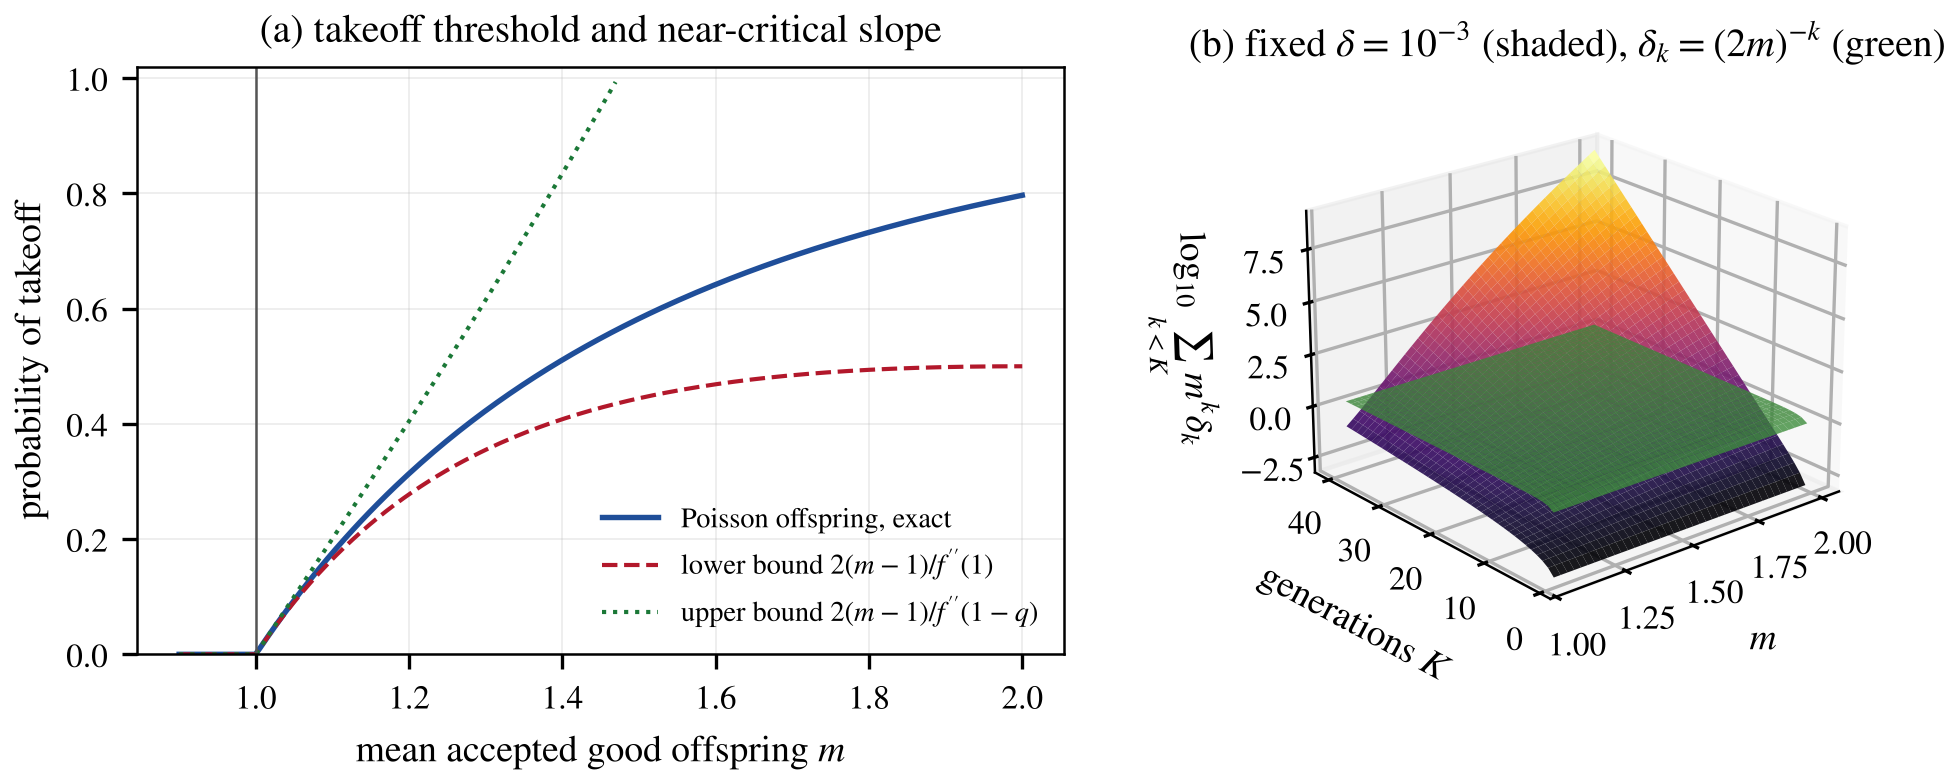
\includegraphics[width=0.98\textwidth]{figures/fig_branching}
\caption{Theorem~\ref{thm:F}. (a) The probability of takeoff for Poisson offspring as a function of the mean $m$ of kept correct offspring, with the two bounds of Proposition~\ref{prop:takeoff}; the threshold is $m=1$ and the slope there is $2$. (b) The expected number of kept errors in the first $K$ generations, $\log_{10}\sum_{k<K}m^{k}\delta_{k}$, for a fixed rate $\delta=10^{-3}$ (shaded surface), which grows without bound, and for the amplified rate $\delta_{k}=(2m)^{-k}$ (green), which stays below $\log_{10}2$.}
\label{fig:branching}
\end{figure*}

\section{Growth laws and the price of a sound takeoff}\label{sec:scaling}

\subsection{Osgood takeoffs}

Theorems~\ref{thm:E} and~\ref{thm:F} take the costs $a_{n}$ as given. Growth models of an intelligence explosion produce them. The simplest such model, and the one behind most informal arguments, is the equation
\[
\frac{dI}{dt}=c\,I^{\alpha},\qquad c>0,\ \alpha>0,
\]
for a capability $I$ that speeds up its own improvement. Its solution from $I(0)=1$ reaches infinity at the finite time $\int_{1}^{\infty}dI/(cI^{\alpha})=1/(c(\alpha-1))$ when $\alpha>1$ and grows without blowing up when $\alpha\le1$; Osgood's criterion states the same for $dI/dt=f(I)$ with the integral of $1/f$ \cite{Osg98}.\footnote{W.~F. Osgood, \emph{Beweis der Existenz einer L\"osung der Differentialgleichung $dy/dx=f(x,y)$ ohne Hinzunahme der Cauchy--Lipschitzschen Bedingung}, Monatshefte f\"ur Mathematik und Physik 9 (1898), 331--345 \cite{Osg98}. The paper is about uniqueness; the blow-up criterion that bears Osgood's name is the elementary fact, implicit there, that a solution of $y'=f(y)$ with $f>0$ reaches infinity in the finite time $\int_{y_{0}}^{\infty}dy/f(y)$ exactly when the integral converges. For $f(y)=cy^{\alpha}$ the integral is $y_{0}^{1-\alpha}/(c(\alpha-1))$ for $\alpha>1$ and diverges for $\alpha\le1$.} To put a check on the curve one has to say what one improvement is. Two choices are natural.

\emph{Additive steps.} The $n$-th improvement raises the capability from $n$ to $n+1$ at the rate reached at its start, so it takes the time $g_{n}=1/(cn^{\alpha})$.

\emph{Multiplicative steps.} The $n$-th improvement multiplies the capability by a fixed factor $\lambda>1$, from $\lambda^{n-1}$ to $\lambda^{n}$, at the rate reached at its start, so it takes the time $g_{n}=(\lambda-1)\lambda^{n-1}/(c\lambda^{(n-1)\alpha})=\frac{\lambda-1}{c}\,q^{n-1}$ with $q=\lambda^{-(\alpha-1)}$.

In both cases we let the check of the $n$-th improvement cost a fixed fraction $\kappa>0$ of the time it took to make, $a_{n}=\kappa g_{n}$ per run, so that faster improvements are also faster to check. Write $G=\sum_{n}g_{n}$ for the unchecked takeoff time and $T_{\theta}=G+\Vs(\theta)$ for the least time of a takeoff with at most $\theta$ expected false acceptances, measured, as in Theorem~\ref{thm:A}, in the run in which every candidate is correct.

\begin{proposition}[Osgood takeoffs]\label{prop:osgood}
Let $\alpha>1$, $0<\theta\le1$ and $0<\eps<1$.
\begin{enumerate}[label=\textup{(\roman*)},leftmargin=2.2em,itemsep=1pt]
\item In both models
\[
\begin{aligned}
\frac{T_{\theta}}{G}&\ge 1+\frac{\kappa}{L}\Bigl(H+\log\frac1\theta\Bigr),\\
\frac{T_{\theta}}{G}&\le 1+\frac{\kappa}{L}\Bigl(H+\log\frac1\theta\Bigr)+\kappa ,
\end{aligned}
\]
where $H$ is the entropy of the profile $g/G$.
\item For additive steps $G=\zeta(\alpha)/c$, which lies between $1/(c(\alpha-1))$ and $\alpha/(c(\alpha-1))$, and, as $\alpha\to1^{+}$,
\[
H=\frac1{\alpha-1}+\log\frac1{\alpha-1}+O(1).
\]
Hence the least check time of a sound takeoff is
\[
T_{\theta}-G=\frac{\kappa\bigl(1+O\bigl((\alpha-1)\log\frac1{\alpha-1}\bigr)\bigr)}{c(\alpha-1)^{2}L}.
\]
\item For multiplicative steps $G=(\lambda-1)/(c(1-q))$ and
\[
\begin{aligned}
H&=\log\frac1{1-q}+\frac{q}{1-q}\log\frac1q\\
&=\log\frac1{(\alpha-1)\log\lambda}+1+o(1)\qquad(\alpha\to1^{+}).
\end{aligned}
\]
Hence
\[
T_{\theta}-G=\frac{\kappa}{c(\alpha-1)L}\cdot\frac{\lambda-1}{\log\lambda}\Bigl(\log\frac1{\alpha-1}+O(1)\Bigr).
\]
\item With checks of polynomial order $s$, a sound takeoff of finite cost exists for additive steps if and only if $\alpha>1+s$, and then its least check cost is $\frac{\kappa}{c}\,\theta^{-s}\zeta\bigl(\frac{\alpha}{1+s}\bigr)^{1+s}$; for multiplicative steps it exists for every $s>0$, with least check cost $\kappa G\,\theta^{-s}(1-q)/(1-q^{1/(1+s)})^{1+s}$.
\end{enumerate}
\end{proposition}

\begin{proof}
(i) The profile of the checks is $a/A=g/G$ and $A=\kappa G$. Proposition~\ref{prop:infinite} gives $\frac AL(H+\log\frac1\theta)\le\Vs(\theta)\le\frac AL(H+\log\frac1\theta)+A$; divide by $G$.

(ii) $G=\sum_{n}n^{-\alpha}/c=\zeta(\alpha)/c$, and $1/(\alpha-1)\le\zeta(\alpha)\le1+1/(\alpha-1)$ by comparison with the integral, as in the proof of Proposition~\ref{prop:powerlaw}, which also gives the expansion of $H$. Then $T_{\theta}-G=\kappa G\,(H+\log\frac1\theta+O(L))/L$ by (i), and $\kappa G H=\frac{\kappa}{c}\bigl(\frac1{\alpha-1}+O(1)\bigr)\bigl(\frac1{\alpha-1}+O(\log\frac1{\alpha-1})\bigr)$.

(iii) $G=\frac{\lambda-1}{c}\sum_{n\ge1}q^{n-1}=\frac{\lambda-1}{c(1-q)}$. The profile is geometric, $p_{n}=(1-q)q^{n-1}$, so $\log(1/p_{n})=\log\frac1{1-q}+(n-1)\log\frac1q$ and $\sum_{n}(n-1)p_{n}=q/(1-q)$; this is the formula for $H$. As $\alpha\to1^{+}$, $u=(\alpha-1)\log\lambda\to0$ and $q=e^{-u}$, so $1-q=u+O(u^{2})$ and $\frac{q}{1-q}\log\frac1q=\frac{ue^{-u}}{1-e^{-u}}\to1$; and $G=\frac{\lambda-1}{c\,u}(1+O(u))$. Combine with (i).

(iv) By Corollary~\ref{cor:dualcases}(ii) a sound allocation of finite cost exists if and only if $\sum_{n}a_{n}^{1/(1+s)}<\infty$. For additive steps this is $\sum n^{-\alpha/(1+s)}<\infty$, that is $\alpha>1+s$; for multiplicative steps it is a geometric series. For the value, let $\beta=1/(1+s)$ and $S=\sum_{n}a_{n}^{\beta}<\infty$. For every allocation with $\sum_{n}\delta_{n}\le\theta$ and every $N$, the lower bound in the proof of Theorem~\ref{thm:D}, applied to the first $N$ checks, gives $\sum_{n\le N}a_{n}\delta_{n}^{-s}\ge\theta^{-s}(\sum_{n\le N}a_{n}^{\beta})^{1+s}$; letting $N\to\infty$, every sound allocation costs at least $\theta^{-s}S^{1+s}$, and the allocation $\delta_{n}=\theta a_{n}^{\beta}/S$ attains it, by the computation of the attainment step there. For additive steps $S=(\kappa/c)^{\beta}\zeta(\alpha\beta)$, and for multiplicative steps $S=A^{\beta}\sum_{n}p_{n}^{\beta}=A^{\beta}(1-q)^{\beta}/(1-q^{\beta})$, with $A=\kappa G$.
\end{proof}

So the takeoff can be made sound whenever it is singular, and the price is the factor $\frac\kappa L(H+\log\frac1\theta)$ on the time. Near the critical exponent the two counts of improvements part ways (Fig.~\ref{fig:takeoff}). If every unit of capability is a separate modification that must be checked, the entropy of the profile is of order $1/(\alpha-1)$, and the checks cost a factor $1/(\alpha-1)$ more than the improvements, $\kappa/(c(\alpha-1)^{2}L)$ in all. If every doubling of capability is one modification, the entropy is only $\log\frac1{\alpha-1}$. At $\alpha=1.01$, $\eps=\frac12$ and $\theta=10^{-6}$ the lower bound of (i) gives a slowdown factor $1+171.5\,\kappa$ for additive steps and $1+28.6\,\kappa$ for doublings; at $\alpha=2$ the two factors are $1+22.3\,\kappa$ and $1+21.9\,\kappa$, and the budget term $\log_{2}10^{6}\approx19.9$ dominates. With Chebyshev checks, $s=1$, additive steps need $\alpha>2$, and at $\alpha=3$ the least check cost is $\frac\kappa c\,\zeta(\frac32)^{2}\cdot10^{6}\approx6.8\times10^{6}\,\frac\kappa c$, five orders of magnitude above the $25.1\,\frac\kappa c$ of exponential checks.

\begin{figure*}[t]
\centering
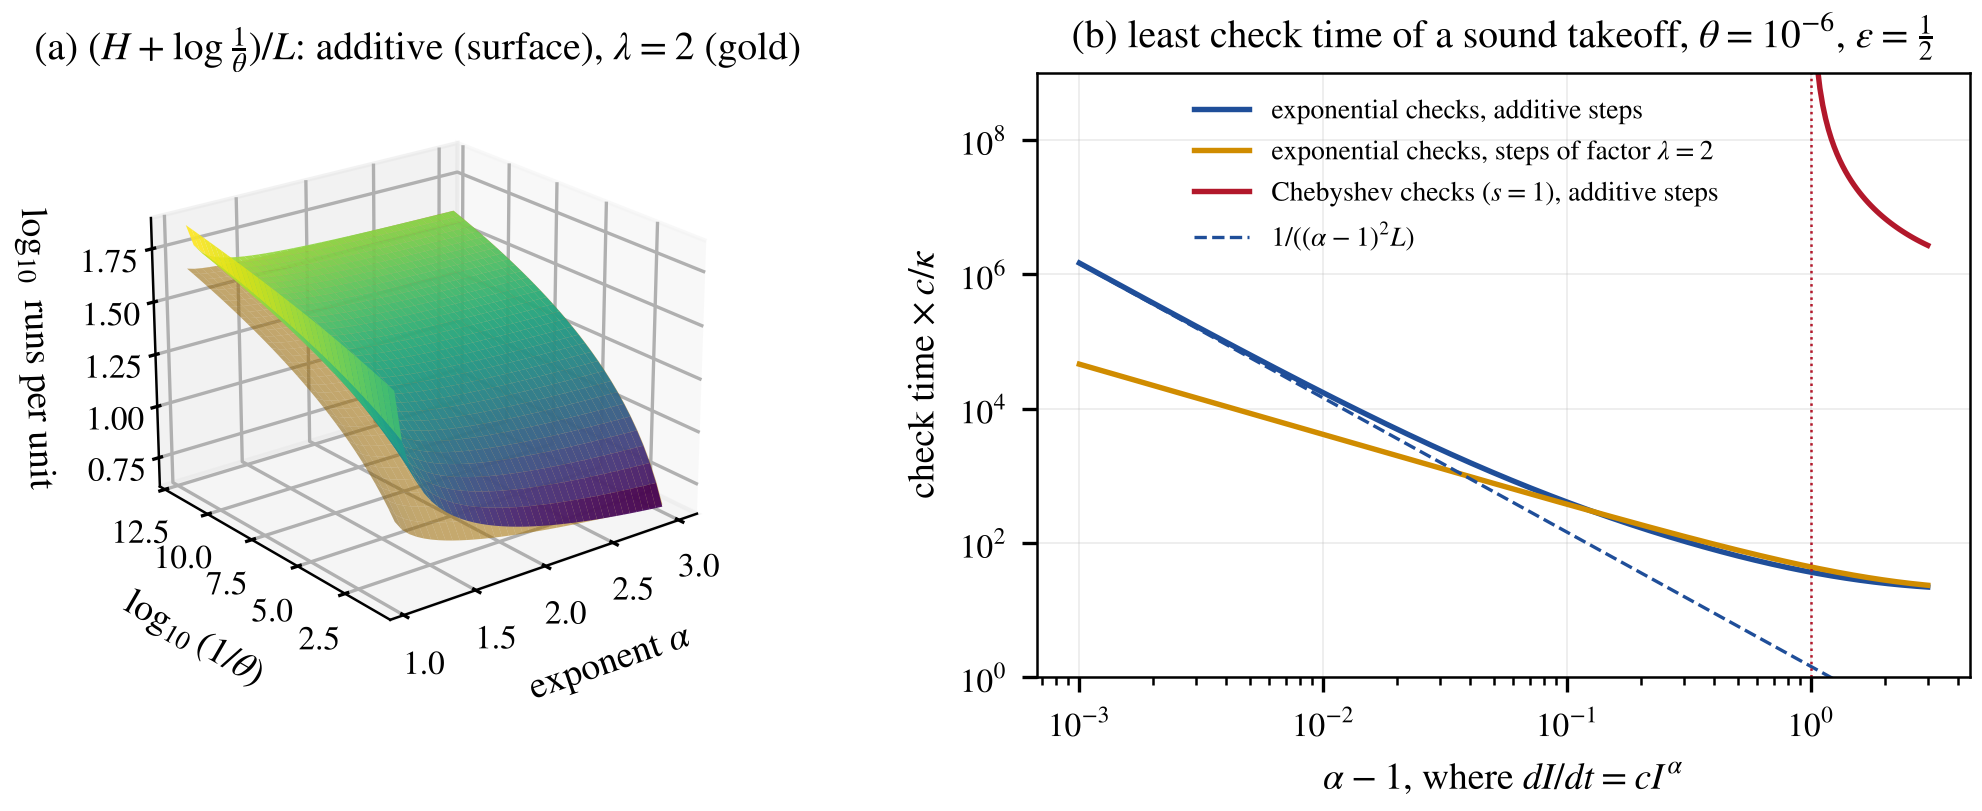
\includegraphics[width=0.98\textwidth]{figures/fig_takeoff}
\caption{Proposition~\ref{prop:osgood}, with $\eps=\frac12$. (a) The lower bound $(H+\log\frac1\theta)/L$ for the number of runs per unit of check cost, on a logarithmic scale, as a function of the growth exponent $\alpha$ and of $\log_{10}(1/\theta)$, for additive steps (coloured surface) and for doublings, $\lambda=2$ (gold surface). The additive surface rises like $1/(\alpha-1)$ as $\alpha\to1$, the multiplicative one like $\log\frac1{\alpha-1}$. (b) The lower bound for the least check time of a sound takeoff, in units of $\kappa/c$, at $\theta=10^{-6}$, against $\alpha-1$ on logarithmic axes: exponential checks with additive steps (blue), which approach $1/((\alpha-1)^{2}L)$ (dashed), exponential checks with doublings (gold), and Chebyshev checks with additive steps (red), which cost infinitely much for $\alpha\le2$ (dotted line).}
\label{fig:takeoff}
\end{figure*}

\subsection{What the growth exponent is, and what it is not}

The exponent $\alpha$ of Proposition~\ref{prop:osgood} is the elasticity of the speed of research with respect to the capability of the system that does it. It is not one of the exponents of the empirical scaling laws of language models. Kaplan and coauthors fitted the test loss of a language model trained with the optimal allocation of a compute budget $C$ to a power law $C^{-\alpha_{C}}$ with $\alpha_{C}\approx0.050$ \cite{KMH20}, and Hoffmann and coauthors fitted the loss as $E+A_{0}N^{-0.34}+B_{0}D^{-0.28}$ in the number $N$ of parameters and the number $D$ of training tokens \cite{HBM22}.\footnote{J.~Kaplan, S.~McCandlish, T.~Henighan, T.~B. Brown, B.~Chess, R.~Child, S.~Gray, A.~Radford, J.~Wu and D.~Amodei, \emph{Scaling laws for neural language models}, arXiv:2001.08361 (2020) \cite{KMH20}; J.~Hoffmann et~al., \emph{Training compute-optimal large language models}, arXiv:2203.15556 (2022) \cite{HBM22}. Both fits measure the cross-entropy loss on held-out text. The exponent $\alpha_{C}\approx0.050$ is that of the compute-efficient frontier in the first paper; the exponents $0.34$ and $0.28$, with fitted constants $E\approx1.69$, $A_{0}\approx406.4$ and $B_{0}\approx410.7$, are those of the parametric fit of the second. The letters $A_{0}$ and $B_{0}$ are renamed here to avoid a clash with the total cost $A$.} These laws relate loss to resources. To turn them into a value of $\alpha$ one needs two further maps, from loss to research ability and from research ability to the speed of the next improvement, and neither has been measured. Anbar Jafari, Ozcinar and Anbarjafari propose to estimate how fast improvement accelerates relative to its current level from series that engineers already record, which is an estimate of $\alpha$ \cite{AOA25}; the phase transitions and predictability limits of the first author with Singha Roy and Samal are a second approach to the same question \cite{BSS26}.

Ord observes that a singular growth path needs the generation time, the time around the loop of improvement, to tend to zero \cite{Ord26}. In the present model this is the condition $g_{n}\to0$, which a convergent $\sum g_{n}$ forces. Theorem~\ref{thm:E} adds a second clock: the time spent checking the $n$-th improvement must also tend to zero, and faster than the generation time can afford to, because the sum of $a_{n}\log(1/a_{n})$, and not only of $a_{n}$, must converge. Proposition~\ref{prop:osgood} shows that for power laws this second condition is free in kind and expensive in amount: every Osgood takeoff with $\alpha>1$ can be made sound with exponential checks, but near the threshold the checks take longer than the improvements by a factor that diverges as $1/(\alpha-1)$ when every unit of capability is checked. With checks that are only polynomially reliable, the threshold for a sound takeoff moves from $\alpha=1$ to $\alpha=1+s$, and between the two lies a range of singular takeoffs that cannot be made sound at any cost.

\begin{remark}[Errors of the generator]
Proposition~\ref{prop:osgood} prices the run in which every candidate is correct. If the $n$-th candidate is incorrect with probability in $[\rho_{\ast},\bar\rho]\subset(0,1)$ and incorrect candidates are regenerated, the proof of Theorem~\ref{thm:B}, with Proposition~\ref{prop:infinite} in place of Theorem~\ref{thm:A}, applies to the infinite chain: the lower bound holds with $\theta$ replaced by $\theta/\rho_{\ast}$, and the upper bound with $\theta$ replaced by $\theta(1-\bar\rho)/\bar\rho$ and the whole multiplied by $1/(1-\bar\rho)$. The orders in $\alpha-1$ of parts (ii) and (iii) do not change.
\end{remark}

\section{Formal proofs of hard problems}\label{sec:cases}

Several of the hardest problems of mathematics now have proofs that a machine has checked line by line, and three of these formal proofs were written with the help of artificial intelligence \cite{ZDC26,HBL26,OAI26}. They are the natural test of the theory: each is a long chain of steps, each step has a check, and each records which steps were hard. This section reads six of them in the language of Sections~\ref{sec:chains} and~\ref{sec:agents}, states what a BLLM adds and what it does not, and describes the package that implements the system.

\subsection{Six problems}

\begin{figure*}[t]
\centering
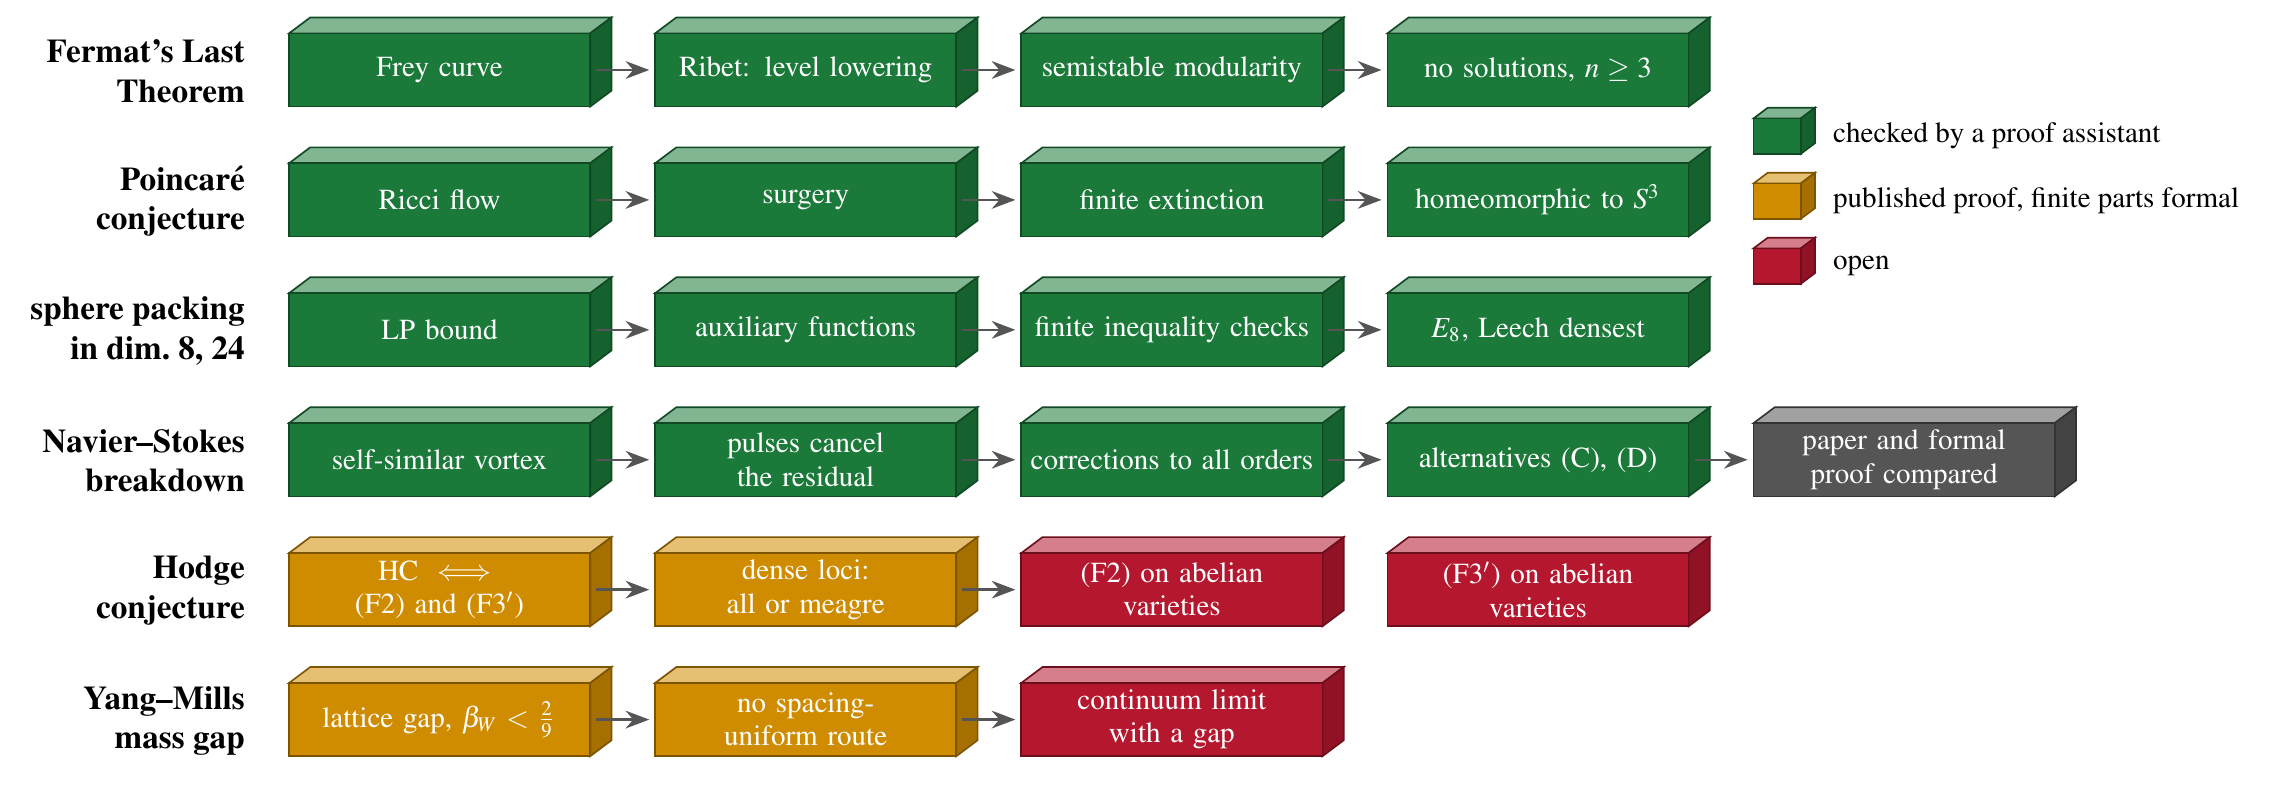
\includegraphics[width=0.98\textwidth]{figures/fig_cases}
\caption{The main steps of the six proofs of Table~\ref{tab:cases}. Green steps are checked by a proof assistant in an archived development, gold steps have published proofs that are not formalised, red steps are open, and grey marks the comparison of the Navier--Stokes paper with its formal proof \cite{BCH26}. The two Hodge statements (F2) and (F3$'$) are independent, and both are needed.}
\label{fig:cases}
\end{figure*}

Table~\ref{tab:cases} and Fig.~\ref{fig:cases} list the problems, the formal results and the steps that remain. Four are settled: Fermat's Last Theorem by Wiles and by Taylor and Wiles \cite{Wil95,TW95}; the Poincar\'e conjecture by Perelman, now formalised in Lean~4 with Mathlib following the account of Morgan and Tian \cite{ZDC26}; the sphere packing problem in dimensions $8$ and $24$ \cite{Via17,CKM17}, formalised by Hariharan, Birkbeck, Lee, Ma, Mehta, Poiroux and Viazovska and completed by Math, Inc. \cite{HBL26}; and finite-time breakdown of the three-dimensional Navier--Stokes equations with forcing, alternatives (C) and (D) of the official description of the Millennium problem, proved by OpenAI for every positive viscosity in a paper of 165 pages and in Lean \cite{OAI26}. Each formal development is archived with a record of an independent build \cite{ArcNS,ArcPC,ArcSP}. Two are open: the Hodge conjecture, which the first two authors reduced to two statements (F2) and (F3$'$) about abelian varieties \cite{BB26c}, and the existence of Yang--Mills theory with a mass gap, for which they proved a lattice mass gap for four-dimensional $\mathrm{SU}(2)$ up to the coupling $\beta_{W}=\frac29$, the limit of single-link Dobrushin arguments \cite{BB26d}.\footnote{D.~Bhattacharjee and U.~Bhattacharya, \emph{Dense algebraic loci of Hodge classes}, Hexagon preprint hexagon:2610.00315v1 (17 October 2026), with Lean~4 archive doi:10.5281/zenodo.23439578 \cite{BB26c}. The paper proves that the Hodge conjecture is equivalent to two statements about abelian varieties, that the locus on which either holds is dense in every family and is either the whole family or a meagre set, builds for each statement the object it needs next and proves at which step it stops. The second work, \emph{Lattice Yang--Mills theory: spacing-uniform obstructions, the mass gap up to the Dobrushin ceiling, and Lean certificate}, Zenodo (2026), doi:10.5281/zenodo.23449466 \cite{BB26d}, also proves that lattice inequalities uniform in the spacing cannot produce the continuum mass gap, and isolates the remaining step as one hypothesis on the ratio of the lattice gap to the spacing.}

\begin{table*}[t]
\caption{Six problems with machine-checked or published proofs, in the language of the moves of Section~\ref{ssec:moves}. ``Formal'' names the proof checker of the archived development; the last column names the moves on which the proof rests.}
\label{tab:cases}
\centering
\footnotesize
\setlength{\tabcolsep}{4pt}
\begin{tabular}{@{}p{0.13\textwidth}p{0.29\textwidth}p{0.08\textwidth}p{0.24\textwidth}p{0.17\textwidth}@{}}
\toprule
Problem & What is proved & Formal & What remains & Moves \\
\midrule
\rr Fermat's Last Theorem & \rr modularity of semistable elliptic curves, hence the theorem \cite{Wil95,TW95} & --- & \rr nothing; no formal proof in the archive & \rr bypass (Frey, Ribet), residual (Taylor--Wiles) \\
\rr Poincar\'e conjecture & \rr Hamilton--Perelman Ricci flow with surgery \cite{ZDC26} & Lean~4 & \rr nothing & \rr construction, residual (surgery) \\
\rr Sphere packing in dimensions 8, 24 & \rr $E_{8}$ and the Leech lattice are densest \cite{Via17,CKM17,HBL26} & Lean~4 & \rr nothing in dimensions 8, 24 & \rr construction, trivialization \\
\rr Navier--Stokes breakdown & \rr alternatives (C), (D) for every viscosity \cite{OAI26} & Lean~4 & \rr the correspondence of paper and formal proof \cite{BCH26} & \rr construction, residual, blow-up \\
\rr Hodge conjecture & \rr equivalence with (F2) and (F3$'$); dense loci \cite{BB26c} & \rr Lean~4, finite parts & \rr (F2), (F3$'$) & \rr bypass, strong then weak \\
\rr Yang--Mills mass gap & \rr lattice gap for $\beta_{W}<\frac29$; no spacing-uniform route \cite{BB26d} & \rr Lean~4, finite parts & \rr continuum limit with a gap & \rr construction, strong then weak, residual \\
\bottomrule
\end{tabular}
\end{table*}

The history of the problems contains the moves of Section~\ref{ssec:moves}. Wiles announced a proof in 1993 in which one step failed; the repair with Taylor replaced it by a different argument \cite{TW95}, a residual move on a single step of a long chain. The Navier--Stokes construction of \cite{OAI26} builds a self-similar vortex, cancels the singular part of its momentum residual by oscillatory pulses and corrects what is left to every order: construction, residual and blow-up in one argument. The sphere packing proofs reduce optimality to the existence of auxiliary functions whose inequalities are checked by finite computations, a trivialization. The Hodge reduction replaces the conjecture by statements on abelian varieties through known theorems, a bypass, and weakens one of them to (F3$'$), a step down the ladder of strong then weak.

\subsection{What a BLLM adds, and what it does not}

Three of the theorems of this paper speak directly to these proofs.

First, Theorem~\ref{thm:gating}. A formal development checks every step of the formal argument, not the steps of the paper it formalises. Bastounis, Circelli and Hansen argue that the Lean proof of \cite{OAI26} does not follow the argument of the paper, and that a faithful translation of a natural-language proof is not computable in general \cite{BCH26}. Whatever the outcome of that discussion, a natural-language argument whose only certificate is a formal proof of its final statement is checked at its outcome, and Theorem~\ref{thm:gating} shows that certification at the outcome is exponentially more expensive in the number of steps than certification step by step. A BLLM that keeps the paper and the formal proof aligned keeps a check at every step of both.

Second, Theorem~\ref{thm:cascade}. The developments above contain tens of thousands of formal lemmas, and the strong check, a full build, is expensive. A system that proposes most steps wrongly and filters them with cheap checks pays the build essentially only on its correct proposals, with a premium logarithmic in the ratio of costs; this is what makes very large numbers of machine proposals affordable without any loss of soundness.

Third, Theorem~\ref{thm:G} and Corollary~\ref{cor:onlinesing}. A system that keeps working on an open problem does not know how many steps it will take or what they will cost. The online law lets it run indefinitely with a guaranteed bound on the expected number of false acceptances over its whole life, at a cost within a double logarithm of the best schedule chosen with hindsight.

What the theorems do not give is the step that no proposer produces. The open entries of Table~\ref{tab:cases}, (F2), (F3$'$) and the continuum limit with a gap, are statements for which no proof has been proposed, by people or by machines. A BLLM cannot make them easier to prove: its guarantee is that whatever it keeps has been checked, at the least possible cost, and that its record of what failed, the residues, is complete. That record is the part of the work a later proposer, human or artificial, can build on.

\subsection{The package}\label{ssec:package}

The system of this paper is implemented as version~2 of the first author's package \texttt{eBLLM} \cite{Bha26c}, whose first version implemented the verifier-gated engine of \cite{Bha26a}. Version~2 adds the BLLM engine; it contains no source code of any language model, and the connectors call public interfaces with the user's own key. Its parts are the following.
\begin{enumerate}[label=(\alph*),leftmargin=1.8em,itemsep=1pt]
\item \emph{Schedules}: the entropy law and its ceiling schedule, Huffman schedules, the R\'enyi allocation, the online rule \eqref{eq:onlinerule}, the singularity test of Theorem~\ref{thm:E}, the amplified branching schedule, the proportional split of Theorem~\ref{thm:H} and the optimal cascade of Theorem~\ref{thm:cascade}.
\item \emph{Proposers}: connectors to hosted language models and to local models served through a compatible interface, and proposers that use no language model: enumerative program search, symbolic rewriting and Lean tactic search, with a deterministic proposer for reproducible runs.
\item \emph{Subagents}: one for each of the six moves of Section~\ref{ssec:moves}, under a coordinator that splits the budget by Theorem~\ref{thm:H}.
\item \emph{Checks}: the Lean kernel, exact evaluation, randomized polynomial identity tests \cite{Sch80,Zip79}, and arbitrary commands with checked output, arranged in cascades.
\item \emph{Memory}: every kept result is written as a Markdown note with links to the results it uses, so that the memory is a graph that can be opened as an Obsidian vault; the bypass move searches it.
\item \emph{Tasks}: the six problems of Table~\ref{tab:cases} as task files, each step labelled proved, partial or open from its published source, with the residues of every run.
\end{enumerate}
The package and the Lean development of this paper are archived with their own identifiers, given in the statement on data and code availability.

\section{What is proved and what is open}\label{sec:status}

\subsection{Proved}

Inside the model of Section~\ref{sec:model}, the paper determines the least cost of soundness. For finitely many candidates and exponential checks it is the entropy law, exact up to an additive term that is sharp (Theorem~\ref{thm:A}) and exact without remainder when the soundness is the reciprocal of an integer and the budget a power of it, where the optimal schedule is a Huffman code (Theorem~\ref{thm:C}). For checks of polynomial order the least cost is given in closed form by a R\'enyi entropy (Theorem~\ref{thm:D}), and for every cost function an infinite sequence of candidates admits a sound schedule of finite cost exactly when one series built from the concave conjugate of the cost converges (Theorem~\ref{thm:dual}). The same price, rescaled by the error rate of the generator, governs chains of improvements (Theorem~\ref{thm:B}), and checking only the outcome of a chain of $n$ steps is exponentially more expensive than checking every step (Theorem~\ref{thm:gating}). An infinite chain reaches a singularity soundly exactly when the costs of its checks have finite entropy in addition to a finite sum, which fails for a nonempty range of cost laws (Theorem~\ref{thm:E}, Corollary~\ref{cor:gap}); a branching takeoff with a fixed false acceptance rate keeps infinitely many errors on survival, and a sound one needs a number of runs that grows linearly with the generation (Theorem~\ref{thm:F}). In the Osgood model of growth every singular takeoff can be made sound with exponential checks, at a price of order $1/(\alpha-1)^{2}$ near the critical exponent, while polynomial checks move the threshold of a sound takeoff from $\alpha=1$ to $\alpha=1+s$ (Proposition~\ref{prop:osgood}).

The finite inequalities behind these statements are proved in Lean~4 (Appendix~\ref{app:checks}). The probabilistic limit theorems, Wald's identity, the Kesten--Stigum theorem, L\'evy's conditional Borel--Cantelli lemma and the extinction theorem of Galton--Watson processes, are classical and are proved or cited in Appendix~\ref{app:derivations}; the asymptotics of $\zeta$ near $1$ are proved in the text.

\subsection{Open}

Three questions are left open, and each is a precise mathematical question.

\emph{Adaptive protocols.} Remark~\ref{rem:adaptive} shows that a protocol which looks at the outcomes of the checks can avoid the entropy term by halting at the first rejection, at the price of losing the correct work after it. Let a protocol be \emph{conservative} if, in every world, it keeps every correct candidate with probability one. Is the least worst-case expected cost of a conservative $\theta$-sound protocol equal to $\Vs(\theta)$ up to an additive $O(A)$? An adaptive protocol may let the number of runs of later checks depend on the results of earlier ones; since a correct candidate never fails, a conservative protocol learns nothing from the runs of a candidate that passes, and the question is whether the information it gains from rejections can be converted into a saving that is not $O(A)$.

\emph{Two-sided checks.} For checks that err on both sides Proposition~\ref{prop:twosided} gives the entropy law with the rate $D=\mathrm{KL}(\mathrm{Ber}(\frac12)\,\|\,\mathrm{Ber}(q))$ in the upper bound and $\log(1/q)$ in the lower bound. The exact rate of a sequential test with two error probabilities is Wald's \cite{Wal45}, and the question is whether the optimal schedule for many two-sided checks attains the entropy law with the Chernoff rate of the pair of hypotheses, in both directions.

\emph{Correlated runs.} The model assumes that the runs of a check are independent. A real verifier, a learned reward model or a test suite run on the same machine, has correlated errors, and repeated runs of a deterministic check gain nothing. The entropy law holds for every family of checks whose false acceptance probability after $r$ runs is at most $\eps^{r}$, whatever the mechanism; the open question is which checks used in practice have this property, with which $\eps$, and what replaces the law for those that do not.

\subsection{What is not claimed}

The paper does not claim that any existing system is sound or that an intelligence explosion will or will not occur. Its theorems are statements about a model with independent runs, perfect completeness and schedules fixed in advance, and their value for a real system depends on how well that system satisfies them. What is claimed is that inside the model the cost of soundness is computable, that it is an entropy, and that it divides the singular processes into those that can be made sound and those that cannot.


\appendix
\section{Classical facts used in the proofs}\label{app:derivations}

This appendix proves, or states with a precise reference, the classical results that the main text uses. Nothing here is new; the proofs are given so that the paper can be read without the references.

\subsection{Kraft's inequality and McMillan's theorem}\label{app:kraft}

Fix an integer $D\ge2$. A word of length $\ell$ over the alphabet $\{0,\dots,D-1\}$ is identified with the interval
\[
J(w)=\Bigl[\,\sum_{j=1}^{\ell}w_{j}D^{-j},\ \sum_{j=1}^{\ell}w_{j}D^{-j}+D^{-\ell}\Bigr)\subset[0,1),
\]
the set of reals in $[0,1)$ whose $D$-ary expansion, taken without a tail of digits $D-1$, begins with $w$. Two intervals $J(w)$ and $J(w')$ meet if and only if one of the words is a prefix of the other: if $w$ is a prefix of $w'$ then $J(w')\subset J(w)$, and otherwise the two expansions differ at some position not beyond the shorter length, so no real begins with both.

\begin{proposition}[Kraft]
Lengths $\ell_{1},\dots,\ell_{n}\in\NN$ are those of a $D$-ary prefix code if and only if $\sum_{i}D^{-\ell_{i}}\le1$.
\end{proposition}

\begin{proof}
If the words form a prefix code, the intervals $J(w_{i})$ are disjoint subsets of $[0,1)$ of lengths $D^{-\ell_{i}}$, so their lengths add up to at most $1$. Conversely, order the lengths so that $\ell_{1}\le\dots\le\ell_{n}$ and put $c_{i}=\sum_{j<i}D^{-\ell_{j}}$. Each $D^{-\ell_{j}}$ with $j<i$ is a multiple of $D^{-\ell_{i}}$, so $c_{i}D^{\ell_{i}}$ is an integer, and $c_{i}+D^{-\ell_{i}}\le\sum_{j}D^{-\ell_{j}}\le1$, so $0\le c_{i}D^{\ell_{i}}\le D^{\ell_{i}}-1$. Let $w_{i}$ be the expansion of this integer in base $D$ with exactly $\ell_{i}$ digits. Then $J(w_{i})=[c_{i},c_{i+1})$, these intervals are disjoint, and the words form a prefix code.
\end{proof}

\begin{proposition}[McMillan]
If a code with lengths $\ell_{1},\dots,\ell_{n}$ is uniquely decodable, that is, distinct finite sequences of codewords have distinct concatenations, then $\sum_{i}D^{-\ell_{i}}\le1$.
\end{proposition}

\begin{proof}
Let $M=\max_{i}\ell_{i}$ and $k\ge1$. Expanding the $k$-th power,
\[
\Bigl(\sum_{i}D^{-\ell_{i}}\Bigr)^{k}=\sum_{i_{1},\dots,i_{k}}D^{-(\ell_{i_{1}}+\dots+\ell_{i_{k}})}=\sum_{m=k}^{kM}N_{m}D^{-m},
\]
where $N_{m}$ is the number of $k$-tuples of codewords whose concatenation has length $m$. By unique decodability these concatenations are distinct words of length $m$, so $N_{m}\le D^{m}$ and the sum is at most $kM$. Hence $\sum_{i}D^{-\ell_{i}}\le(kM)^{1/k}$ for every $k$, and $(kM)^{1/k}\to1$.
\end{proof}

\subsection{Huffman's algorithm}\label{app:huffman}

Let $p_{1}\ge\dots\ge p_{n}\ge0$ with $\sum p_{i}=1$, and let $L_{D}(p)$ be the least value of $\sum_{i}p_{i}\ell_{i}$ over $\ell\in\NN^{n}$ with $\sum_{i}D^{-\ell_{i}}\le1$. The minimum exists: let $c_{0}$ be the cost of the code in which every word has length $\lceil\log_{D}n\rceil$; a vector of cost at most $c_{0}$ has $\ell_{i}\le c_{0}/p_{i}$ for every $i$ with $p_{i}>0$, and the cost does not depend on the other lengths, so it takes only finitely many values at most $c_{0}$. Huffman's algorithm \cite{Huf52} is the following recursion. If $n=1$ the code is the empty word. Otherwise add zero weights until $n\equiv1\pmod{D-1}$, merge the $D$ smallest weights into one symbol whose weight is their sum, solve the smaller problem, and give the $D$ merged symbols the codeword of their merger followed by each of the $D$ letters.

\begin{proposition}[Huffman]
The algorithm returns a prefix code of expected length $L_{D}(p)$.
\end{proposition}

\begin{proof}
\emph{Step 1: padding is free.} Adding a symbol of weight $0$ cannot lower the optimum, since removing a codeword from a code keeps Kraft's inequality and the cost. It does not raise it either, by the following argument. Let $\ell$ be optimal for $p$ with $n\not\equiv1\pmod{D-1}$, and let $M=\max\ell_{i}$. Since $D^{M-\ell_{i}}\equiv1\pmod{D-1}$, the integer $\sum_{i}D^{M-\ell_{i}}$ is congruent to $n$, and $D^{M}$ to $1$, modulo $D-1$; so $\sum_{i}D^{-\ell_{i}}<1$, the difference being a positive multiple of $D^{-M}$. Zero weights at lengths $M+1,\dots,M+k$ add $\sum_{j=1}^{k}D^{-M-j}<D^{-M}$ to the Kraft sum and nothing to the cost. So we may assume $n\equiv1\pmod{D-1}$.

\emph{Step 2: an optimal code with equality.} Among the optimal $\ell$ choose one with $\sum_{i}\ell_{i}$ least, and let $M=\max\ell_{i}$; if $M=0$ then $n=1$. By the congruence of Step~1, now with $n\equiv1$, the deficit $\Delta=1-\sum_{i}D^{-\ell_{i}}$ satisfies $\Delta D^{M}\equiv0\pmod{D-1}$. If $\Delta>0$, then $\Delta\ge(D-1)D^{-M}$, and shortening one word of length $M$ by one letter adds $(D-1)D^{-M}$ to the Kraft sum, keeps it at most $1$, does not raise the cost and lowers $\sum\ell_{i}$, a contradiction. So $\sum_{i}D^{-\ell_{i}}=1$.

\emph{Step 3: the smallest weights are deepest.} If $p_{i}>p_{j}$ and $\ell_{i}>\ell_{j}$, exchanging the two lengths lowers the cost by $(p_{i}-p_{j})(\ell_{i}-\ell_{j})>0$; so in an optimal code $p_{i}>p_{j}$ implies $\ell_{i}\le\ell_{j}$, and among equal weights the lengths may be permuted freely. Multiplying the equality of Step~2 by $D^{M}$, every word shorter than $M$ contributes a multiple of $D$, so the number of words of length $M$ is a positive multiple of $D$, hence at least $D$. By the exchange we may assume that the $D$ smallest weights $p_{n-D+1},\dots,p_{n}$ have length $M$.

\emph{Step 4: the recursion.} Let $p'$ be the vector of $n-D+1\equiv1\pmod{D-1}$ weights obtained by merging the $D$ smallest into $\sigma=p_{n-D+1}+\dots+p_{n}$. The lengths of Step~3, with the merged symbol at length $M-1$, satisfy Kraft's inequality for $p'$, since $D\cdot D^{-M}=D^{-(M-1)}$, and have cost $\sum_{i}p_{i}\ell_{i}-\sigma$; so $L_{D}(p')\le L_{D}(p)-\sigma$. Conversely, a code for $p'$ in which the merged symbol has length $\ell'$ gives a code for $p$ by giving the $D$ merged symbols length $\ell'+1$, with the same Kraft sum and cost increased by $\sigma$; so $L_{D}(p)\le L_{D}(p')+\sigma$. Hence $L_{D}(p)=L_{D}(p')+\sigma$, which is the recursion of the algorithm, and induction on $n$ concludes.
\end{proof}

\subsection{Wald's identity and the geometric number of retries}\label{app:wald}

Let $c_{1},c_{2},\dots$ be independent and identically distributed costs of successive candidates, with finite mean, and let $K$ be the index of the first candidate kept, where whether candidate $j$ is kept depends only on candidate $j$, with probability $s>0$. Then $K$ is geometric, $\EE K=1/s$, and $\EE\sum_{j\le K}c_{j}=\EE K\cdot\EE c_{1}$ \cite{Wal45}. Indeed $\{K\ge j\}$ is determined by the candidates $1,\dots,j-1$ and is therefore independent of $c_{j}$, so by monotone convergence $\EE\sum_{j\le K}c_{j}=\sum_{j}\EE[c_{j}]\PR(K\ge j)=\EE c_{1}\sum_{j}\PR(K\ge j)=\EE c_{1}\,\EE K$. This is the identity used in Lemma~\ref{lem:onestep}.

\subsection{Products and the Borel--Cantelli lemmas}\label{app:bc}

Let $0\le\pi_{n}<1$. If $\sum\pi_{n}<\infty$ then $\prod_{n}(1-\pi_{n})>0$: for $n$ large $\pi_{n}\le\frac12$, and $\log(1-x)\ge-2x$ on $[0,\frac12]$, so the logarithm of the tail of the product is at least $-2\sum_{n\ge N}\pi_{n}>-\infty$, and the first factors are positive. If $\sum\pi_{n}=\infty$ then $\prod_{n\ge N}(1-\pi_{n})\le\exp(-\sum_{n\ge N}\pi_{n})=0$ for every $N$. For independent events $E_{n}$ with $\PR(E_{n})=\pi_{n}$ the second statement is the second Borel--Cantelli lemma, since $\PR(\text{no }E_{n}\text{ with }n\ge N)=\prod_{n\ge N}(1-\pi_{n})=0$ for every $N$; the first Borel--Cantelli lemma, that $\sum\PR(E_{n})<\infty$ implies that only finitely many $E_{n}$ occur, needs no independence, because $\EE\sum\ind_{E_{n}}=\sum\PR(E_{n})<\infty$ \cite{Bor09,Dur19}.

\subsection{L\'evy's conditional Borel--Cantelli lemma}\label{app:levy}

Let $(\mathcal F_{k})$ be a filtration, $B_{k}\in\mathcal F_{k}$ and $p_{k}=\PR(B_{k}\mid\mathcal F_{k-1})$. Then, up to a null set, $\{B_{k}\text{ infinitely often}\}=\{\sum_{k}p_{k}=\infty\}$ \cite[Section~4.3]{Dur19}.

\begin{proof}
$M_{n}=\sum_{k\le n}(\ind_{B_{k}}-p_{k})$ is a martingale with increments bounded by $1$. For such a martingale, almost surely either $M_{n}$ converges to a finite limit or $\limsup M_{n}=+\infty$ and $\liminf M_{n}=-\infty$ \cite[Section~4.3]{Dur19}. Write $\sum_{k\le n}\ind_{B_{k}}=M_{n}+\sum_{k\le n}p_{k}$; the left side is nonnegative and nondecreasing. On $\{\sum p_{k}<\infty\}$, $\liminf M_{n}=-\infty$ would make the left side negative, so $M_{n}$ converges and $\sum\ind_{B_{k}}<\infty$. On $\{\sum p_{k}=\infty\}$, if $\sum\ind_{B_{k}}<\infty$ then $M_{n}\to-\infty$, which is neither alternative; so $\sum\ind_{B_{k}}=\infty$.
\end{proof}

\subsection{Cauchy's condensation test}\label{app:condensation}

If $b_{n}\ge0$ is nonincreasing for $n\ge n_{0}$, then $\sum_{n}b_{n}<\infty$ if and only if $\sum_{k}2^{k}b_{2^{k}}<\infty$. Indeed, for $2^{k}\ge n_{0}$ the block $2^{k}\le n<2^{k+1}$ has $2^{k}$ terms, each between $b_{2^{k+1}}$ and $b_{2^{k}}$, so its sum lies between $\frac12\,2^{k+1}b_{2^{k+1}}$ and $2^{k}b_{2^{k}}$. For $b_{n}=1/(n\log^{c}n)$, which is eventually nonincreasing for every real $c$, the condensed terms are $(k\log2)^{-c}$, and their series converges if and only if $c>1$.

\subsection{Sums and integrals of unimodal functions}\label{app:zeta}

Let $f\ge0$ be integrable on $[1,\infty)$, nondecreasing on $[1,x_{0}]$ and nonincreasing on $[x_{0},\infty)$, with maximum $M_{f}=f(x_{0})$. Then
\[
\Bigl|\sum_{n\ge1}f(n)-\int_{1}^{\infty}f(x)\,dx\Bigr|\le M_{f}.
\]
Let $N=\lfloor x_{0}\rfloor$. For $1\le n\le N-1$, $f$ is nondecreasing on $[n,n+1]$, so $f(n)\le\int_{n}^{n+1}f\le f(n+1)$; for $n\ge N+1$, $f$ is nonincreasing on $[n,n+1]$, so $f(n+1)\le\int_{n}^{n+1}f\le f(n)$. Summing,
\[
\begin{aligned}
\sum_{n\ge1}f(n)&\le\int_{1}^{N}f+f(N)+f(N+1)+\int_{N+1}^{\infty}f,\\
\sum_{n\ge1}f(n)&\ge f(1)+\int_{1}^{N}f+\int_{N+1}^{\infty}f .
\end{aligned}
\]
On $[N,N+1]$ the function is at least $\min(f(N),f(N+1))$, because it rises and then falls there; so $\int_{N}^{N+1}f\ge\min(f(N),f(N+1))$, and the first inequality gives $\sum f(n)\le\int_{1}^{\infty}f+\max(f(N),f(N+1))$. The second gives $\sum f(n)\ge\int_{1}^{\infty}f-\int_{N}^{N+1}f\ge\int_{1}^{\infty}f-M_{f}$. For $f(x)=x^{-p}\log x$ with $p>1$ one has $x_{0}=e^{1/p}$, $M_{f}=1/(pe)$ and $\int_{1}^{\infty}f=1/(p-1)^{2}$, which is the estimate used in Proposition~\ref{prop:powerlaw}; the same argument, with $x_{0}=1$, gives $1/(p-1)\le\zeta(p)\le1+1/(p-1)$.

\subsection{Extinction of a Galton--Watson process}\label{app:gw}

Let $N\ge0$ be an integer random variable with $f(z)=\EE z^{N}$, mean $m=f'(1^{-})\in[0,\infty]$ and $\PR(N=1)<1$, and let $(Z_{k})$ be the Galton--Watson process with $Z_{0}=1$ and offspring law $N$. Then the extinction probability $e=\PR(Z_{k}=0\text{ for some }k)$ is the least root of $f(z)=z$ in $[0,1]$, and $e=1$ if and only if $m\le1$ \cite{AN72,WG75}.

\begin{proof}
Conditioning on the first generation, the generating function of $Z_{k}$ is the $k$-fold composition $f_{k}=f\circ\dots\circ f$, so $\PR(Z_{k}=0)=f_{k}(0)$. These numbers increase with $k$ to $e$, and $f(e)=e$ by continuity of $f$ on $[0,1]$. If $z^{\ast}\in[0,1]$ is a root, then $f_{k}(0)\le f_{k}(z^{\ast})=z^{\ast}$ because $f$ is nondecreasing, so $e\le z^{\ast}$: $e$ is the least root. If $\PR(N\ge2)=0$, then $f(z)=\PR(N=0)+\PR(N=1)z$ with $m=\PR(N=1)<1$, and $f(z)>z$ on $[0,1)$, so $e=1$. Otherwise $f'$ is strictly increasing on $[0,1)$. If $m\le1$, then $f'(z)<1$ on $[0,1)$, so $f(z)-z$ is strictly decreasing there with limit $0$ at $1$, hence positive, and the only root is $1$. If $m>1$, then $f(z)<z$ for $z<1$ close to $1$, while $f(0)\ge0$, so there is a root in $[0,1)$, and $e<1$.
\end{proof}

The theorem of Kesten and Stigum \cite{KS66}, used in the proof of Theorem~\ref{thm:F}, is not proved here: if $1<m<\infty$, the martingale $Z_{k}/m^{k}$ converges almost surely to a limit $W$, and $W>0$ almost surely on survival if and only if $\EE N\log N<\infty$; the proof is in \cite[Chapter~I]{AN72}.

\section{Formal proofs and numerical checks}\label{app:checks}

\subsection{The Lean development}

The finite inequalities of the paper are proved in Lean~4 with Mathlib, in eleven files and thirty-nine theorems, listed in Table~\ref{tab:lean}. Every theorem depends only on the three standard axioms of Lean, propositional extensionality, the axiom of choice and the soundness of quotients; the command \texttt{\#print axioms} is run on each of them, and no theorem uses \texttt{sorry}. The statements are over the real numbers, with finite sums indexed by a \texttt{Finset} and infinite ones expressed by \texttt{Summable}; in them $\sigma$ is the polynomial order written $s$ in the text, and $(1/D)^{r}$ is $\eps^{r}$ with $\eps=1/D$.

The formal statements cover the deterministic content of the main theorems: Gibbs' inequality in the form used for the entropy law, the lower bound and the two properties of the ceiling schedule (Theorem~\ref{thm:A}), the correspondence between schedules and Kraft vectors and the shifted cost (Theorem~\ref{thm:C}), H\"older's lower bound and the optimal allocation of the R\'enyi law (Theorem~\ref{thm:D}) with the summability criterion for polynomial checks, both halves of the duality criterion (Theorem~\ref{thm:dual}), the inequalities for clean runs and random schedules (Propositions~\ref{prop:clean} and~\ref{prop:random}), the precision and cost identities of the gating theorem (Theorem~\ref{thm:gating}), the summability criterion for sound singular chains with both directions (Theorem~\ref{thm:E}(iii)), the two Borel--Cantelli statements for false acceptances (Theorem~\ref{thm:E}(i)), and the divergence and amplification statements of the branching theorem (Theorem~\ref{thm:F}). The limit theorems of probability (Wald's identity, the extinction theorem, the Kesten--Stigum theorem and L\'evy's lemma), the asymptotics of $\zeta$ and of the entropies in Propositions~\ref{prop:powerlaw} and~\ref{prop:osgood}, and the estimates of Proposition~\ref{prop:twosided} are proved in the text and are not formalised.

\begin{table*}[t]
\caption{The thirty-nine theorems of the Lean development, by file. The third column gives the statement in the notation of the paper and the fourth the result in which it is used. Sums over $i$ are finite; sums over $n$ or $k$ are infinite and ``$\sum<\infty$'' means summability.}
\label{tab:lean}
\centering
\footnotesize
\begin{tabular}{@{}l l p{0.53\textwidth} l@{}}
\toprule
File & Theorem & Statement & Used in \\
\midrule
\texttt{Basic} & \lean{gibbs\_term} & $x\log\frac1x\le x\log\frac1y+y-x$ for $x,y>0$ & Lemma~\ref{lem:gibbs} \\
 & \lean{entropy\_term} & $a\log\frac Aa+a\log\frac1\theta\le a\log\frac1b+\frac{Ab}\theta-a$ & Lemma~\ref{lem:entropyterm} \\
 & \lean{log\_inv\_pow} & $\log(1/\eps^{r})=r\log(1/\eps)$ & Theorem~\ref{thm:A} \\
 & \lean{log\_inv\_pos} & $\log(1/\eps)>0$ for $0<\eps<1$ & Theorem~\ref{thm:A} \\
\texttt{EntropyLaw} & \lean{entropy\_lower} & $\sum\beta_{i}\le\theta\Rightarrow\sum a_{i}\log\frac A{a_{i}}+A\log\frac1\theta\le\sum a_{i}\log\frac1{\beta_{i}}$ & Proposition~\ref{prop:entropyineq} \\
 & \lean{verification\_lower} & $\sum\eps^{r_{i}}\le\theta\Rightarrow\frac AL(H+\log\frac1\theta)\le\sum a_{i}r_{i}$ & Theorem~\ref{thm:A} \\
 & \lean{ceilSchedule\_sound} & the ceiling schedule has $\sum\eps^{r_{i}}\le\theta$ & Theorem~\ref{thm:A} \\
 & \lean{ceilSchedule\_cost} & the ceiling schedule costs at most $\frac AL(H+\log\frac1\theta)+A$ for $\theta\le1$ & Theorem~\ref{thm:A} \\
\texttt{Kraft} & \lean{kraft\_of\_schedule} & $\sum D^{-r_{i}}\le D^{-k}\Rightarrow r_{i}\ge k$ and $\sum D^{-(r_{i}-k)}\le1$ & Lemma~\ref{lem:kraftsound}(i) \\
 & \lean{schedule\_of\_kraft} & $\sum D^{-\ell_{i}}\le1\Rightarrow\sum D^{-(\ell_{i}+k)}\le D^{-k}$ & Lemma~\ref{lem:kraftsound}(ii) \\
 & \lean{shifted\_cost} & $\sum a_{i}(\ell_{i}+k)=kA+\sum a_{i}\ell_{i}$ & Lemma~\ref{lem:kraftsound}(iii) \\
\texttt{Renyi} & \lean{renyi\_lower} & $\sum\delta_{i}\le\theta\Rightarrow(\sum a_{i}^{1/(1+s)})^{1+s}\le\theta^{s}\sum a_{i}\delta_{i}^{-s}$ & Theorem~\ref{thm:D} \\
 & \lean{renyi\_attain} & $\delta_{i}=\theta a_{i}^{1/(1+s)}/S$ has $\sum\delta_{i}=\theta$ and cost $\theta^{-s}S^{1+s}$ & Theorem~\ref{thm:D} \\
 & \lean{poly\_schedule\_iff} & a positive $\delta$ with $\sum\delta_{n}<\infty$, $\sum a_{n}\delta_{n}^{-s}<\infty$ exists $\iff\sum a_{n}^{1/(1+s)}<\infty$ & Corollary~\ref{cor:dualcases}(ii) \\
\texttt{Duality} & \lean{dualCost\_nonneg} & $\psi(u)\ge0$ for $u\ge0$ & Theorem~\ref{thm:dual} \\
 & \lean{dualCost\_le} & $\psi(u)\le\kappa(\delta)+u\delta$ for $\delta\in(0,1]$ & Theorem~\ref{thm:dual} \\
 & \lean{dual\_summable\_of\_schedule} & a sound allocation of finite cost gives $\sum a_{n}\psi(\lambda/a_{n})<\infty$ for every $\lambda>0$ & Theorem~\ref{thm:dual} \\
 & \lean{schedule\_of\_dual\_summable} & $\sum a_{n}\psi(\lambda/a_{n})<\infty$ for one $\lambda>0$ gives a sound allocation of finite cost & Theorem~\ref{thm:dual} \\
\texttt{Clean} & \lean{clean\_le\_exp} & $\prod(1-q_{i})\le e^{-\sum q_{i}}$ for $q_{i}\le1$ & Proposition~\ref{prop:clean} \\
 & \lean{clean\_ge} & $1-\sum q_{i}\le\prod(1-q_{i})$ for $0\le q_{i}\le1$ & Proposition~\ref{prop:clean} \\
 & \lean{clean\_budget} & $\prod(1-q_{i})\ge1-\theta\Rightarrow\sum q_{i}\le\log\frac1{1-\theta}$ & Proposition~\ref{prop:clean} \\
\texttt{Adaptive} & \lean{jensen\_repetition} & $\eps^{\sum w_{j}r_{j}}\le\sum w_{j}\eps^{r_{j}}$ for weights $w$ & Proposition~\ref{prop:random} \\
 & \lean{randomised\_budget} & a random schedule within budget in mean has its mean within budget & Proposition~\ref{prop:random} \\
\texttt{Gating} & \lean{step\_precision} & $\frac{(1-\rho)(1-\eta)}{(1-\rho)(1-\eta)+\rho\delta}=\frac1{1+x}$ & Theorem~\ref{thm:gating}(i) \\
 & \lean{precision\_bounds} & $e^{-\sum x_{i}}\le\prod(1+x_{i})^{-1}\le e^{-\sum x_{i}/(1+x_{i})}$ & Theorem~\ref{thm:gating}(i) \\
 & \lean{outcome\_precision} & $\frac{c(1-\eta_{o})}{c(1-\eta_{o})+(1-c)\delta_{o}}=\bigl(1+\frac{(1-c)\delta_{o}}{c(1-\eta_{o})}\bigr)^{-1}$ & Theorem~\ref{thm:gating}(ii) \\
 & \lean{separation} & cost ratio $(1-\rho)^{-n}$ and $1+n\rho\le(1-\rho)^{-n}$ & Theorem~\ref{thm:gating}(iii) \\
\texttt{Singularity} & \lean{entropy\_summable\_of\_schedule} & $\sum\eps^{r_{n}}<\infty$, $\sum a_{n}r_{n}<\infty$, $a_{n}\le1\Rightarrow\sum a_{n}\log\frac1{a_{n}}<\infty$ & Theorem~\ref{thm:E}(iii) \\
 & \lean{costSchedule\_pow\_le} & $r_{n}=\lceil\log(1/a_{n})/L\rceil$ has $\eps^{r_{n}}\le a_{n}$ & Proposition~\ref{prop:integer} \\
 & \lean{schedule\_of\_entropy\_summable} & $\sum a_{n}<\infty$, $\sum a_{n}\log\frac1{a_{n}}<\infty$ make that schedule sound and of finite cost & Theorem~\ref{thm:E}(iii) \\
 & \lean{sound\_schedule\_iff} & for $\sum a_{n}<\infty$, $a_{n}\le1$: a sound schedule of finite cost exists $\iff\sum a_{n}\log\frac1{a_{n}}<\infty$ & Proposition~\ref{prop:integer} \\
 & \lean{shift\_schedule} & $\eps^{r_{n}+k}=\eps^{k}\eps^{r_{n}}$ & Theorem~\ref{thm:E}(iii) \\
\texttt{Soundness} & \lean{false\_accepts\_finite} & $\PR(E_{n})\le Cq_{n}$, $\sum q_{n}<\infty\Rightarrow\PR(E_{n}\text{ i.o.})=0$ & Theorem~\ref{thm:E}(i) \\
 & \lean{false\_accepts\_infinite} & independent $E_{n}$, $\PR(E_{n})\ge bq_{n}$, $b>0$, $\sum q_{n}=\infty\Rightarrow\PR(E_{n}\text{ i.o.})=1$ & Theorem~\ref{thm:E}(i) \\
 & \lean{any\_false\_accept\_le} & $\PR(\bigcup E_{n})\le C\sum q_{n}$ & Theorem~\ref{thm:E}(i) \\
\texttt{Branching} & \lean{contamination\_diverges} & $\sum m^{k}\delta=\infty$ for $m\ge1$, $\delta>0$ & Theorem~\ref{thm:F} \\
 & \lean{amplified\_term} & $k\log(2m)\le r_{k}L\Rightarrow m^{k}\eps^{r_{k}}\le2^{-k}$ & Theorem~\ref{thm:F} \\
 & \lean{amplified\_summable} & under the same hypothesis $\sum m^{k}\eps^{r_{k}}<\infty$ & Theorem~\ref{thm:F} \\
 & \lean{amplified\_schedule\_ok} & $r_{k}=\lceil k\log(2m)/L\rceil$ satisfies that hypothesis & Theorem~\ref{thm:F} \\
\bottomrule
\end{tabular}
\end{table*}

\subsection{Numerical checks}

Independent programs test the closed forms of the paper against exhaustive searches, exact optima and simulation, on instances drawn with fixed seeds. They are listed in Table~\ref{tab:checks}; the shell script that runs them also builds the Lean development and prints the axioms of every theorem, and it reports $33{,}505$ checks with no failure. The checks are not part of any proof. They guard against errors in the statements: a wrong constant, a reversed inequality or a misprinted formula would make one of them fail. The numerical values quoted in the text, in Tables~\ref{tab:huffman} and~\ref{tab:gw} and in the figures are produced by the same programs.

\begin{table}[!htb]
\caption{The numerical checks.}
\label{tab:checks}
\centering
\footnotesize
\begin{tabular}{@{}l >{\raggedright\arraybackslash}p{0.56\columnwidth} r@{}}
\toprule
Language & What is checked & Checks \\
\midrule
Python & Theorems~\ref{thm:A}, \ref{thm:C}: bounds and Huffman cost against exact optima & 649 \\
Python & Theorem~\ref{thm:gating}: costs and precisions against simulation & 533 \\
Python & Theorems~\ref{thm:D}, \ref{thm:dual}: R\'enyi optimum, dual costs & 20{,}850 \\
Python & Theorem~\ref{thm:E}, Propositions~\ref{prop:powerlaw}, \ref{prop:osgood} & 241 \\
Python & Theorem~\ref{thm:F}: takeoff, kept errors, amplified checks & 2{,}432 \\
C & Theorem~\ref{thm:C}: exhaustive search over schedules & 800 \\
C\texttt{++} & Theorems~\ref{thm:D}, \ref{thm:gating} at random feasible points & 8{,}000 \\
\midrule
 & total & 33{,}505 \\
\bottomrule
\end{tabular}
\end{table}


\section*{Acknowledgements}
The paper builds on Claude Shannon's coding theorem, David Huffman's algorithm, the inequalities of Leon Kraft and Brockway McMillan, Alfr\'ed R\'enyi's entropies and L.~L. Campbell's coding theorem for them, the branching processes of Watson, Galton, Otter, Kesten and Stigum, and the Borel--Cantelli lemmas. The recent analyses of verifiers by Jia, Rakhlin and Xie, by Rohatgi and coauthors and by Balcan and coauthors, and Toby Ord's study of the dynamics of intelligence explosions, fixed the questions it answers. We thank the developers of Lean and Mathlib.

\section*{Data and code availability}
The \LaTeX{} source of the paper, the Lean~4 development of Appendix~\ref{app:checks}, and the Python, C, C\texttt{++} and shell programs of the numerical checks are in the folder \texttt{BLLM} of the repository \href{https://github.com/creelie/D7}{\nolinkurl{github.com/creelie/D7}}, archived at Zenodo as release v1.0.0 under \href{https://doi.org/10.5281/zenodo.23449605}{\nolinkurl{doi:10.5281/zenodo.23449605}} (all versions \href{https://doi.org/10.5281/zenodo.23449604}{\nolinkurl{doi:10.5281/zenodo.23449604}}); the compiled paper is the only file of the folder \texttt{preprintBeyondTheLLM} of that repository, at \href{https://github.com/creelie/D7/blob/main/preprintBeyondTheLLM/BeyondTheLLM.pdf}{\nolinkurl{github.com/creelie/D7/blob/main/preprintBeyondTheLLM/BeyondTheLLM.pdf}}. Deep Bhattacharjee carried out the computations and the Lean, C, C\texttt{++}, Python and shell verifications with the help of AI assistance (Claude, Anthropic). Both authors approved the final version.

\section*{Ethical declarations}
Funding: none. Competing interests: none.


\begin{thebibliography}{99}\raggedright

\bibitem{AOA25}
A. Anbar Jafari, C. Ozcinar and G. Anbarjafari,
\emph{A mathematical framework for AI singularity: conditions, bounds, and control of recursive improvement},
preprint (2025).
\href{https://arxiv.org/abs/2511.10668}{\nolinkurl{arXiv:2511.10668}}.

\bibitem{ALM98}
S. Arora, C. Lund, R. Motwani, M. Sudan and M. Szegedy,
\emph{Proof verification and the hardness of approximation problems},
J. ACM \textbf{45} (1998), no.~3, 501--555.
\href{https://doi.org/10.1145/278298.278306}{\nolinkurl{doi:10.1145/278298.278306}}.

\bibitem{AS98}
S. Arora and S. Safra,
\emph{Probabilistic checking of proofs: a new characterization of NP},
J. ACM \textbf{45} (1998), no.~1, 70--122.
\href{https://doi.org/10.1145/273865.273901}{\nolinkurl{doi:10.1145/273865.273901}}.

\bibitem{AN72}
K. B. Athreya and P. E. Ney,
\emph{Branching Processes},
Grundlehren der mathematischen Wissenschaften~196, Springer, Berlin, 1972.
\href{https://doi.org/10.1007/978-3-642-65371-1}{\nolinkurl{doi:10.1007/978-3-642-65371-1}}.

\bibitem{ArcNS}
OpenAI,
\emph{Finite-time blowup for Navier--Stokes: OpenAI's Lean proof, built and checked},
Zenodo archive, version 1.0.0 (2026).
\href{https://doi.org/10.5281/zenodo.23286556}{\nolinkurl{doi:10.5281/zenodo.23286556}}.

\bibitem{ArcPC}
Z. Zhang, A. Delaval, L. Chen, J. Chen, J. Xu, Y. Liao, J. Jiang, C. Liu and B. Dong,
\emph{The Poincar\'e conjecture in Lean~4: the frenzymath formalization, built and checked},
Zenodo archive, version 1.0.0 (2026).
\href{https://doi.org/10.5281/zenodo.23288534}{\nolinkurl{doi:10.5281/zenodo.23288534}}.

\bibitem{ArcSP}
S. Hariharan, C. Birkbeck, S. Lee, H. K. G. Ma, B. Mehta, A. Poiroux, M. Viazovska and Math, Inc.,
\emph{Sphere packing in dimensions 8, 24 and 3: an independent check of the formal proofs},
Zenodo archive, version 1.0.0 (2026).
\href{https://doi.org/10.5281/zenodo.23289869}{\nolinkurl{doi:10.5281/zenodo.23289869}}.

\bibitem{Bab85}
L. Babai,
\emph{Trading group theory for randomness},
in Proceedings of the Seventeenth Annual ACM Symposium on Theory of Computing (STOC '85), ACM, New York, 1985, 421--429.
\href{https://doi.org/10.1145/22145.22192}{\nolinkurl{doi:10.1145/22145.22192}}.

\bibitem{BKK22}
Y. Bai, S. Kadavath, S. Kundu, A. Askell, J. Kernion, A. Jones et~al.,
\emph{Constitutional AI: harmlessness from AI feedback},
preprint (2022).
\href{https://arxiv.org/abs/2212.08073}{\nolinkurl{arXiv:2212.08073}}.

\bibitem{BBF26}
M.-F. Balcan, A. Blum, K. Fragkia, Z. Li and D. Sharma,
\emph{Verify to amplify: improving reasoning via learned chain-of-thought verification},
preprint (2026).
\href{https://arxiv.org/abs/2603.03538}{\nolinkurl{arXiv:2603.03538}}.

\bibitem{BCH26}
A. Bastounis, F. Circelli and A. C. Hansen,
\emph{Navier--Stokes lost in translation: why Lean verification of AI autoformalisation does not guarantee correct natural language proofs},
preprint (2026).
\href{https://arxiv.org/abs/2610.08144}{\nolinkurl{arXiv:2610.08144}}.

\bibitem{BB26a}
D. Bhattacharjee and U. Bhattacharya,
\emph{The clampdown effect},
Preprints (2026), version 2.
\href{https://doi.org/10.20944/preprints202104.0353.v2}{\nolinkurl{doi:10.20944/preprints202104.0353.v2}}.

\bibitem{BB26b}
D. Bhattacharjee and U. Bhattacharya,
\emph{Iterated nerve complexes for $k$-fold sensor coverage},
Preprints (2026).
\href{https://doi.org/10.20944/preprints202606.1351.v2}{\nolinkurl{doi:10.20944/preprints202606.1351.v2}}.

\bibitem{BB26c}
D. Bhattacharjee and U. Bhattacharya,
\emph{Dense algebraic loci of Hodge classes},
Hexagon preprint (2026), hexagon:2610.00315v1;
Lean~4 archive \href{https://doi.org/10.5281/zenodo.23439578}{\nolinkurl{doi:10.5281/zenodo.23439578}}.
\href{https://hexagonmath.org/2610.00315v1}{\nolinkurl{hexagonmath.org/2610.00315v1}}.

\bibitem{BB26d}
D. Bhattacharjee and U. Bhattacharya,
\emph{Lattice Yang--Mills theory: spacing-uniform obstructions, the mass gap up to the Dobrushin ceiling, and Lean certificate},
Zenodo, version 2.0.0 (2026).
\href{https://doi.org/10.5281/zenodo.23449466}{\nolinkurl{doi:10.5281/zenodo.23449466}}.

\bibitem{Bha21}
D. Bhattacharjee,
\emph{The clampdown effect: on the expulsion of super-intelligence},
Preprints (2021).
\href{https://doi.org/10.20944/preprints202104.0353.v1}{\nolinkurl{doi:10.20944/preprints202104.0353.v1}}.

\bibitem{Bha26a}
D. Bhattacharjee,
\emph{Synthetic neuromorphic superintelligence for verifier-gated conjecture closure: sand-tile automata, K-dot circuits, and phenomenological proof learning},
PhilArchive (2026).
\href{https://philarchive.org/rec/BHASNS-2}{\nolinkurl{philarchive.org/rec/BHASNS-2}}.

\bibitem{Bha26b}
D. Bhattacharjee,
\emph{Holonomic quantum computing},
SSRN preprint (2026).
\href{https://doi.org/10.2139/ssrn.6066428}{\nolinkurl{doi:10.2139/ssrn.6066428}}.

\bibitem{Bha26c}
D. Bhattacharjee,
\emph{eBLLM: verifier-gated conjecture closure},
Zenodo, all versions (2026).
\href{https://doi.org/10.5281/zenodo.23286641}{\nolinkurl{doi:10.5281/zenodo.23286641}}.

\bibitem{BSS26}
D. Bhattacharjee, S. Singha Roy and P. Samal,
\emph{Phase transitions in artificial general intelligence: scaling laws, predictability limits, and singularity},
Research Square preprint (2026).
\href{https://doi.org/10.21203/rs.3.rs-9055490/v1}{\nolinkurl{doi:10.21203/rs.3.rs-9055490/v1}}.

\bibitem{Bor09}
\'E. Borel,
\emph{Les probabilit\'es d\'enombrables et leurs applications arithm\'etiques},
Rend. Circ. Mat. Palermo \textbf{27} (1909), 247--271.
\href{https://doi.org/10.1007/BF03019651}{\nolinkurl{doi:10.1007/BF03019651}}.

\bibitem{BLM25}
E. Botta, Y. Li, A. Mehta, J. T. Ash, C. Zhang and A. Risteski,
\emph{On the query complexity of verifier-assisted language generation},
preprint (2025).
\href{https://arxiv.org/abs/2502.12123}{\nolinkurl{arXiv:2502.12123}}.

\bibitem{BJE24}
B. Brown, J. Juravsky, R. Ehrlich, R. Clark, Q. V. Le, C. R\'e and A. Mirhoseini,
\emph{Large language monkeys: scaling inference compute with repeated sampling},
preprint (2024).
\href{https://arxiv.org/abs/2407.21787}{\nolinkurl{arXiv:2407.21787}}.

\bibitem{BMR20}
T. B. Brown, B. Mann, N. Ryder, M. Subbiah, J. Kaplan, P. Dhariwal et~al.,
\emph{Language models are few-shot learners},
Advances in Neural Information Processing Systems \textbf{33} (2020), 1877--1901.
\href{https://arxiv.org/abs/2005.14165}{\nolinkurl{arXiv:2005.14165}}.

\bibitem{Cam65}
L. L. Campbell,
\emph{A coding theorem and R\'enyi's entropy},
Information and Control \textbf{8} (1965), no.~4, 423--429.
\href{https://doi.org/10.1016/S0019-9958(65)90332-3}{\nolinkurl{doi:10.1016/S0019-9958(65)90332-3}}.

\bibitem{Che52}
H. Chernoff,
\emph{A measure of asymptotic efficiency for tests of a hypothesis based on the sum of observations},
Ann. Math. Statist. \textbf{23} (1952), no.~4, 493--507.
\href{https://doi.org/10.1214/aoms/1177729330}{\nolinkurl{doi:10.1214/aoms/1177729330}}.

\bibitem{CKM17}
H. Cohn, A. Kumar, S. D. Miller, D. Radchenko and M. Viazovska,
\emph{The sphere packing problem in dimension 24},
Ann. of Math. (2) \textbf{185} (2017), no.~3, 1017--1033.
\href{https://doi.org/10.4007/annals.2017.185.3.8}{\nolinkurl{doi:10.4007/annals.2017.185.3.8}}.

\bibitem{CKB21}
K. Cobbe, V. Kosaraju, M. Bavarian, M. Chen, H. Jun, L. Kaiser et~al.,
\emph{Training verifiers to solve math word problems},
preprint (2021).
\href{https://arxiv.org/abs/2110.14168}{\nolinkurl{arXiv:2110.14168}}.

\bibitem{CT06}
T. M. Cover and J. A. Thomas,
\emph{Elements of Information Theory}, 2nd ed.,
Wiley, Hoboken, 2006.
\href{https://doi.org/10.1002/047174882X}{\nolinkurl{doi:10.1002/047174882X}}.

\bibitem{dB70}
N. G. de Bruijn,
\emph{The mathematical language AUTOMATH, its usage, and some of its extensions},
in Symposium on Automatic Demonstration, Lecture Notes in Math.~125, Springer, Berlin, 1970, 29--61.
\href{https://doi.org/10.1007/BFb0060623}{\nolinkurl{doi:10.1007/BFb0060623}}.

\bibitem{DMS24}
S. Dorkenwald, A. Matsliah, A. R. Sterling, P. Schlegel, S.-C. Yu, C. E. McKellar et~al.,
\emph{Neuronal wiring diagram of an adult brain},
Nature \textbf{634} (2024), 124--138.
\href{https://doi.org/10.1038/s41586-024-07558-y}{\nolinkurl{doi:10.1038/s41586-024-07558-y}}.

\bibitem{Dur19}
R. Durrett,
\emph{Probability: Theory and Examples}, 5th ed.,
Cambridge University Press, Cambridge, 2019.
\href{https://doi.org/10.1017/9781108591034}{\nolinkurl{doi:10.1017/9781108591034}}.

\bibitem{Dwa69}
M. Dwass,
\emph{The total progeny in a branching process and a related random walk},
J. Appl. Probab. \textbf{6} (1969), no.~3, 682--686.
\href{https://doi.org/10.2307/3212112}{\nolinkurl{doi:10.2307/3212112}}.

\bibitem{DLS23}
N. Dziri, X. Lu, M. Sclar, X. L. Li, L. Jiang, B. Y. Lin et~al.,
\emph{Faith and fate: limits of transformers on compositionality},
Advances in Neural Information Processing Systems \textbf{36} (2023).
\href{https://arxiv.org/abs/2305.18654}{\nolinkurl{arXiv:2305.18654}}.

\bibitem{Eli75}
P. Elias,
\emph{Universal codeword sets and representations of the integers},
IEEE Trans. Inform. Theory \textbf{21} (1975), no.~2, 194--203.
\href{https://doi.org/10.1109/TIT.1975.1055349}{\nolinkurl{doi:10.1109/TIT.1975.1055349}}.

\bibitem{Gal78}
R. G. Gallager,
\emph{Variations on a theme by Huffman},
IEEE Trans. Inform. Theory \textbf{24} (1978), no.~6, 668--674.
\href{https://doi.org/10.1109/TIT.1978.1055959}{\nolinkurl{doi:10.1109/TIT.1978.1055959}}.

\bibitem{God31}
K. G\"odel,
\emph{\"Uber formal unentscheidbare S\"atze der Principia Mathematica und verwandter Systeme I},
Monatsh. Math. Phys. \textbf{38} (1931), 173--198.
\href{https://doi.org/10.1007/BF01700692}{\nolinkurl{doi:10.1007/BF01700692}}.

\bibitem{GMR89}
S. Goldwasser, S. Micali and C. Rackoff,
\emph{The knowledge complexity of interactive proof systems},
SIAM J. Comput. \textbf{18} (1989), no.~1, 186--208.
\href{https://doi.org/10.1137/0218012}{\nolinkurl{doi:10.1137/0218012}}.

\bibitem{Goo66}
I. J. Good,
\emph{Speculations concerning the first ultraintelligent machine},
Advances in Computers \textbf{6} (1966), 31--88.
\href{https://doi.org/10.1016/S0065-2458(08)60418-0}{\nolinkurl{doi:10.1016/S0065-2458(08)60418-0}}.

\bibitem{GMW79}
M. J. Gordon, A. J. Milner and C. P. Wadsworth,
\emph{Edinburgh LCF: A Mechanised Logic of Computation},
Lecture Notes in Comput. Sci.~78, Springer, Berlin, 1979.
\href{https://doi.org/10.1007/3-540-09724-4}{\nolinkurl{doi:10.1007/3-540-09724-4}}.

\bibitem{Guo26}
D. Guo,
\emph{The deterministic horizon: impossibility results as design specifications for trustworthy AI systems},
preprint (2026).
\href{https://arxiv.org/abs/2605.23024}{\nolinkurl{arXiv:2605.23024}}.

\bibitem{HBL26}
S. Hariharan, C. Birkbeck, S. Lee, H. K. G. Ma, B. Mehta, A. Poiroux and M. Viazovska,
\emph{Progress in formalizing sphere packing in dimension 8},
preprint (2026).
\href{https://arxiv.org/abs/2604.23468}{\nolinkurl{arXiv:2604.23468}}.

\bibitem{Hoe63}
W. Hoeffding,
\emph{Probability inequalities for sums of bounded random variables},
J. Amer. Statist. Assoc. \textbf{58} (1963), no.~301, 13--30.
\href{https://doi.org/10.1080/01621459.1963.10500830}{\nolinkurl{doi:10.1080/01621459.1963.10500830}}.

\bibitem{HBM22}
J. Hoffmann, S. Borgeaud, A. Mensch, E. Buchatskaya, T. Cai, E. Rutherford et~al.,
\emph{Training compute-optimal large language models},
preprint (2022).
\href{https://arxiv.org/abs/2203.15556}{\nolinkurl{arXiv:2203.15556}}.

\bibitem{HGH22}
J. Huang, S. S. Gu, L. Hou, Y. Wu, X. Wang, H. Yu and J. Han,
\emph{Large language models can self-improve},
preprint (2022).
\href{https://arxiv.org/abs/2210.11610}{\nolinkurl{arXiv:2210.11610}}.

\bibitem{HMS25}
T. Hubert, R. Mehta, L. Sartran, M. Z. Horv\'ath, G. \v{Z}u\v{z}i\'c, E. Wieser et~al.,
\emph{Olympiad-level formal mathematical reasoning with reinforcement learning},
Nature \textbf{651} (2026), no.~8106, 607--613; published online 2025.
\href{https://doi.org/10.1038/s41586-025-09833-y}{\nolinkurl{doi:10.1038/s41586-025-09833-y}}.

\bibitem{Huf52}
D. A. Huffman,
\emph{A method for the construction of minimum-redundancy codes},
Proc. IRE \textbf{40} (1952), no.~9, 1098--1101.
\href{https://doi.org/10.1109/JRPROC.1952.273898}{\nolinkurl{doi:10.1109/JRPROC.1952.273898}}.

\bibitem{Hut05}
M. Hutter,
\emph{Universal Artificial Intelligence: Sequential Decisions Based on Algorithmic Probability},
Springer, Berlin, 2005.
\href{https://doi.org/10.1007/b138233}{\nolinkurl{doi:10.1007/b138233}}.

\bibitem{Jen06}
J. L. W. V. Jensen,
\emph{Sur les fonctions convexes et les in\'egalit\'es entre les valeurs moyennes},
Acta Math. \textbf{30} (1906), 175--193.
\href{https://doi.org/10.1007/BF02418571}{\nolinkurl{doi:10.1007/BF02418571}}.

\bibitem{JRX25}
Z. Jia, A. Rakhlin and T. Xie,
\emph{Do we need to verify step by step? Rethinking process supervision from a theoretical perspective},
preprint (2025).
\href{https://arxiv.org/abs/2502.10581}{\nolinkurl{arXiv:2502.10581}}.

\bibitem{KMH20}
J. Kaplan, S. McCandlish, T. Henighan, T. B. Brown, B. Chess, R. Child, S. Gray, A. Radford, J. Wu and D. Amodei,
\emph{Scaling laws for neural language models},
preprint (2020).
\href{https://arxiv.org/abs/2001.08361}{\nolinkurl{arXiv:2001.08361}}.

\bibitem{KS66}
H. Kesten and B. P. Stigum,
\emph{A limit theorem for multidimensional Galton--Watson processes},
Ann. Math. Statist. \textbf{37} (1966), no.~5, 1211--1223.
\href{https://doi.org/10.1214/aoms/1177699266}{\nolinkurl{doi:10.1214/aoms/1177699266}}.

\bibitem{Kra49}
L. G. Kraft,
\emph{A device for quantizing, grouping, and coding amplitude-modulated pulses},
M.S. thesis, Massachusetts Institute of Technology, 1949.
\href{https://hdl.handle.net/1721.1/12390}{\nolinkurl{hdl:1721.1/12390}}.

\bibitem{LKB23}
H. Lightman, V. Kosaraju, Y. Burda, H. Edwards, B. Baker, T. Lee, J. Leike, J. Schulman, I. Sutskever and K. Cobbe,
\emph{Let's verify step by step},
preprint (2023).
\href{https://arxiv.org/abs/2305.20050}{\nolinkurl{arXiv:2305.20050}}.

\bibitem{Lob55}
M. H. L\"ob,
\emph{Solution of a problem of Leon Henkin},
J. Symbolic Logic \textbf{20} (1955), no.~2, 115--118.
\href{https://doi.org/10.2307/2266895}{\nolinkurl{doi:10.2307/2266895}}.

\bibitem{Lu26}
C.-P. Lu,
\emph{Verification and self-improvement in agentic AI: foundations and limits},
preprint (2026).
\href{https://arxiv.org/abs/2610.10611}{\nolinkurl{arXiv:2610.10611}}.

\bibitem{MTG23}
A. Madaan, N. Tandon, P. Gupta, S. Hallinan, L. Gao, S. Wiegreffe et~al.,
\emph{Self-refine: iterative refinement with self-feedback},
Advances in Neural Information Processing Systems \textbf{36} (2023).
\href{https://arxiv.org/abs/2303.17651}{\nolinkurl{arXiv:2303.17651}}.

\bibitem{McM56}
B. McMillan,
\emph{Two inequalities implied by unique decipherability},
IRE Trans. Inform. Theory \textbf{2} (1956), no.~4, 115--116.
\href{https://doi.org/10.1109/TIT.1956.1056818}{\nolinkurl{doi:10.1109/TIT.1956.1056818}}.

\bibitem{MU21}
L. de Moura and S. Ullrich,
\emph{The Lean 4 theorem prover and programming language},
in Automated Deduction -- CADE 28, Lecture Notes in Comput. Sci.~12699, Springer, Cham, 2021, 625--635.
\href{https://doi.org/10.1007/978-3-030-79876-5_37}{\nolinkurl{doi:10.1007/978-3-030-79876-5_37}}.

\bibitem{OAI26}
OpenAI,
\emph{Finite time blowup for Navier--Stokes},
preprint (2026), with the Lean~4 formalization \texttt{openai/NavierStokesAndEuler}.
\href{https://cdn.openai.com/pdf/32d9f210-8b73-45e0-91bc-82a30aef8a9a/navier-stokes.pdf}{\nolinkurl{cdn.openai.com/pdf/32d9f210-8b73-45e0-91bc-82a30aef8a9a/navier-stokes.pdf}}.

\bibitem{Ord26}
T. Ord,
\emph{The dynamics of intelligence explosions},
preprint (2026).
\href{https://arxiv.org/abs/2608.14426}{\nolinkurl{arXiv:2608.14426}}.

\bibitem{Osg98}
W. F. Osgood,
\emph{Beweis der Existenz einer L\"osung der Differentialgleichung $dy/dx=f(x,y)$ ohne Hinzunahme der Cauchy--Lipschitz'schen Bedingung},
Monatsh. Math. Phys. \textbf{9} (1898), 331--345.
\href{https://doi.org/10.1007/BF01707876}{\nolinkurl{doi:10.1007/BF01707876}}.

\bibitem{Ott49}
R. Otter,
\emph{The multiplicative process},
Ann. Math. Statist. \textbf{20} (1949), no.~2, 206--224.
\href{https://doi.org/10.1214/aoms/1177730031}{\nolinkurl{doi:10.1214/aoms/1177730031}}.

\bibitem{PS20}
S. Polu and I. Sutskever,
\emph{Generative language modeling for automated theorem proving},
preprint (2020).
\href{https://arxiv.org/abs/2009.03393}{\nolinkurl{arXiv:2009.03393}}.

\bibitem{Ren61}
A. R\'enyi,
\emph{On measures of entropy and information},
in Proceedings of the Fourth Berkeley Symposium on Mathematical Statistics and Probability, vol.~1, University of California Press, Berkeley, 1961, 547--561.

\bibitem{Ris83}
J. Rissanen,
\emph{A universal prior for integers and estimation by minimum description length},
Ann. Statist. \textbf{11} (1983), no.~2, 416--431.
\href{https://doi.org/10.1214/aos/1176346150}{\nolinkurl{doi:10.1214/aos/1176346150}}.

\bibitem{RSS25}
D. Rohatgi, A. Shetty, D. Saless, Y. Li, A. Moitra, A. Risteski and D. J. Foster,
\emph{Taming imperfect process verifiers: a sampling perspective on backtracking},
preprint (2025).
\href{https://arxiv.org/abs/2510.03149}{\nolinkurl{arXiv:2510.03149}}.

\bibitem{Sch03}
J. Schmidhuber,
\emph{G\"odel machines: self-referential universal problem solvers making provably optimal self-improvements},
preprint (2003).
\href{https://arxiv.org/abs/cs/0309048}{\nolinkurl{arXiv:cs/0309048}}.

\bibitem{Sch80}
J. T. Schwartz,
\emph{Fast probabilistic algorithms for verification of polynomial identities},
J. ACM \textbf{27} (1980), no.~4, 701--717.
\href{https://doi.org/10.1145/322217.322225}{\nolinkurl{doi:10.1145/322217.322225}}.

\bibitem{Scr26}
A. Scrivens,
\emph{Empirical validation of the classification-verification dichotomy for AI safety gates},
preprint (2026).
\href{https://arxiv.org/abs/2604.00072}{\nolinkurl{arXiv:2604.00072}}.

\bibitem{Sha48}
C. E. Shannon,
\emph{A mathematical theory of communication},
Bell System Tech. J. \textbf{27} (1948), no.~3, 379--423.
\href{https://doi.org/10.1002/j.1538-7305.1948.tb01338.x}{\nolinkurl{doi:10.1002/j.1538-7305.1948.tb01338.x}}.

\bibitem{SHM16}
D. Silver, A. Huang, C. J. Maddison, A. Guez, L. Sifre, G. van den Driessche et~al.,
\emph{Mastering the game of Go with deep neural networks and tree search},
Nature \textbf{529} (2016), no.~7587, 484--489.
\href{https://doi.org/10.1038/nature16961}{\nolinkurl{doi:10.1038/nature16961}}.

\bibitem{SHS18}
D. Silver, T. Hubert, J. Schrittwieser, I. Antonoglou, M. Lai, A. Guez et~al.,
\emph{A general reinforcement learning algorithm that masters chess, shogi, and Go through self-play},
Science \textbf{362} (2018), no.~6419, 1140--1144.
\href{https://doi.org/10.1126/science.aar6404}{\nolinkurl{doi:10.1126/science.aar6404}}.

\bibitem{SBS26}
S. Singha Roy, D. Bhattacharjee, P. Samal, P. Nandi, S. N. Thakur, R. Sadhu, S. Bhattacharya, R. Dey, O. Frederick, R. Ghora and R. Patra,
\emph{Quantum algorithms on symplectic state manifolds},
SSRN preprint (2026).
\href{https://doi.org/10.2139/ssrn.6114107}{\nolinkurl{doi:10.2139/ssrn.6114107}}.

\bibitem{SLX24}
C. Snell, J. Lee, K. Xu and A. Kumar,
\emph{Scaling LLM test-time compute optimally can be more effective than scaling model parameters},
preprint (2024).
\href{https://arxiv.org/abs/2408.03314}{\nolinkurl{arXiv:2408.03314}}.

\bibitem{Sol64}
R. J. Solomonoff,
\emph{A formal theory of inductive inference. Part I},
Information and Control \textbf{7} (1964), no.~1, 1--22.
\href{https://doi.org/10.1016/S0019-9958(64)90223-2}{\nolinkurl{doi:10.1016/S0019-9958(64)90223-2}}.

\bibitem{TW95}
R. Taylor and A. Wiles,
\emph{Ring-theoretic properties of certain Hecke algebras},
Ann. of Math. (2) \textbf{141} (1995), no.~3, 553--572.
\href{https://doi.org/10.2307/2118560}{\nolinkurl{doi:10.2307/2118560}}.

\bibitem{TWL24}
T. H. Trinh, Y. Wu, Q. V. Le, H. He and T. Luong,
\emph{Solving olympiad geometry without human demonstrations},
Nature \textbf{625} (2024), no.~7995, 476--482.
\href{https://doi.org/10.1038/s41586-023-06747-5}{\nolinkurl{doi:10.1038/s41586-023-06747-5}}.

\bibitem{Tur50}
A. M. Turing,
\emph{Computing machinery and intelligence},
Mind \textbf{59} (1950), no.~236, 433--460.
\href{https://doi.org/10.1093/mind/LIX.236.433}{\nolinkurl{doi:10.1093/mind/LIX.236.433}}.

\bibitem{UKK22}
J. Uesato, N. Kushman, R. Kumar, F. Song, N. Siegel, L. Wang, A. Creswell, G. Irving and I. Higgins,
\emph{Solving math word problems with process- and outcome-based feedback},
preprint (2022).
\href{https://arxiv.org/abs/2211.14275}{\nolinkurl{arXiv:2211.14275}}.

\bibitem{VSP17}
A. Vaswani, N. Shazeer, N. Parmar, J. Uszkoreit, L. Jones, A. N. Gomez, \L{}. Kaiser and I. Polosukhin,
\emph{Attention is all you need},
Advances in Neural Information Processing Systems \textbf{30} (2017).
\href{https://arxiv.org/abs/1706.03762}{\nolinkurl{arXiv:1706.03762}}.

\bibitem{Via17}
M. Viazovska,
\emph{The sphere packing problem in dimension 8},
Ann. of Math. (2) \textbf{185} (2017), no.~3, 991--1015.
\href{https://doi.org/10.4007/annals.2017.185.3.7}{\nolinkurl{doi:10.4007/annals.2017.185.3.7}}.

\bibitem{Wal45}
A. Wald,
\emph{Sequential tests of statistical hypotheses},
Ann. Math. Statist. \textbf{16} (1945), no.~2, 117--186.
\href{https://doi.org/10.1214/aoms/1177731118}{\nolinkurl{doi:10.1214/aoms/1177731118}}.

\bibitem{WG75}
H. W. Watson and F. Galton,
\emph{On the probability of the extinction of families},
J. Anthropol. Inst. Great Britain and Ireland \textbf{4} (1875), 138--144.
\href{https://doi.org/10.2307/2841222}{\nolinkurl{doi:10.2307/2841222}}.

\bibitem{Wil95}
A. Wiles,
\emph{Modular elliptic curves and Fermat's Last Theorem},
Ann. of Math. (2) \textbf{141} (1995), no.~3, 443--551.
\href{https://doi.org/10.2307/2118559}{\nolinkurl{doi:10.2307/2118559}}.

\bibitem{WWS22}
J. Wei, X. Wang, D. Schuurmans, M. Bosma, B. Ichter, F. Xia, E. Chi, Q. Le and D. Zhou,
\emph{Chain-of-thought prompting elicits reasoning in large language models},
Advances in Neural Information Processing Systems \textbf{35} (2022).
\href{https://arxiv.org/abs/2201.11903}{\nolinkurl{arXiv:2201.11903}}.

\bibitem{ZDC26}
Z. Zhang, A. Delaval, L. Chen, J. Chen, J. Xu, Y. Liao, J. Jiang, C. Liu and B. Dong,
\emph{An AI-assisted formalization of the Poincar\'e conjecture},
preprint (2026).
\href{https://arxiv.org/abs/2610.08329}{\nolinkurl{arXiv:2610.08329}}.

\bibitem{ZWM22}
E. Zelikman, Y. Wu, J. Mu and N. D. Goodman,
\emph{STaR: bootstrapping reasoning with reasoning},
Advances in Neural Information Processing Systems \textbf{35} (2022).
\href{https://arxiv.org/abs/2203.14465}{\nolinkurl{arXiv:2203.14465}}.

\bibitem{Zip79}
R. Zippel,
\emph{Probabilistic algorithms for sparse polynomials},
in Symbolic and Algebraic Computation (EUROSAM '79), Lecture Notes in Comput. Sci.~72, Springer, Berlin, 1979, 216--226.
\href{https://doi.org/10.1007/3-540-09519-5_73}{\nolinkurl{doi:10.1007/3-540-09519-5_73}}.

\end{thebibliography}


\end{document}
